\setstretch{1.3}
\chapter{Temporal Soliton Tweezing of the Lugiato-Lefever Equation}
\label{chap:Tweeze}
\lhead{Chapter 5. \emph{Temporal Soliton Tweezing of the LL Equation}}

\setstretch{2}
An optical tweezer, i.e.,~a single-beam gradient force trap, can trap, manipulate and move nanometer and micron-sized dielectric particles in space using a highly focused laser beam~\cite{Ashkin1970,Ashkin1986}.  Optical tweezers have been used in physics and biology to manipulate objects and measure forces~\cite{ChuOpt}.  Comparatively, a temporal tweezer can exert similar control over ultrashort light pulses in time, as observed by Jang, Erkintalo, Coen, and Murdoch in Ref.~\cite{tweeze}.  The optical trapping and manipulation of light pulses is useful in optical information processing~\cite{info1, info2, info3, info4}, in which the information is represented as a sequence of pulses.  Therefore, temporal tweezing is an effective method to trap ultrashort pulses of light and move them around in {\em time} in order to store and reconfigure the information.  Optical information processing is partly achieved in slow-light~\cite{info5, info6, info7, info8} and nonlinear cross-phase modulation effects~\cite{info9, info10, info11, info12, info13, info14}, however neither approach allows for the independent control of light pulses within the sequence.  
Based on Ref.~\cite{tweeze}, we present an exhaustive numerical analysis of temporal tweezing as well as its non-conservative variational approach (NCVA) reduction.  

The chapter is organized as follows.  In Sec~\ref{section:TTweeze} we introduce the temporal tweezing approach suggested in Ref.~\cite{tweeze} and setup of the Lugiato-Lefever (LL) model.  In Sec.~\ref{section:TweezePDE} we add a gaussian phase-modulation to the LL model and simulate the moving and manipulation of the cavity soliton (CS).  Section~\ref{section:TweezeNCVA} is devoted to the application of the NCVA to capture the tweezing of a CS.  In Sec.~\ref{section:TweezeResults} we identity the existence and dynamics of trapped cavity solitons manipulated through phase-modulation of a continuous-wave holding beam.  Finally, in Sec~\ref{section:TweezeSummary} we summarize our key findings.

\setstretch{1.3}
\section[Temporal Tweezing of Cavity Solitons]{Temporal Tweezing of Cavity Solitons} \label{section:TTweeze}
\setstretch{2}

In our analysis of temporal tweezing we begin with dissipative solitons in externally-driven nonlinear passive cavities called temporal CSs~\cite{XuCoenRef22a,XuCoenRef22b,info15,info17,info19,info21}.  In a passive loop of optical fiber these pulses of light can persist without losing shape because the dispersive temporal spreading is balanced by the material nonlinearity.   Also, CSs persist without losing their intensity by drawing power from a continuous-wave (cw) ``holding'' laser beam driving the cavity.  Multiple CSs may be simultaneously present in the optical loop and position independently temporally~\cite{info16}.  Here, we report on the trapping of CSs and the dynamical manipulation through selectively altering the phase profile of the holding beam.  

\subsection{Theory of Temporal Tweezing}  \label{secTweezeTheroy}
Temporal tweezing requires a CS with an attractive time-domain drift towards the maxima of the intracavity phase profile.  The attraction is due to the CSs shifting their instantaneous frequencies in reaction to a phase modulation.   This system is modeled by the mean-filed Lugiato-Lefever equation (LL)~\cite{tweeze,LL,LLE},
\begin{align}
z_R \frac{\partial E(z, \tau) }{\partial z} = \left[ -\alpha - i \delta_0 - i L \frac{\beta_2}{2} \frac{\partial^2}{\partial \tau^2} + i \gamma L |E|^2 \right] E + \sqrt{\theta}E_{\mathrm{in}},
\label{eq:LLETweeze1}
\end{align}
where $z$ is the slow time describing the intracavity field envelope $E(z,\tau)$ over subsequent cavity roundtrips and $\tau$ is the fast time describing the temporal profile of the field envelope in a reference frame traveling at the group velocity of the holding beam in the cavity.  The cavity roundtrip time is $z_R$.  The field of the holding beam is $E_{\mathrm{in}}$ with power $P_{\mathrm{in}} = |E_{\mathrm{in}}|^2$.  The cavity losses are accounted for in $\alpha = \pi/\mathscr{F}$, with cavity finesse $\mathscr{F}$.  The phase detuning of the intracavity field to the closest cavity resonance of order $l$ is given by $\delta_0 = 2\pi l - \phi_0$ where $\phi_0$ is a linear phase-shift over one roundtrip with respect to the holding beam.  $L$ is the cavity length, $\beta_2$ is the dispersion coefficient of the fibre, $\gamma$ is the nonlinear coefficient of the fibre, and finally $\theta$ is the input coupler power transmission coefficient.  

We follow the approach of Refs.~\cite{tweeze,firth96} to study the effects due to phase-modulation of the holding field.  We assume a phase-modulation temporal profile $\phi(\tau)$ (which may repeat periodically with period of $z_R$ or integer fraction of it).  We can write 
\begin{align}
E_{\mathrm{in}} (\tau) = F_{\mathrm{in}} \exp[i \phi(\tau)], \label{Ein}
\end{align}
where $F_{\mathrm{in}}$ is a constant scalar.  Substituting Eq.~(\ref{Ein}) into Eq.~(\ref{eq:LLETweeze1}) with the ansatz $E(z, \tau) = F(z, \tau) \exp[i \phi(\tau)]$ yields
\begin{align}
z_R \frac{\partial F(z,\tau)}{\partial z} - \beta_2 L \phi' \frac{\partial F}{\partial \tau} = \left[ - \alpha_{\mathrm{F}} - i \delta_{\mathrm{F}} - i L \frac{\beta_2}{2} \frac{\partial^2}{\partial \tau^2} + i \gamma L |F|^2 \right] + \sqrt{\theta} F_{\mathrm{in}},
\label{eq:LLEPhase}
\end{align}
where $\alpha_{\mathrm{F}} = \alpha - \beta_2 L \phi''/ 2$ and $\delta_{\mathrm{F}} = \delta_0 - \beta_2 L (\phi')^2/2$ given that  $\phi' = d\phi/d\tau$ and $\phi'' = d^2 \phi/ d \tau^2$.  The cw intracavity field on which the CSs are superimposed has the same phase modulation as that imposed on the external holding beam.  The equation admits stationary CS solutions in a comoving reference frame with respect to the group velocity of the field.  Therefore, the CS solutions of Eq.~(\ref{eq:LLEPhase}) drift in the fast time domain $\tau$ and move with respect to the phase modulation with a rate 
\begin{align}
V_{\mathrm{drift}} = \frac{d\tau}{d z} = - \frac{\beta_2 L \phi'}{z_R}.
\end{align}

\setstretch{1.3}
\subsection{Nondimensionalization of LL Model}
\setstretch{2}

The LL Eq.~(\ref{eq:LLETweeze1}) may be adimensionalized in order to be less cumbersome by introducing a dimensionless slow time $z' = \alpha z / z_R$ and a dimensionless fast time $\tau' = \tau \sqrt{2\alpha /(L |\beta_2|)}$.  We also use a dimensionless complex filed amplitude $v(z',\tau') = E(z,\tau) \sqrt{\gamma L/\alpha}$ and a dimensionless holding beam $v_{\mathrm{in}} = E_{\mathrm{in}}\sqrt{\gamma L \theta /\alpha^3}$.  For convenience, we drop the primes in the notation of $z'$ and $\tau'$, such that Eq.~(\ref{eq:LLETweeze1}) becomes the dimensionless mean-field Lugiato-Lefever equation 
\begin{align}
\frac{\partial v }{\partial z} = -(1+i \Delta) v + i |v|^2 v + i \frac{\partial^2 v }{\partial \tau^2} + v_{\mathrm{in}},
\label{eq:dimensionlessLLE}
\end{align}
where $\Delta = \delta/\alpha$ is the effective dimensionless detuning.  

The homogeneous steady states of Eq.~(\ref{eq:dimensionlessLLE}) satisfy 
\begin{align}
|v|^2 v = -i v + \Delta v+ i v_{\mathrm{in}}, 
\label{steadyStateNLS}
\end{align}
which may be cast in the form of a well-known cubic equation for dispersive optical bistability~\cite{Grelu,LL,info2,Gomila2007}
\begin{align}
I_s^3 - 2\Delta I_s^2 + (1+ \Delta) I_s = I_0,
\label{steadystate2}
\end{align}
where $I_s = |v_s|^2$ is the intracavity field intensity and $I_0 = |v_{\mathrm{in}}|^2$ is the holding beam intensity.  Therefore, we obtain a steady state solution
\begin{align}
v_s = \frac{v_{\mathrm{in}}}{1+ i (\Delta - I_s)},
\end{align}
dependent on the detuning $\Delta$ and holding beam power $v_{\mathrm{in}}$.  For small detuning, $\Delta < \sqrt{3}$, Eq.~(\ref{steadystate2}) has only one solution for the the steady state $I_s$ given a specific holding beam power $v_{\mathrm{in}}$.  For detuning, $\Delta > \sqrt{3}$ there are three solutions for $I_s$ given a specific holding beam power $v_{\mathrm{in}}$.  The homogeneous solution is bistable since two solutions are stable while the other solution is unstable.  The transition between the states occurs through a pitchfork bifurcation.

Again, we follow the approach of Refs.~\cite{tweeze,firth96} to study the effect of phase-modulation of the holding field.  We assume a phase-modulation temporal profile $\phi(\tau)$.  We rewrite the holding beam using  
\begin{align}
v_{\mathrm{in}} (\tau) = u_{\mathrm{in}} \exp[i \phi(\tau)], \label{uin}
\end{align}
where $u_{\mathrm{in}}$ is a constant scalar.  Substituting Eq.~(\ref{uin}) into Eq.~(\ref{eq:dimensionlessLLE}) with the ansatz $v(z, \tau) = u(z, \tau) \exp[i \phi(\tau)]$ yields 
\begin{align}
i u_z + |u|^2 u + u_{\tau\tau} - (\Delta + (\phi')^2) u + 2i u_{\tau} \phi' = - i (1+\phi'') u + i u_{\mathrm{in}}.
\label{eq:LLETweeze}
\end{align}
The cw intracavity field on which the CSs are superimposed still has the same phase modulation as that imposed on the external holding beam in this nondimensional form.  In this form, $(\phi')^2$ acts like an effective potential caused by the phase modulation while $ 2i u_{\tau} \phi'$ is the effect of drift through the gradient term $u_{\tau}$ where $2 \phi'$ is the drift speed~\cite{ParraRivas2014}.  The $\phi''$ term induces an additional loss in the system caused by the phase modulation.

\setstretch{1.3}
\subsection{Power-Balance Constraint}
\setstretch{2}

Steady state solutions of the LL Eq.~(\ref{eq:LLETweeze}) are subject to an additional constraint stemming from the balance condition $dP/dz= 0$, where 
\begin{align}
P \equiv \int_{-\infty}^{\infty} |u|^2 d \tau,
\end{align}
is the total power of the cavity solitons (mathematically the squared $L^2$ norm).  The evolution of $P$ can be found by multiplying Eq.~(\ref{eq:LLETweeze}) by $u^*$, the complex conjugate of Eq.~(\ref{eq:LLETweeze}) by $u$, and then adding and integrating the resulting equations as shown in~\cite{Theocharis2006}.  For the LL Eq.~(\ref{eq:LLETweeze}), it is straightforward to find the following constraint condition for a steady state solution:
\begin{align}
\int_{-\infty}^{\infty} \left( - (1 + \phi'') |u|^2 - \phi' \left(u_{\tau} u^* + u_{\tau}^* u \right) + \frac{1}{2} (u^* + u ) u_{\mathrm{in}} \right) d \tau = 0,
\label{LLConstraint}
\end{align} 
which can be further simplified using $\frac{1}{2} (u^* + u ) = \mathrm{Re} (u)$.  This power-balance constraint will need to be enforced in the system, and in turn, will fix the cavity detuning $\Delta$ for a given set of parameters describing $\phi$. 


\setstretch{1.3}
\section[Tweezabiltiy of Cavity Solitons]{Tweezability of Cavity Solitons} \label{section:TweezePDE}
\setstretch{2}

Our analysis involves temporal cavity solitons described by LL Eq.~(\ref{eq:LLETweeze}) stored in a passive loop of optical fiber pumped by a cw laser beam.  The CS is trapped into a specific time slot through phase-modulation of the holding beam, and moved around in time by manipulating the phase profile.  Experimentally, a modulator imprints a time-varying electric signal $\phi(\tau)$ into the phase of a the cw holding laser driving the cavity.  For the purpose of the LL Eq.~(\ref{eq:LLETweeze}), we used a ``natural'' Gaussian phase profile of the form
\begin{align}
\phi(\tau) = h_{\phi} \exp\left[ -\frac{(\tau - \tau_0)^2}{2 \sigma_{\phi}^2} \right],
\label{phi}
\end{align}
where $h_{\phi}$, $\sigma_{\phi}$, and $\tau_0$ represent, respectively, the height, width, and center position of the phase profile.  For the LL model, the first and second derivative of the phase profile are, respectively, 
\begin{align}
\phi' = \frac{d \phi}{d \tau} = -\frac{h_{\phi} ( \tau - \tau_0)}{\sigma_{\phi}^2} \exp \left[ -\frac{(\tau - \tau_0)^2}{2 \sigma_{\phi}^2}  \right]\label{firstphi}, \\
\phi'' = \frac{d^2 \phi}{d \tau^2} = -\frac{h_{\phi} }{\sigma_{\phi}^2} \exp \left[ -\frac{(\tau - \tau_0)^2}{2 \sigma_{\phi}^2}  \right] -\frac{h_{\phi} ( \tau - \tau_0)^2}{\sigma_{\phi}^4} \exp \left[ -\frac{(\tau - \tau_0)^2}{2 \sigma_{\phi}^2}  \right]. \label{secondphi} 
\end{align}

In what follows, we will consider the stationary solutions of the LL model in the form $u(z, \tau) = u_0(\tau)$ which are governed by the following ordinary differential equation:
\begin{align}
 u_{0,\tau\tau}  + \left( |u_0|^2 -\Delta -  (\phi')^2 \right) u_0 + 2 i \phi' u_{0, \tau}=  - i (1+\phi'')  u_0 + i u_{\mathrm{in}}.
\label{LLNoSol}
\end{align}
It is important to recall that the stationary state Eq.~(\ref{LLNoSol}) needs to be supplemented with the additional power-balance constraint Eq.~(\ref{LLConstraint}) which needs to be enforced for the stationary solutions as follows:
\begin{align}
\int_{-\infty}^{\infty} \left [ - (1 + \phi'') |u_0|^2 - \phi' \left( u_{0,\tau} u_0^* + u_{0,\tau}^*u_0 \right) + \mathrm{Re}(u_0) u_{\mathrm{in}} \right ] d \tau = 0.
\label{LLconstraint0}
\end{align}
This self-consistency condition selects the particular value of the detuning $\Delta$ once the other parameters (i.e., $u_{\mathrm{in}}$, $h_{\phi}$, and $\sigma_{\phi}$) are fixed.  Once stationary soliton solutions of the differential-algebraic system of Eqs.~(\ref{LLNoSol}) and~(\ref{LLconstraint0}) are identified at $\tau_0 = 0$, their ``tweezability'' is considered by measuring the amount of soliton intensity that remains inside and outside of the effective potential (i.e. $(\phi')^2$) as position $\tau_0$ and speed are manipulated.

To simulate moving and manipulating the cavity soliton through the phase profile we apply $\tau_0 = \tau_0(z)$ given by 
\begin{align}
\tau_0 (z) = \frac{\tau_f}{2} \left [ \frac{1}{\mathrm{tanh} (\beta z^*)} \mathrm{tanh} [\beta (z - z^*)] + 1\right],
\label{tau0}
\end{align} 
where $\tau_f$ is the final fast time $\tau$ at which the phase profile stops, $z^*$ is the total slow time for the phase profile to reach $\tau_f$, and $\beta$ is the adiabaticity parameter which describes how fast the effective potential moves the temporal profile centered at $\tau_0$.  In the numerical results Sec.~\ref{section:TweezeResults}, we show three domains for the dynamics of the CS for parameters $\tau_f$ and $\beta$: (i) temporal tweezed CS (i.e. CS moves with effective potential), (ii) lossy system (i.e. CS dissipates called no-CS), or (iii) effective potential moves but the CS stays at $\tau_0(z=0)$ (non-tweezed CS). 

\setstretch{1.3}
\section[NCVA of Tweezed Cavity Solitons]{NCVA of Tweezed Cavity Solitons} \label{section:TweezeNCVA}
\setstretch{2}
We apply the NCVA to Eq.~(\ref{eq:LLETweeze}) to verify if the reduced dynamical system is able to qualitatively (and quantitatively) capture the boundary of tweezability by following the solutions to the reduced system of ODEs given by 
\begin{align}
\frac{\partial L}{\partial u} - \frac{d}{dt} \left( \frac{\partial L }{\partial \dot{u}} \right) + \int_{-\infty}^{\infty} \left[ \frac{\partial \mathcal{R}}{\partial u_- } \right]_{\mathrm{PL}} d\tau = 0.
\label{tweezeEL}
\end{align}
The solution for the LL model sits on a pedestal; therefore, we construct $u = v + \bar{u}$ where $\bar{u}$ is the NCVA ansatz and $v$ is the homogeneous steady-state pedestal solution Eq~(\ref{steadyStateNLS}).  Applying the new construction of $u$ into Eq.~(\ref{eq:LLETweeze}) produces the following modified LL equation
\begin{align}
i \bar{u}_z + |\bar{u}|^2 \bar{u} + \bar{u}_{\tau\tau} - (\Delta + (\phi')^2) \bar{u} + 2i \bar{u}_{\tau} \phi' +  2\bar{u} |v|^2 + 2 |\bar{u}|^2 v + (v)^2 \bar{u}^* \nonumber \\
 + (\bar{u})^2 v^* + |v|^2 v - \Delta v =- i v + i u_{\mathrm{in}} - i (1+\phi'') \bar{u} + (\phi')^2 v - (\phi'')v.
\end{align}
This equation, simplified using Eq.~(\ref{steadyStateNLS}), yields
\begin{align}
i \bar{u}_z + |\bar{u}|^2 \bar{u} + \bar{u}_{\tau\tau} & - (\Delta + (\phi')^2 -2|v|^2) \bar{u} + 2i \bar{u}_{\tau} \phi'  \nonumber \\
 &= - i (1+\phi'') \bar{u} + \left((\phi')^2  - 2 |\bar{u}|^2- \phi''\right) v -  (v)^2 \bar{u}^* - (\bar{u})^2 v^*,
 \label{LLNCVA}
\end{align}
where the complex conjugate is denoted with $^*$.  The conservative Lagrangian density for the LL, namely Eq.~(\ref{LLNCVA}) with the right-hand side equal to zero, is
\begin{align}
\bar{\mathcal{L}} = \frac{i}{2} \left(\bar{u}^* \bar{u}_z - \bar{u}\bar{u}_z^* \right) - |\bar{u}_{\tau}|^2 + \frac{1}{2} |\bar{u}|^4 -\left( \Delta +  (\phi')^2 -2|v|^2 \right) |\bar{u}|^2 + i\phi' \left(\bar{u}^* \bar{u}_{\tau} - \bar{u}\bar{u}_{\tau}^*  \right).
\label{tweezeDensity} 
\end{align}
Here, we construct the non-conservative part of the Lagrangian using 
\begin{align}
\left [ \frac{\partial \bar{\mathcal{R}}}{\partial \bar{u}_-} \right ] = - i (1+\phi'') \bar{u} + \left((\phi')^2  - 2 |\bar{u}|^2- \phi''\right) v -  (v)^2 \bar{u}^* - (\bar{u})^2 v^*,
\end{align}
by choosing 
\begin{align}
\bar{\mathcal{R}} = \left [ - i (1+\phi'') \bar{u}_+ + \left((\phi')^2  - 2 |\bar{u}_+|^2- \phi''\right) v -  (v)^2 \bar{u}_+^* - (\bar{u}_+)^2 v^* \right ]  \bar{u}_-.
\end{align}
Therefore, the relevant non-conservative Lagrangian density can be written as 
\begin{align}
\bar{\mathcal{L}} =&  \frac{i}{2} \left(\bar{u}_1^* \bar{u}_{1,z} - \bar{u}_1\bar{u}_{1,z}^* \right) - |\bar{u}_{1,\tau}|^2 + \frac{1}{2} |\bar{u}_1|^4 -\left( \Delta +  (\phi')^2 -2|v|^2 \right) |\bar{u}_1|^2 + i\phi' \left(\bar{u}_1^* \bar{u}_{1,\tau} - \bar{u}_1\bar{u}_{1,\tau}^*  \right) \nonumber \\
& - \frac{i}{2} \left(\bar{u}_2^* \bar{u}_{2,z} - \bar{u}_2\bar{u}_{2,z}^* \right) + |\bar{u}_{2,\tau}|^2 - \frac{1}{2} |\bar{u}_2|^4 + \left( \Delta +  (\phi')^2 -2|v|^2 \right) |\bar{u}_2|^2 - i\phi' \left(\bar{u}_2^* \bar{u}_{2,\tau} - \bar{u}_2\bar{u}_{2,\tau}^*  \right) \nonumber \\
& + \left [ - i (1+\phi'') \bar{u}_+ + \left((\phi')^2  - 2 |\bar{u}_+|^2- \phi''\right) v -  (v)^2 \bar{u}_+^* - (\bar{u}_+)^2 v^* \right ]  \bar{u}_-,
\end{align}
where $\bar{u}_1 = (2\bar{u}_+ + \bar{u}_-)/2$ and $\bar{u}_2 = (2\bar{u}_+ - \bar{u}_-)/2$.  
%For reasons of brevity, we chose to express the Lagrangian density above in 1,2 coordinates.  Writing the Lagrangian in $\pm$ coordinates lends itself to lengthier expressions but to more straightforward implementation of the physical limit where the ($+$) variables directly coincide with the physical variables [and the ($-$) variables are eliminated].  
From $\bar{\mathcal{L}}$, we can derive, through the Euler-Lagrange equations~(\ref{tweezeEL}) the full tweeze LL model at the PDE level.  In order to obtain analytical insights into the dynamics of the model, our aim is to use an ansatz approximation of the intracavity field envelope reducing its Lagrangian to a Lagrangian over effective (yet slow time-dependent) properties.  Therefore, we chose a six-parameter Gaussian ansatz of the form:
\begin{align}
\bar{u}_j = a_j \exp \left[ -\frac{(\tau - \xi_j)^2}{2\sigma_j^2} \right] \exp \left[ i (d_j (\tau - \xi_j)^2 + c_j (\tau - \xi_j) + b_j ) \right]
\label{6pAnsatzTweeze}
\end{align}
for $j=1$ and 2, where the variational parameters are height $a$, center position $\xi$, width $\sigma$, phase $b$, velocity $c$ and chirp $d$.  \JMR{A useful alternative to study in future research is a $\rm{sech}$-type ansatz, which potentially may provide different dynamical properties to the modified Euler-Lagrange equations Eq.~(\ref{NCVAODE}).}

Following the NCVA methodology for this ansatz \JMR{(Maple code in Appendix~\ref{AppendixD})}, we obtain the system of ODEs for the variational parameters listed in Appendix~\ref{AppendixA}.  It is possible to explicitly solve for the derivatives of the variational parameters, however the resulting NCVA ODEs are cumbersome in that they include the terms $I_a$, $I_b$, $I_c$, $I_d$, $I_{\sigma}$, and $I_{\xi}$ which involve integrals that cannot be explicitly evaluated.  In order to simplify these integrals, we recast the ansatz Eq.~(\ref{6pAnsatzTweeze}) into the following form
\begin{align}
\bar{u}_p = \mathcal{A}(a, \sigma, \xi) \exp(i \Phi (b, c, d, \xi)),
\end{align}
where $\mathcal{A}(a,\sigma, \xi) = a \exp (-\frac{(\tau-\xi)^2}{2\sigma^2})$  and $\Phi(b,c,d,\xi) = b+c(\tau - \xi) + d (\tau-\xi)^2$ for variational parameters $p = (a, b, c, d, \sigma, \xi)$. 
These integrals for all the variational parameters $p$ are of the form
\begin{align}
I_p = 2 \mathrm{Re} \int_{-\infty}^{\infty} \left[\left((\phi')^2  - 2 |\bar{u}_p|^2- \phi''\right) v -  (v)^2 \bar{u}_p^* - (\bar{u}_p)^2 v^* \right] \; \bar{u}_p^* \;  d\tau.
\end{align}
Therefore, we can use $ \partial \mathcal{A}/ \partial p = \mathcal{A}_p$, $\partial \Phi/ \partial p = \Phi_p$, $v_i = \mathrm{Im}(v)$ and $v_r = \mathrm{Re}(v)$ to solve for a general form of $I_{p}$ for the integrals $I_a$, $I_b$, $I_c$, $I_d$, $I_{\sigma}$, and $I_{\xi}$.  We can rewrite the generic format of the integral as 
\begin{align}
I_p =\int_{-\infty}^{\infty} \; \Bigg \{ & \left( (\phi')^2-(\phi'') - 3\mathcal{A}^2\right) \mathcal{A}_p \left[ 2 v_r \cos(\Phi) + 2 v_i \sin(\Phi) \right]  \nonumber \\
&- \mathcal{A}\mathcal{A}_p \left[2v_r^2 \cos(2\Phi) - 2 v_i^2\cos(2\Phi) + 4 v_i v_r \sin(2\Phi) \right]  \nonumber \\
&+ \left( (\phi')^2-(\phi'') - \mathcal{A}^2\right) \mathcal{A} \Phi_p \left[ 2 v_r \cos(\Phi) - 2 v_i \sin(\Phi) \right]  \nonumber \\
&- \mathcal{A}^2\Phi_p \left[2v_i^2 \sin(2\Phi) - 2 v_r^2\sin(2\Phi) + 4 v_i v_r \cos(2\Phi) \right] 
\Bigg \} \; d\tau.
\end{align}
Although $I_p$ may appear cumbersome, the integrals are reduced by the existence or nonexistence of the derivatives $\mathcal{A}_p$ and $\Phi_p$, e.~g.~$\mathcal{A}_b = \mathcal{A}_c = \mathcal{A}_d = 0$ and 
$\Phi_a = \Phi_{\sigma} = 0$.  The only derivatives that are of importance are the following;
\begin{eqnarray}
\mathcal{A}_a = \frac{\mathcal{A}}{a}, \quad &&  \quad \Phi_b = 1,\nonumber \\
\mathcal{A}_{\sigma} = \frac{(\tau - \xi)^2}{\sigma^3} \mathcal{A}, \quad &&  \quad \Phi_c = (\tau-\xi), \nonumber \\
\mathcal{A}_{\xi} = \frac{(\tau-\xi)}{\sigma^2} \mathcal{A}, \quad&&   \quad \Phi_{\xi} = (-c - 2d(\tau - \xi)), \nonumber \\
&& \quad \Phi_d = (\tau- \xi)^2.  \nonumber 
\end{eqnarray}
The explicit integrals $I_a$, $I_b$, $I_c$, $I_d$, $I_{\sigma}$, and $I_{\xi}$ for the specific phase modulation Eq.~(\ref{phi}) are given in Appendix~\ref{AppendixB}.

Using the equations of motion (Appendix~\ref{AppendixA}) for the NCVA, we can analyze the dynamics with Eq.~(\ref{tau0}) in order to assess if a CS is tweezable or dissipative by varying $\tau_f$ and $\beta$ and using numerical methods described in Sec.~\ref{section:TweezeResults}.


\setstretch{1.3}
\section[Numerical Results for the Temporal Tweezing]{Numerical Results for the Temporal Tweezing} \label{section:TweezeResults}
\setstretch{2}
We explore the existence and dynamical properties for tweezed cavity soliton (CS) for the effective potential described by $V_{\mathrm{eff}} = (\phi')^2$ (also referred to as the ``tweezer'').   The three qualitatively different scenarios correspond to (a) CS in tweezer, (b) CS outside tweezer, and (c) no-CS are the fundamental nonlinear states of the system, whose profiles for specific phase-modulation parameters $\sigma_\phi = 2$ and $h_\phi=4.6633$ (corresponds to a tweezer of height 2) are displayed in Fig.~\ref{fig:threeStates}.  The top panel depicts a tweezed CS, the middle panel corresponds to no-CS, and the bottom to a non-tweezed CS (a CS outside the tweezer, with no-CS inside the tweezer).  We observe that, for given values of $\sigma_\phi = 2$ and $h_\phi$ for the phase modulation Eq.~(\ref{phi}), there are critical values of $\beta$ and $\tau_f$ in Eq.~(\ref{tau0}) corresponding to thresholds between these fundamental states.  We observe in the NCVA formulation the existence of only two states: a tweezed CS and a no-CS solution.  

\begin{figure}[htb!]
\centering
\centerline{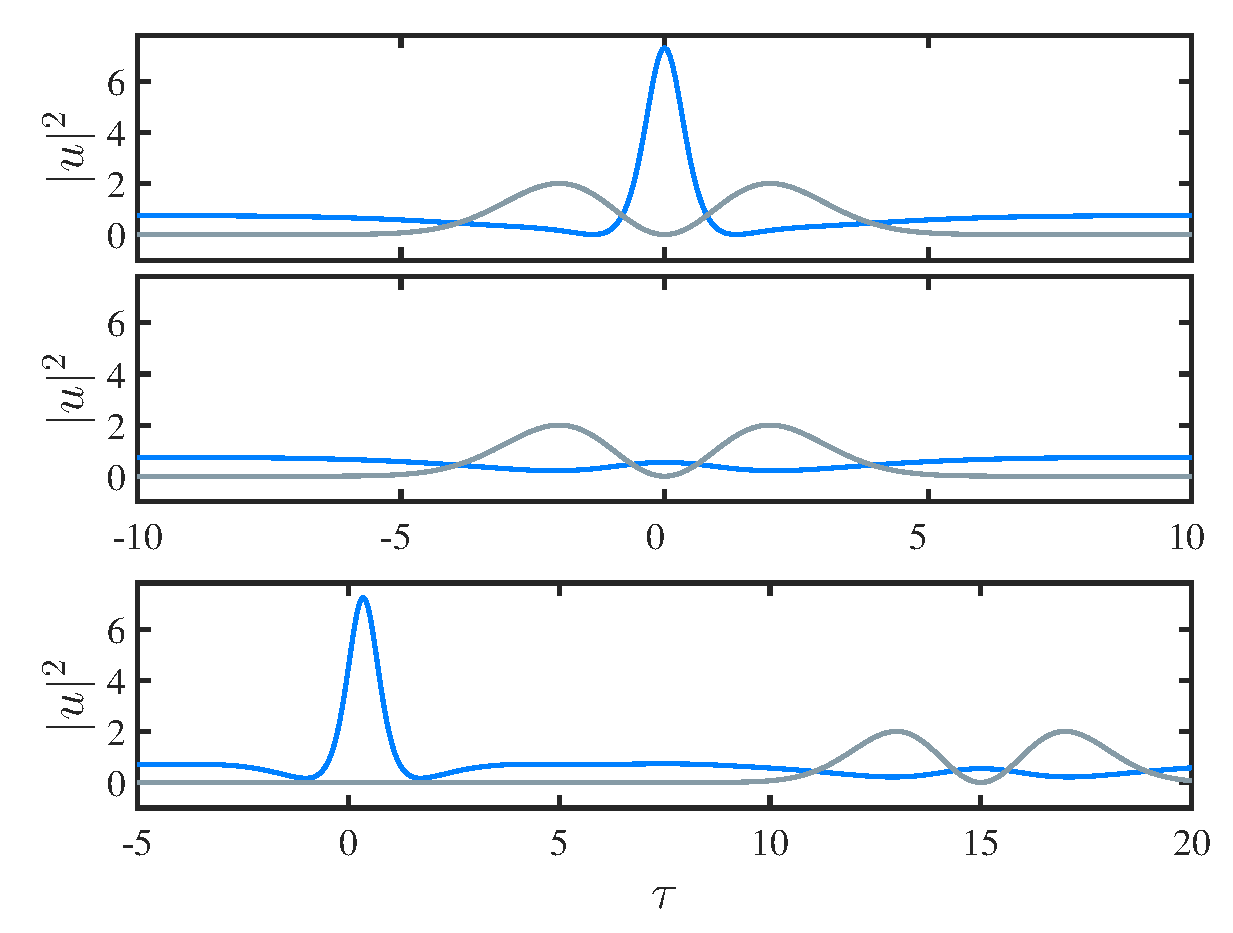
\includegraphics[width=0.9\textwidth]{threeStates.eps}}
  \rule{35em}{0.5pt}
\caption[Temporal Profiles of Fundamental States]{Temporal profiles of the intracavity field envelope $|u|^2$ (blue line) for the most fundamental nonlinear states of the system.  In this example, the effective potential, $V_{\mathrm{eff}} = (\phi')^2$ (solid grey line) is constant in the three panels.  The top panel is an example of a trapped CS (tweezed CS).  The middle panel is an example of no soliton solution (no-CS).  The bottom panel has an effective potential centered at $\tau_0 = 15$.  The CS is located outside of the effective potential, and a no-CS is found inside the effective potential (called non-tweezed CS).  
}
\label{fig:threeStates}
\end{figure}

We now proceed to provide a characterization of the existence of the three states for the full LL Eq.~(\ref{eq:LLETweeze}) and compare to the results of the NCVA with respect to the parameters $\beta$ and $\tau_f$.  In what follows, we study different tweezing possibilities over the parameter space spanned by $\tau_f$, the final temporal displacement, and $\beta$, the degree of adiabaticity for the speed of the tweezer.  A fully tweezed CS will correspond to a CS that stays inside the effective potential as the tweezer is displaced.  

Rather than analyzing the individual evolution of temporal profiles, we can express the various states by the power contained inside and outside of the effective potential.  For the full LL model, the CS temporal density $\rho = |u|^2$ and the no-CS temporal density $\rho_0 = |u_{\rm{no\text{-}CS}}|^2$ are expressed by the power inside the tweezer $P_{\rm I}(z)$ and outside the tweezer $P_{\rm O}(z)$ which are given respectively by 
\begin{align}
P_{\rm I}(z) = \int_{\rm D} (\rho - \rho_0) d\tau, \label{Pin} \\
P_{\rm O}(z) = \int_{\bar{\rm D}} (\rho - \rho_0) d\tau, \label{Pout}
\end{align} 
where \JMR{${\rm D} = [ -\sigma_{\phi}, \sigma_{\phi}]$} is the domain of the tweezer which is defined as a small symmetric interval around $\tau_0$ between the maxima of the effective trap and its complement, $\bar{\rm{D}}$.  We need to subtract the no-CS power, $\rho_0$ in order to counter the effects of the pedestal (constant steady state) and insure the power for a CS is positive.  The total power of the system is given by 
\begin{align}
P_{\rm Tot} = \int  (\rho - \rho_0) d\tau.
\end{align}
Recall that in the construction of the NVCA ansatz we already subtracted out the effects of the background pedestal.  For the NCVA, we use the variational parameters and construct the CS temporal density $\bar{\rho} = |\bar{u}|^2$ and extract the power inside the tweezer $P_{\rm I}(z)$ and outside the tweezer $P_{\rm O}(z)$ which are given, respectively, by 
\begin{align}
P_{\rm I}(z) = \int_{\rm D} \bar{\rho }d\tau, \label{PinNCVA} \\
P_{\rm O}(z) = \int_{\bar{\rm D}} \bar{\rho } d\tau, \label{PoutNCVA}
\end{align} 
where ${\rm D}$ and $\bar{{\rm D}}$ are the same intervals described above.
%Due to the construction of the NCVA ansatz, $\rho_0 = 0$ since the background pedestal is removed and the no-CS solution of the NCVA tends toward zero (not $v$ as described by the full LL model). 
The power ratio parameters inside, $Q_{\rm I}$, and outside, $Q_{\rm O}$, the tweezer are then defined, respectively, by 
\begin{align}
Q_{\rm I} = \frac{P_{\rm I}(0) - P_{\rm I}(z_f)}{P_{\rm Tot} },\label{QIn} \\ 
Q_{\rm O}=  \frac{P_{\rm O}(0) - P_{\rm O}(z_f)}{P_{\rm Tot} }.
\label{QOut}
\end{align}
By considering $Q_{\rm I}$ and $Q_{\rm O}$, we can effectively find the thresholds between the various states in the relevant ($\beta$, $\tau_f$) parameter space.  

\begin{figure}[p!]
\centering
\center{
\centerline{
\begin{subfigure}{\textwidth}
\hspace{0.5cm}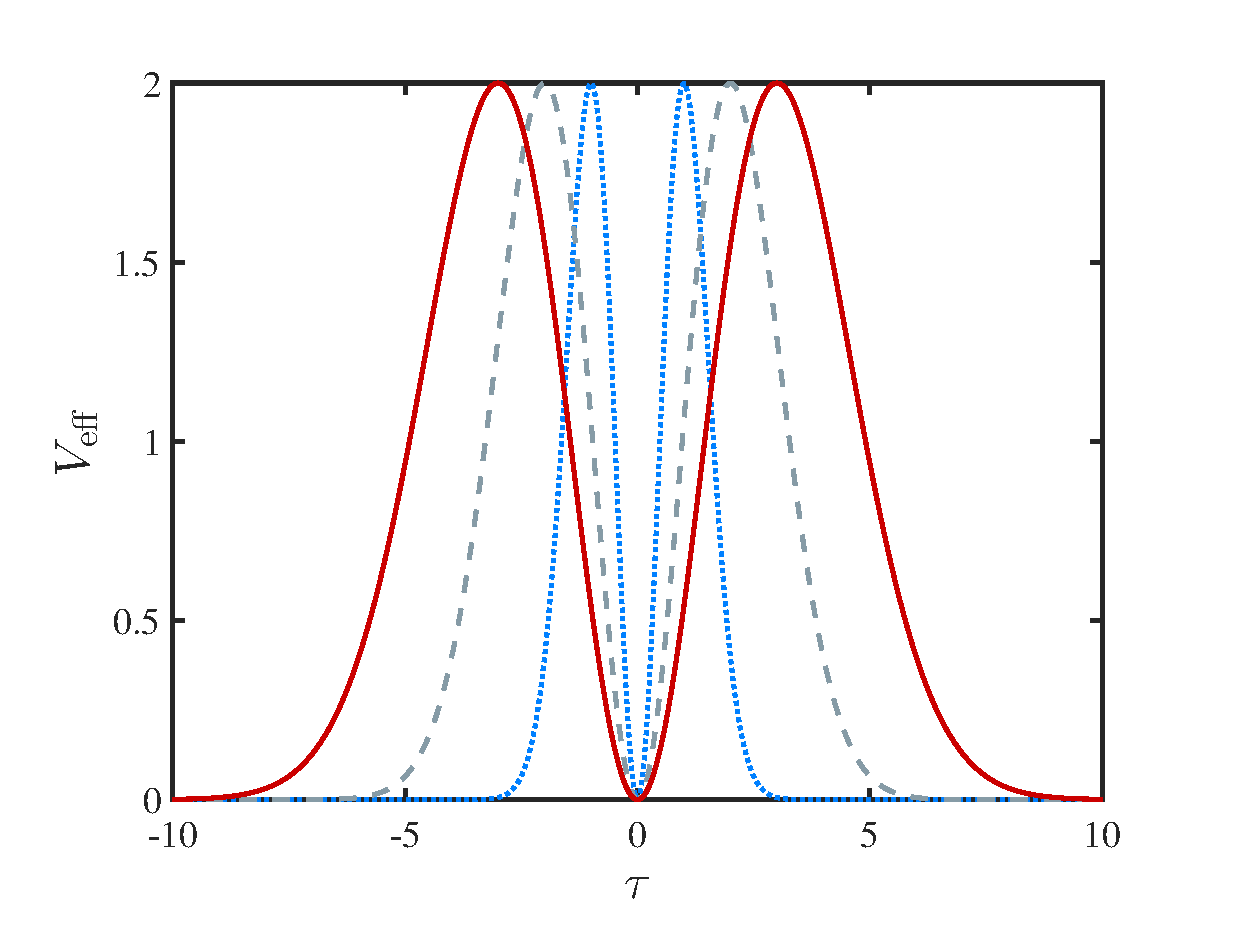
\includegraphics[width=0.9\linewidth]{potentials.eps}
\caption{}
\end{subfigure}}
\centerline{
\begin{subfigure}{\textwidth}
\hspace{0.5cm}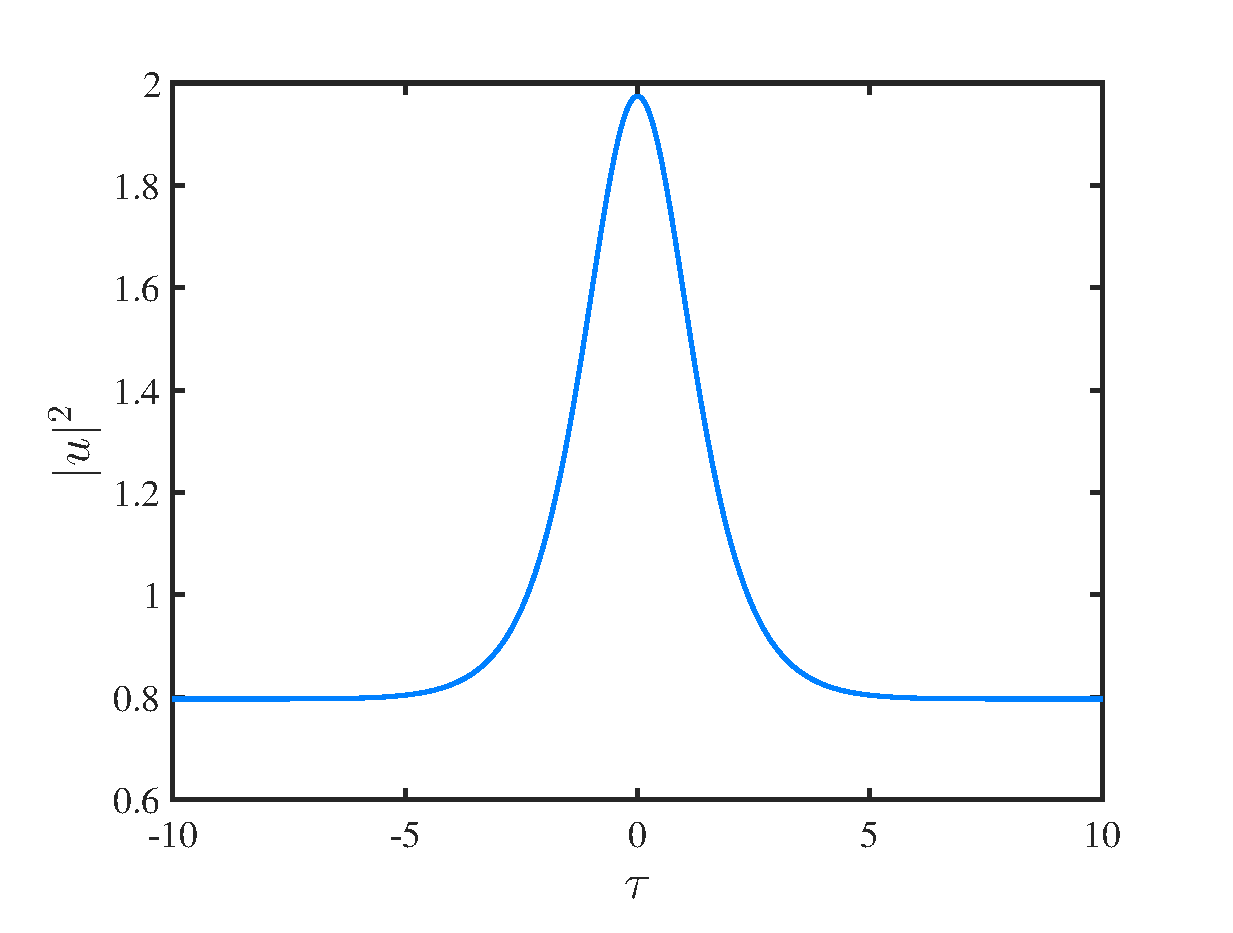
\includegraphics[width=0.9\linewidth]{noTrapCS.eps}
\caption{}
\end{subfigure}}}
  \rule{35em}{0.5pt}
\caption[Tweezers of Narrow, Natural, and Wide Widths]{(a) Tweezers consisting of effective potentials of constant height with narrow, natural and wide widths.  The narrow width tweezer (blue dotted line) is composed of phase modulation with $\sigma_\phi = 1$ and $h_\phi = 2.3316$ solved with Eq.~(\ref{height}).  The natural width tweezer (grey dashed line) is composed of phase modulation with $\sigma_\phi = 2$ and $h_\phi = 4.6633$ solved with Eq.~(\ref{height}).  The wide width tweezer (red solid line) is composed of phase modulation with $\sigma_\phi = 3$ and $h_\phi = 6.9949$ solved with Eq.~(\ref{height}). (b) The density of a cavity soliton in the absence of a tweezer, which has a natural width of ~1.5.  
}
\label{fig:Veff}
\end{figure}


For example, if we begin with a steady state CS inside the tweezer at $\tau_0=0$ and move with a given $\beta$ and $\tau_f$, then a perfectly tweezed CS will result on the same powers at $z=0$ as $z = z_f$ such that $P_{\rm I}(0) =  P_{\rm I}(z_f)$ as well as $P_{\rm O}(0) = P_{\rm O}(z_f)$, making the power ratios $Q_{\rm I} = Q_{\rm O} = 0$.   If the CS dissipates perfectly and we are left solely with no-CS inside the tweezer, then $Q_{\rm I} = 1$ and  $Q_{\rm O} = 0$.  For the final non-tweezed CS state, at $z=z_f$ the CS is completely outside the tweezer, and a no-CS is inside the tweezer, at which point $Q_{\rm I} = Q_{\rm O} = 1$ .   

For our analysis, we select three tweezers with a fixed height and a narrow, natural, and wide width corresponding to $\sigma_\phi = 1$, 2, and 3, respectively.  In order to maintain a constant maximum height of the effective potential $V_{\rm eff}$ equal to 2 (such that we have a deep enough trap to contain the CS and is the height of a natural CS in the absence of a tweezer [see Fig.~\ref{fig:Veff}(b)]), we solve for the height of Eq.~(\ref{phi}) 
\begin{align}
h_\phi = \frac{\sqrt{2} \sigma_{\phi}^2}{\max [\tau \exp(-\tau^2/2\sigma_{\phi}^2)]}.
\label{height}
\end{align}
Figure~\ref{fig:Veff}(a) depicts the effective potentials $V_{\rm eff} = (\phi')^2$ used in the three tweezer cases we are interested in studying: tweezers with (i) narrow width $\sigma_\phi = 1$ (blue dotted line) in Sec.~\ref{section:Skinny}, (ii) natural width $\sigma_\phi = 2$ (grey dashed line) in Sec.~\ref{section:Regular}, and (iii) wide width $\sigma_\phi = 3$ (red solid line) in Sec.~\ref{section:Fat}.  For comparison, Fig.~\ref{fig:Veff}(b) shows the density of a CS in the absence of a tweezer, which has a natural width $\sigma \approx 1.5$.  For all example cases to follow, we keep the holding beam constant at $u_{\rm in} = 2$.

\setstretch{1.3}
\subsection[Tweezer with Narrow Width]{Tweezer with Narrow Width} \label{section:Skinny}
\setstretch{2}

In the first case study, we are interested in a tweezer with a narrow width $\sigma_\phi = 1$ and height $h_\phi = 2.3316$ given by Eq.~(\ref{height}).  For the full LL Eq.~(\ref{eq:LLETweeze}), the steady state CS is found centered at $\tau_0 = 0$ using a Newton-Krylov solver and the power-balance constraint Eq.~(\ref{LLConstraint}) which selects a detuning parameter value of $\Delta =  4.1692$.  The same $\Delta$, $\sigma_\phi$, and $h_\phi$ are used in the NCVA with a Newton-Krylov solver to find the initial variational parameters for the system.  The parameter space for $\beta$ and $\tau_f$ are discretized into 41 steps between 0.1 and 20, giving 1681 combinations for $\tau_0(z)$ [Eq.~(\ref{tau0})].  \JMR{For this example, the parameter space is excessive for the narrow width tweezer.  In the next two examples for natural and wide width tweezer we will need the entire parameter space to characterize the dynamics of tweezing.}  The full LL Eq.~(\ref{eq:LLETweeze}) is solved using a Runge-Kutta method in time and finite differences in space \JMR{with periodic boundary conditions for the ring cavity} and the NCVA system of ODEs are solved using Matlab's ode15s.  It is important to note, the NCVA requires a stiff ODE solver to produce the numeric results. 
%Also, at this time we should mention the time-varying ode15s has a speedup of XX compared to fixed time ode15s.  There is also a XX speedup between the PDE Runge-Kutta solver and the ODE solver ode15s.  
Both the full LL equation and NCVA evolve until $z_f = 10 = 4z^*$, with $z^* = 2.5$ which ensures that the tweezed and/or non-tweezed CS have enough time to converge towards their steady state. 

\begin{figure}[p]
\centering 
\centerline{
\hspace*{0cm}
\begin{subfigure}{0.5\textwidth}
\hspace{0.6cm}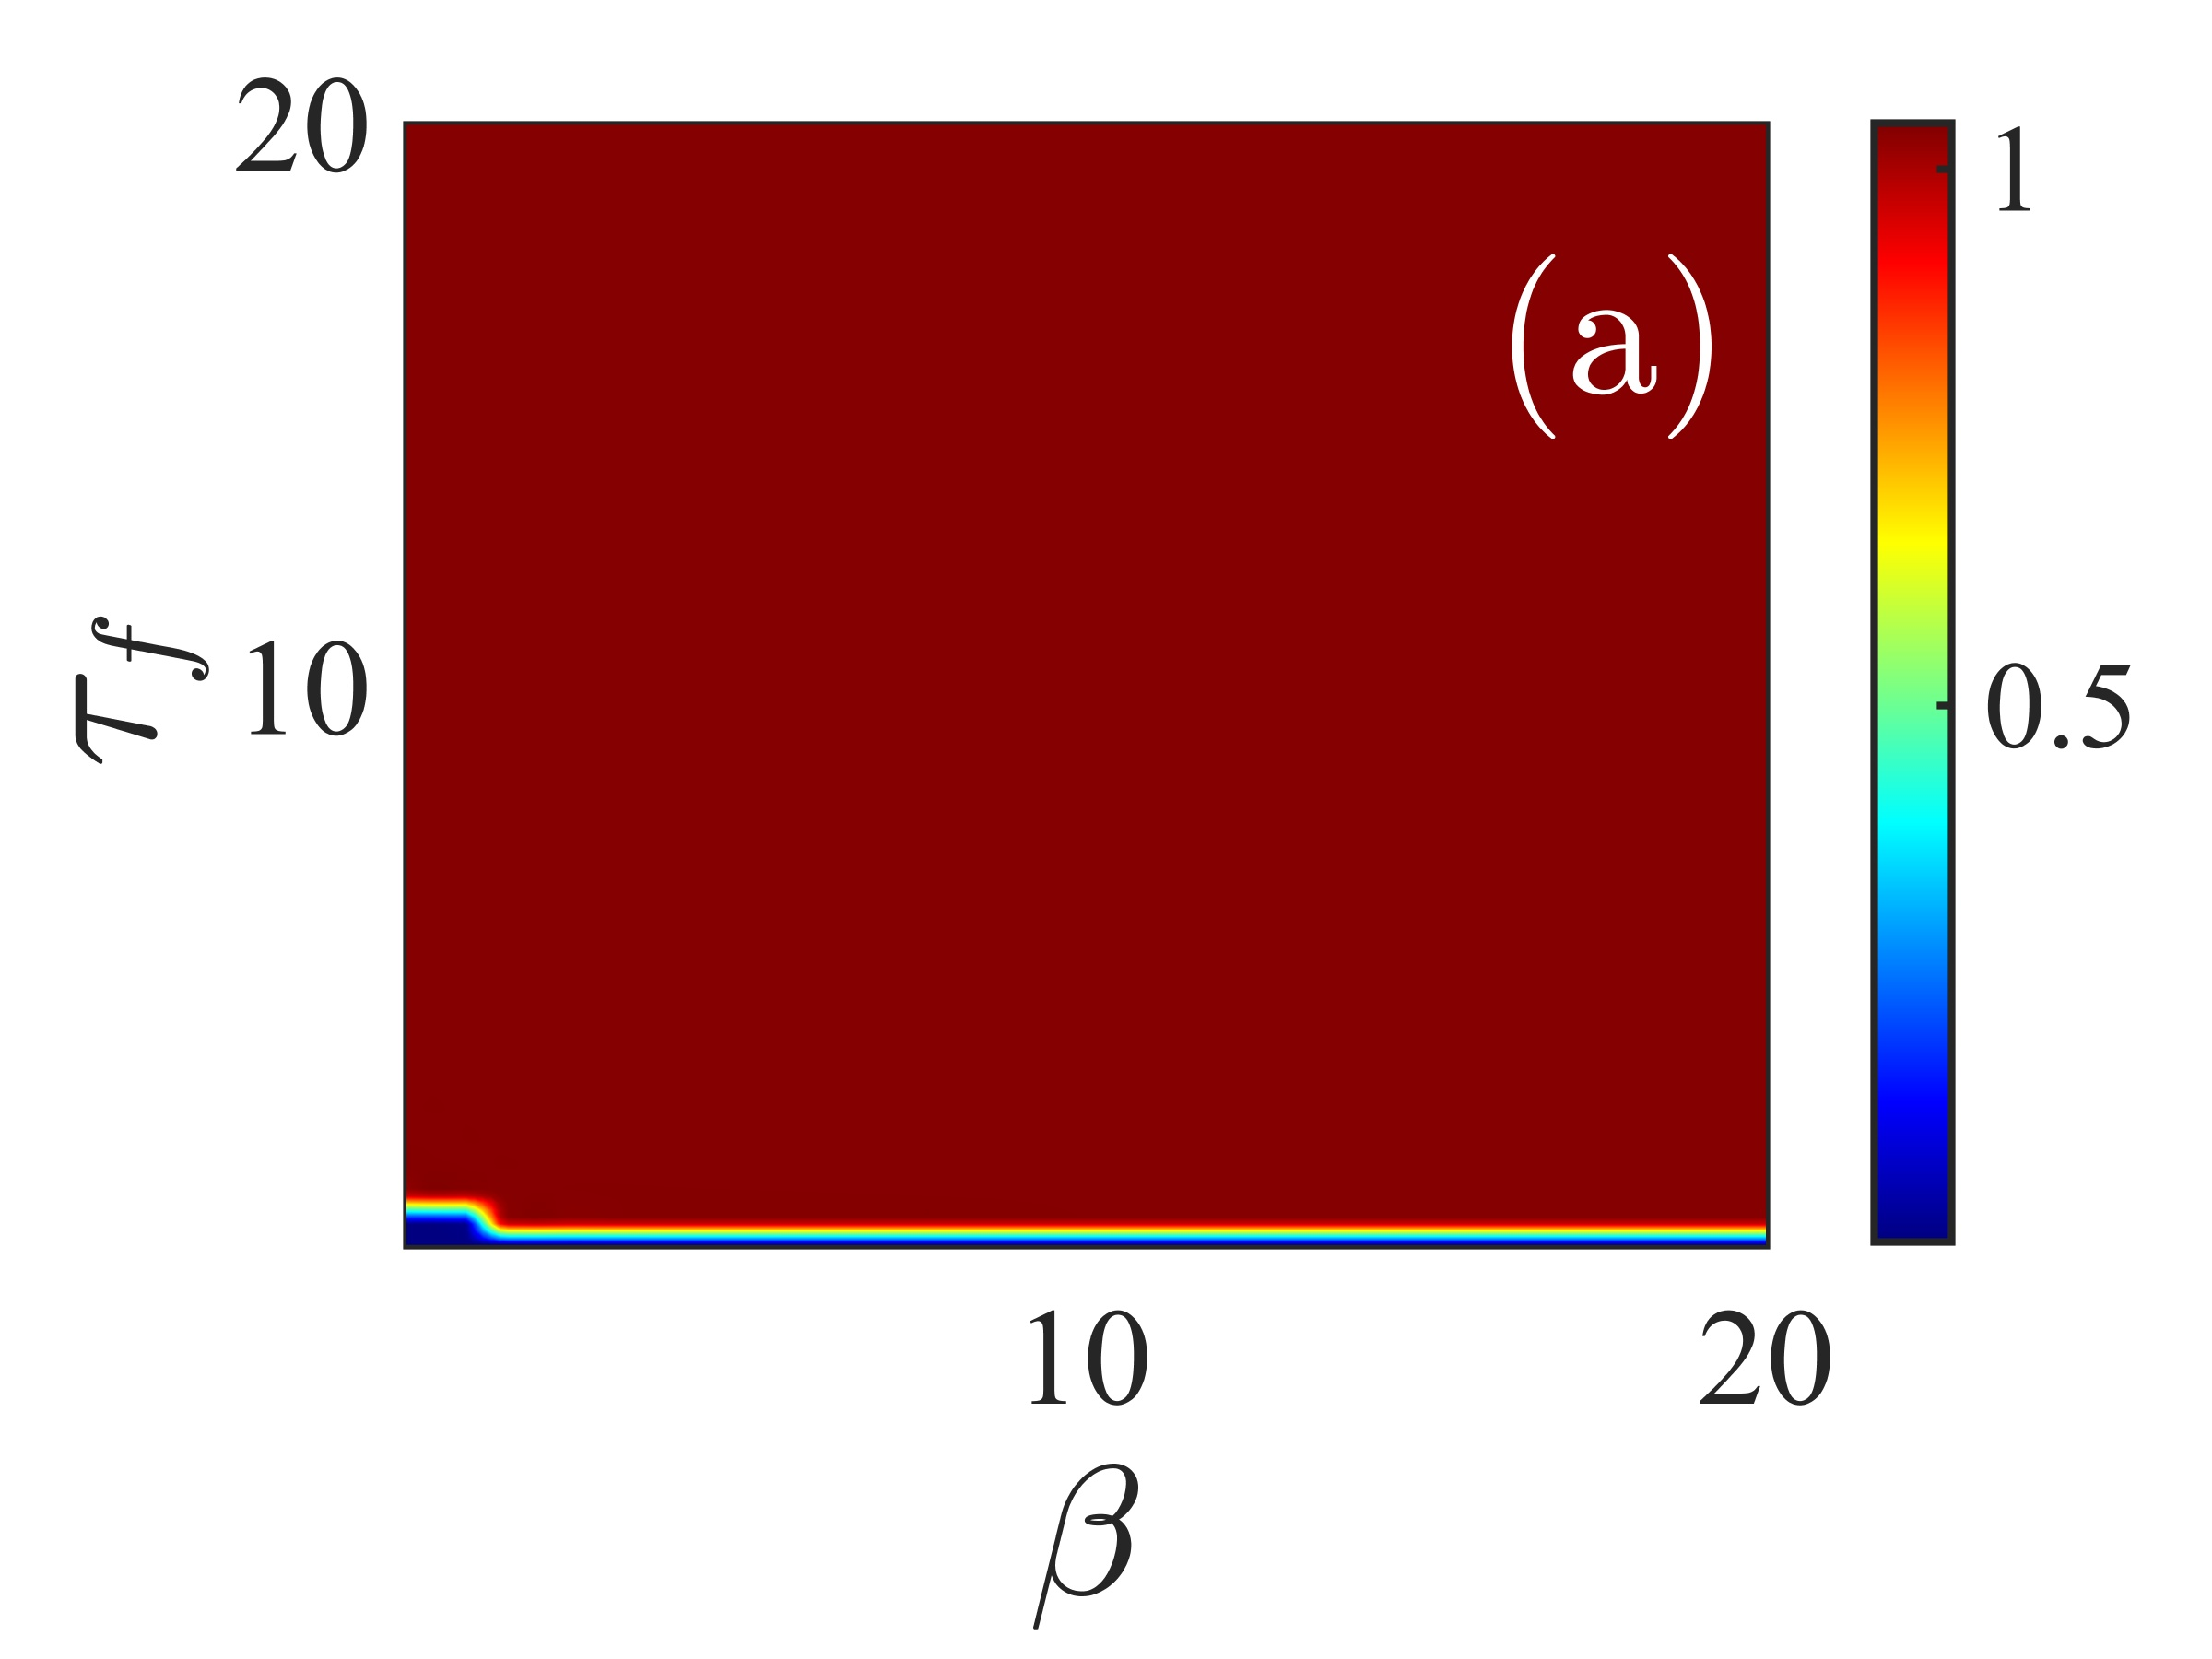
\includegraphics[width=\linewidth]{SkinnyQIn.jpg}
\caption{} 
\end{subfigure}
%\hspace*{\fill}
\begin{subfigure}{0.5\textwidth}
\hspace*{0cm}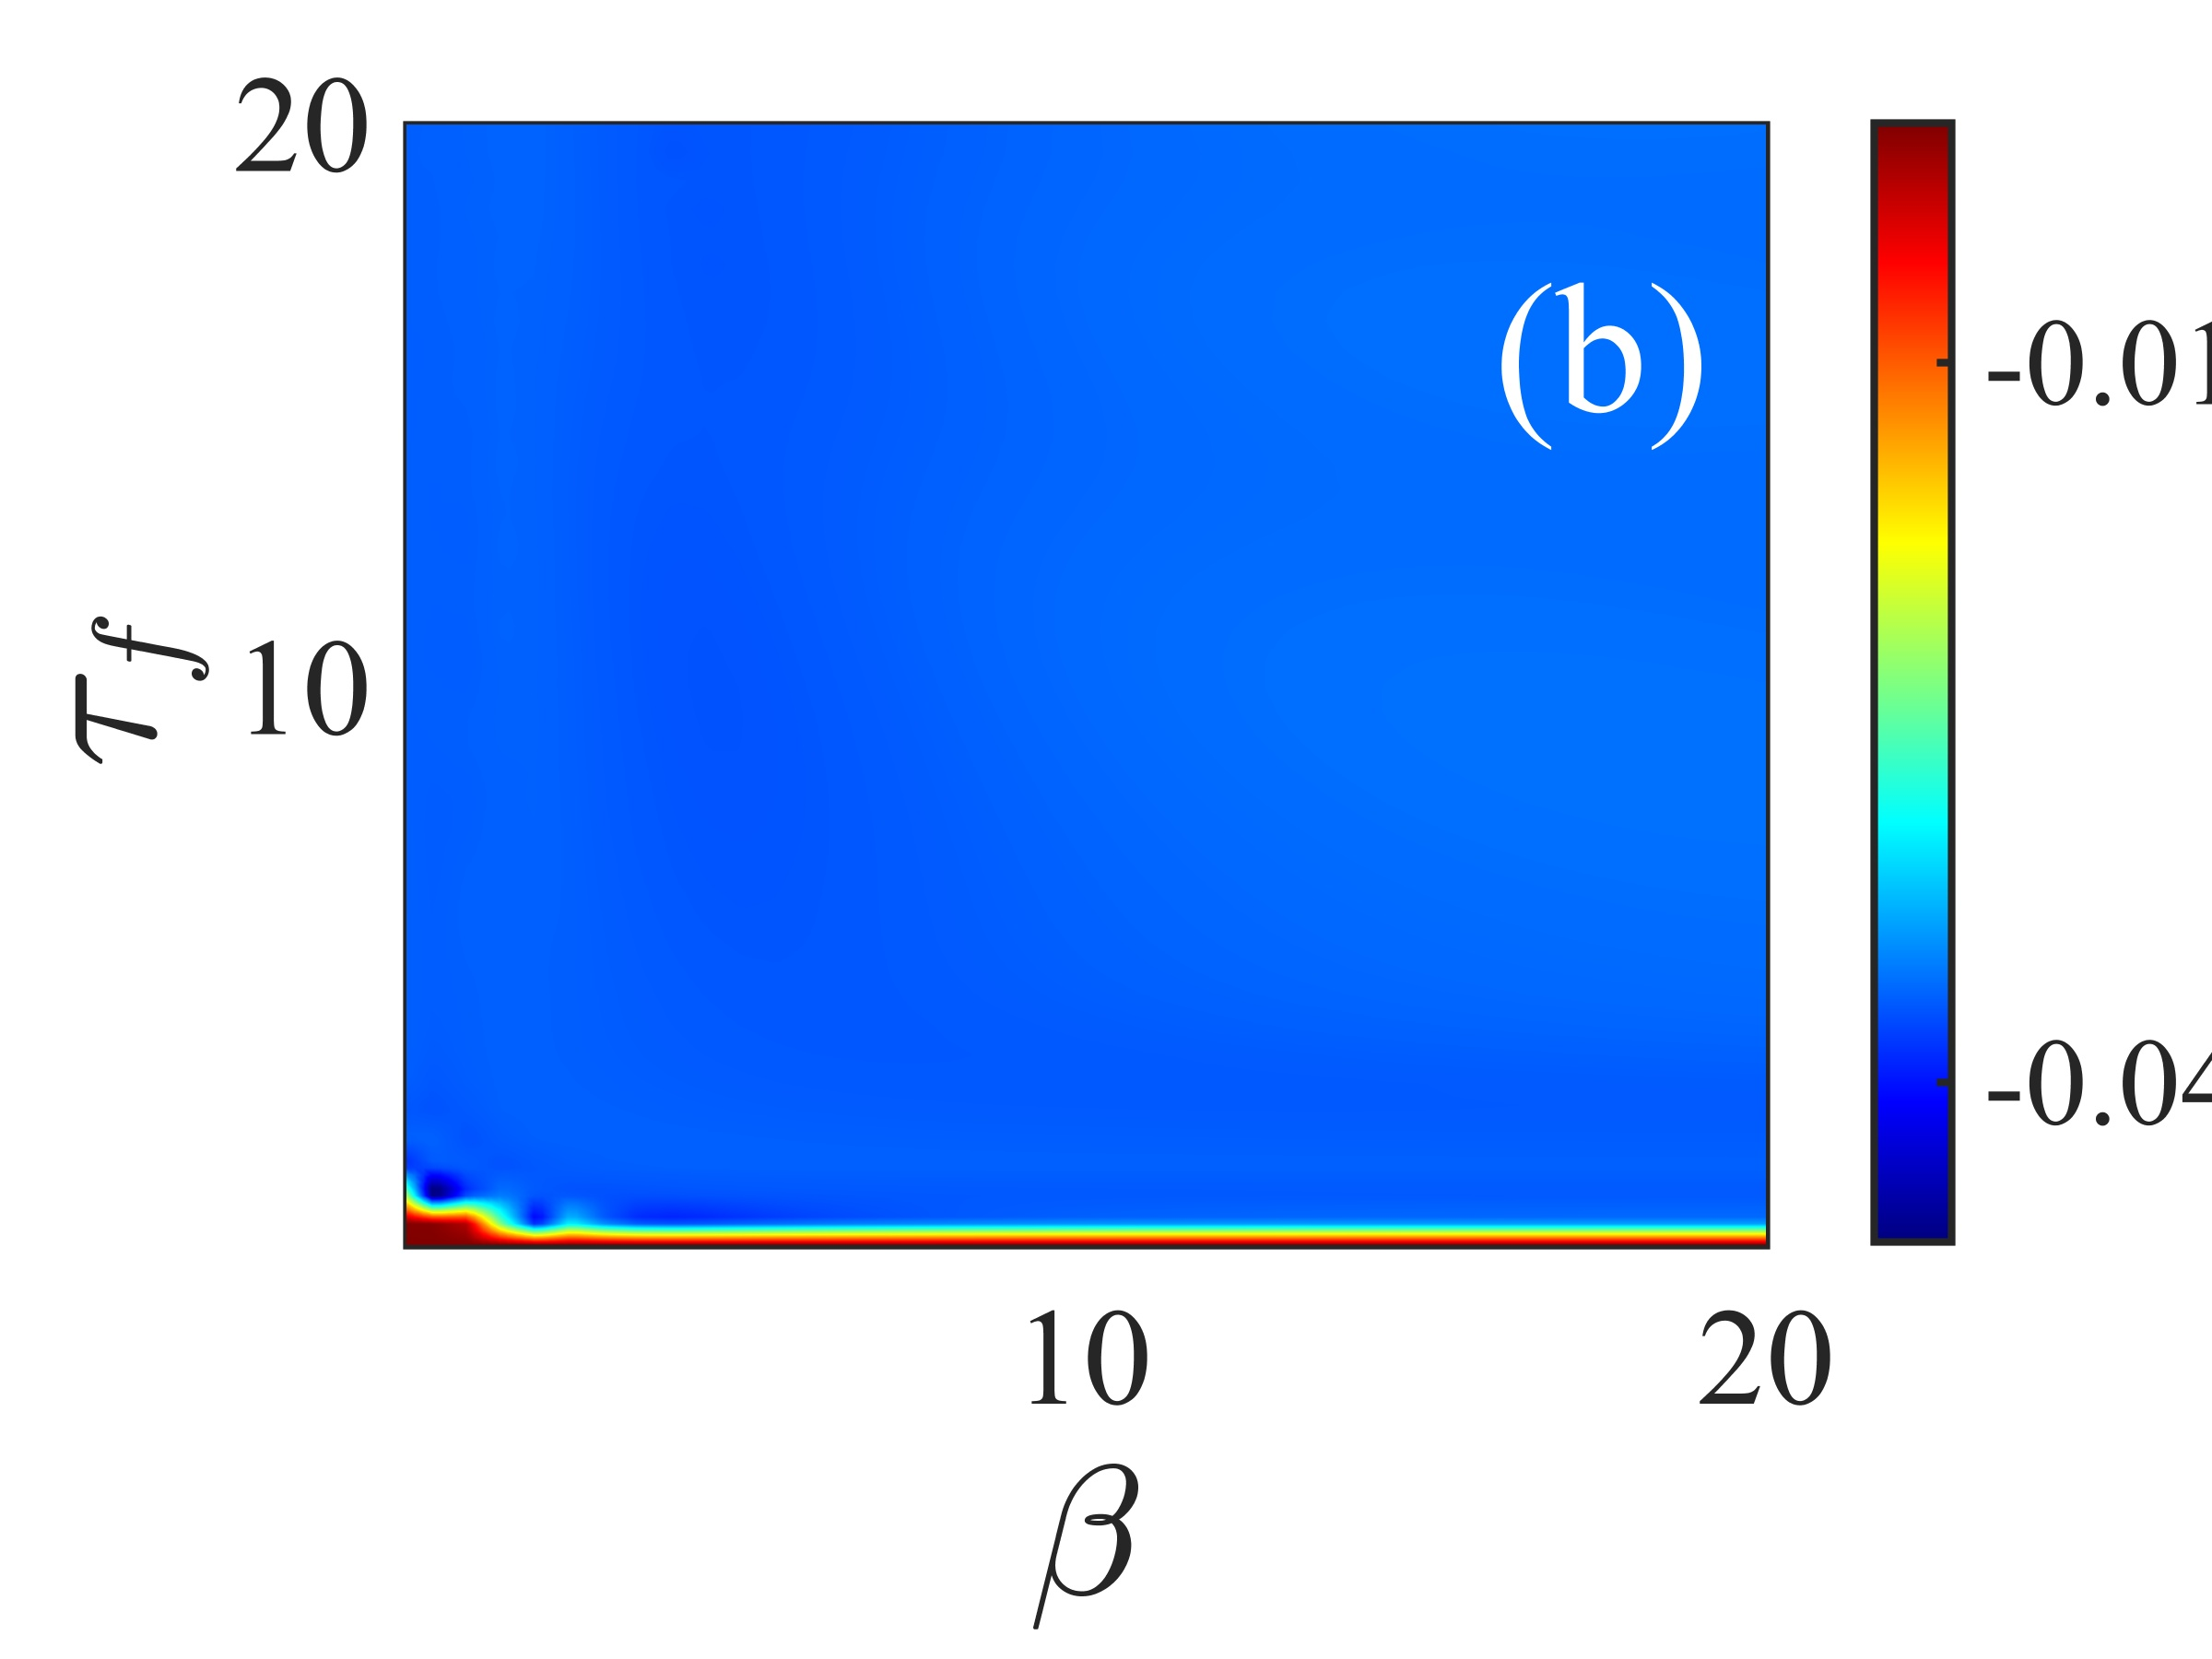
\includegraphics[width=\linewidth]{SkinnyQOut.jpg} 
\caption{} 
\end{subfigure} }
\centering
\centerline{
\begin{subfigure}{\textwidth}
\hspace{0.6cm}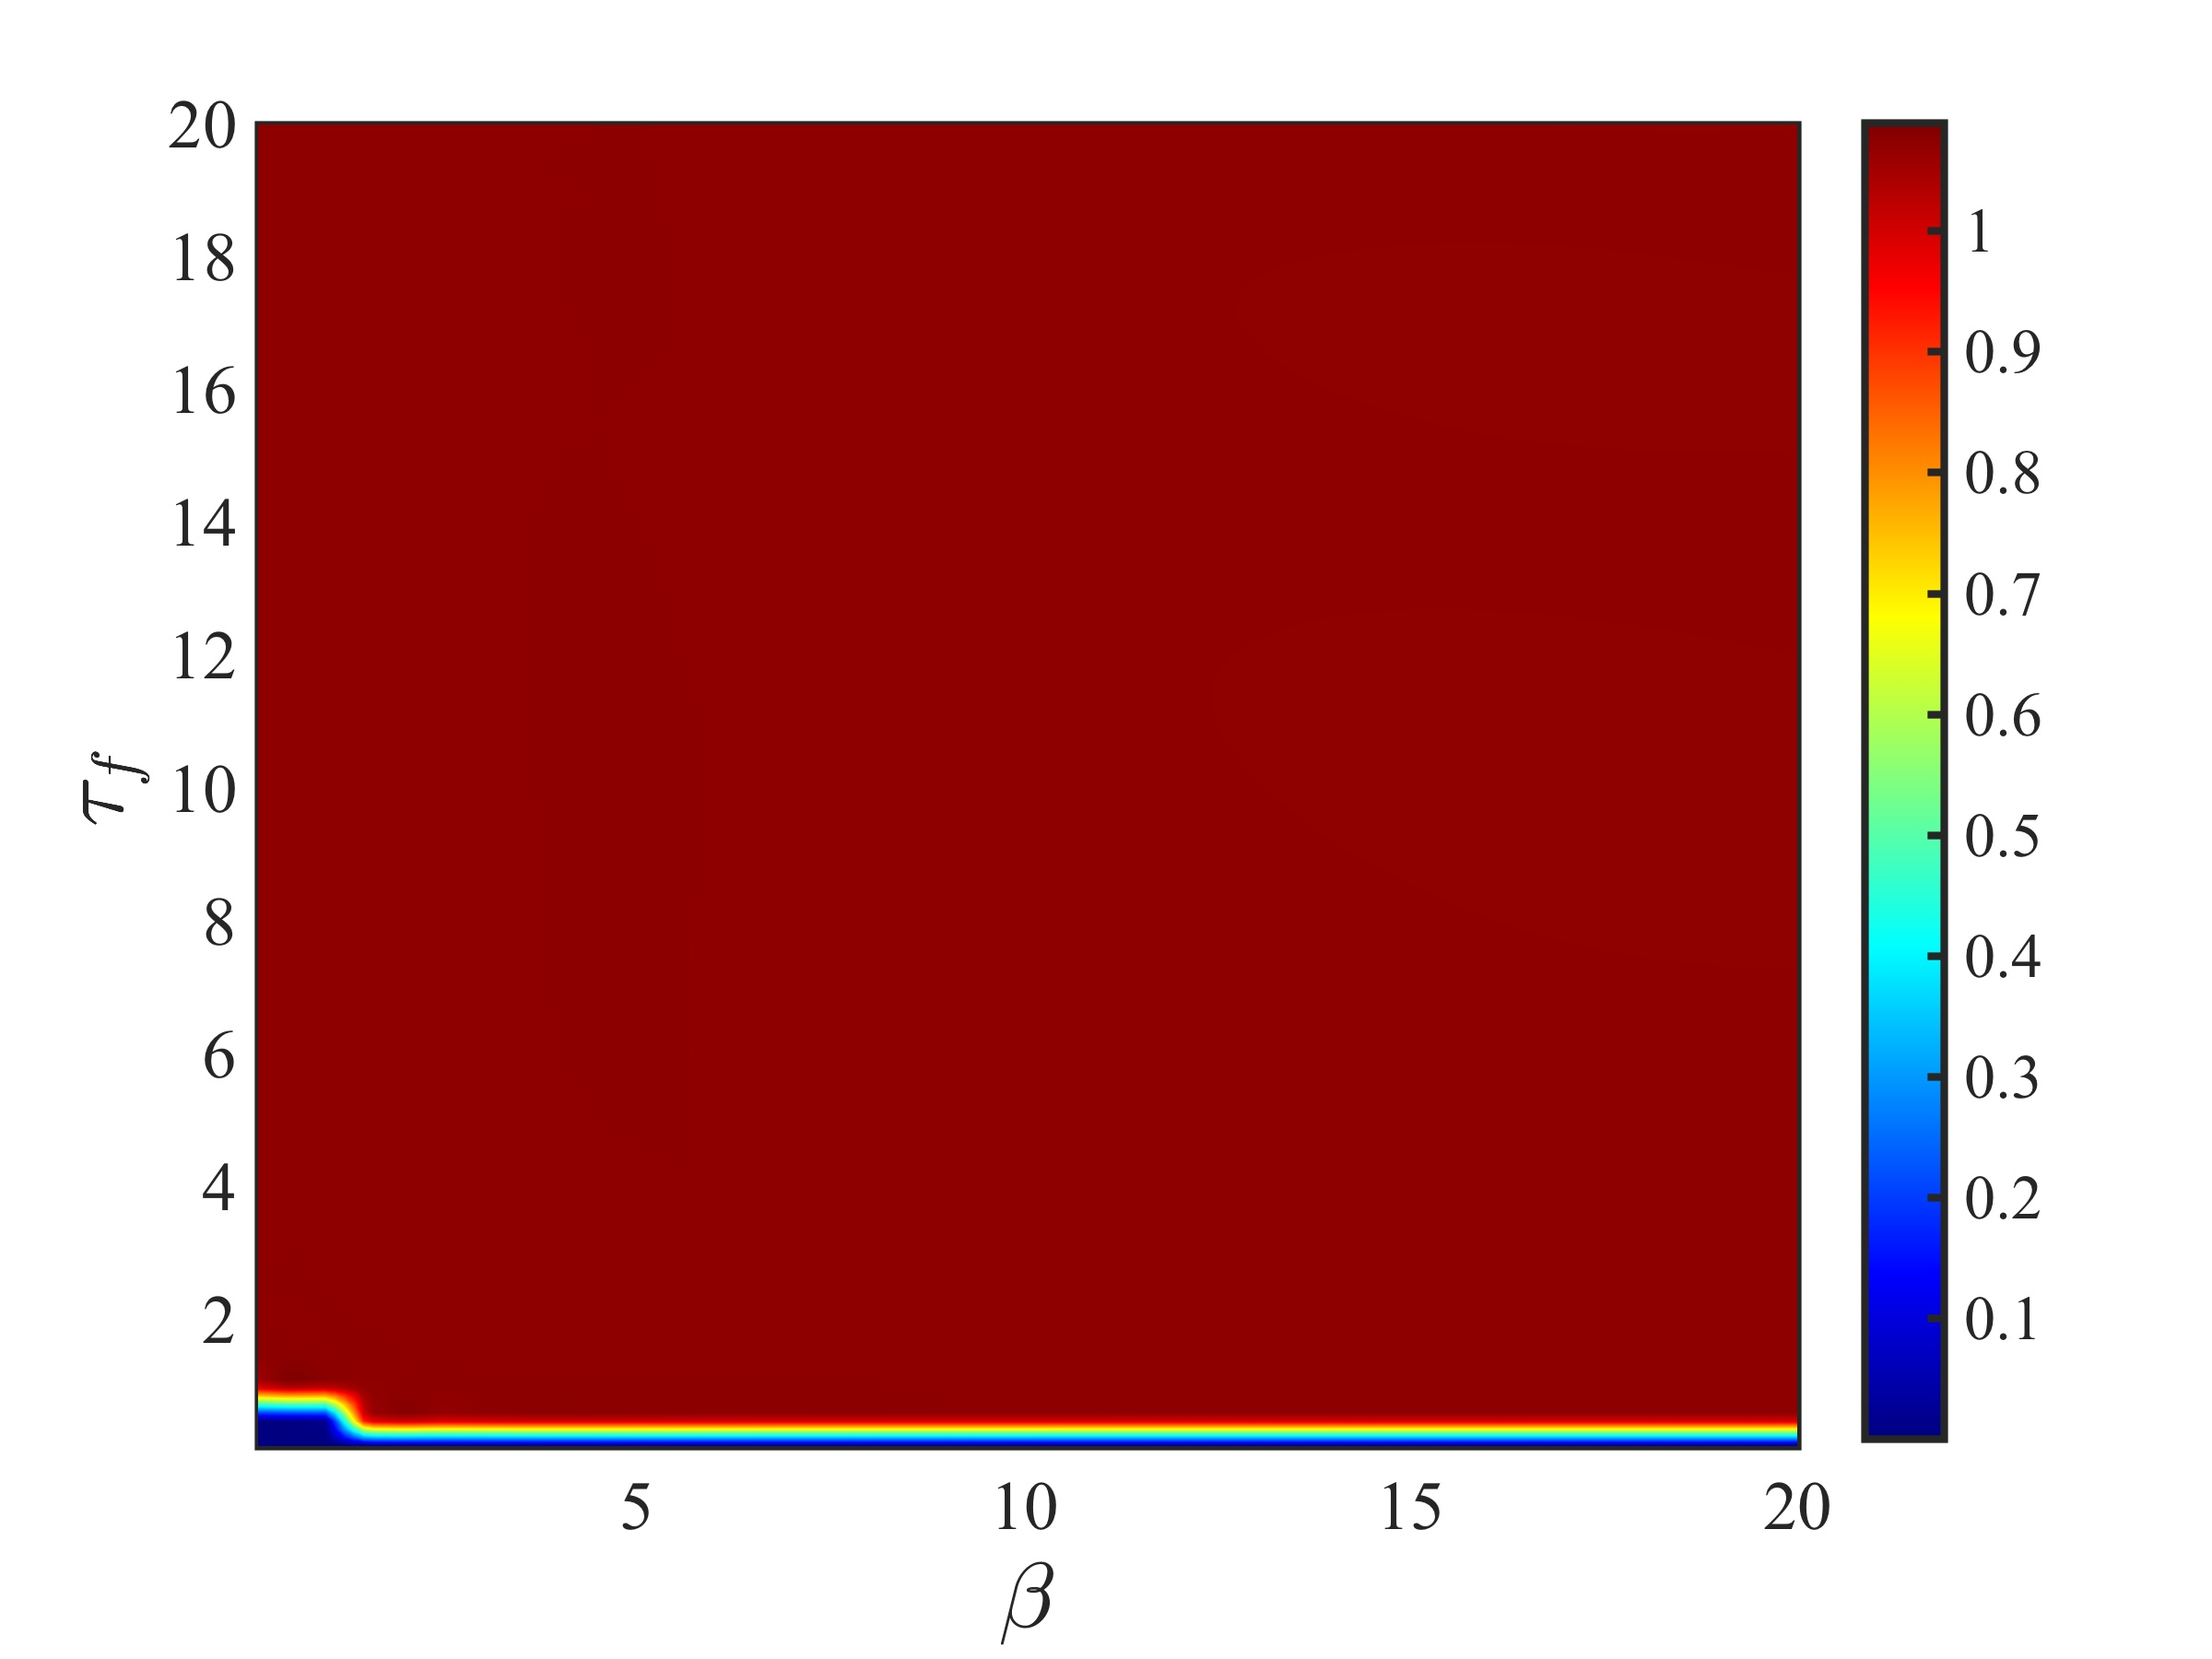
\includegraphics[width=\linewidth]{SkinnyQDiff.jpg} 
\caption{} 
\end{subfigure} }
  \rule{35em}{0.5pt}
\caption[Power Ratios Inside and Outside Tweezer with Narrow Width]{The density of the power ratios (a) inside and (b) outside of a narrow tweezer width $\sigma_\phi = 1$ and height $h_\phi = 2.3316$.  The detuning for the system is $\Delta =  4.1692$ and each combination of parameter is evolved for $z_f = 10 = 4z^*$, with $z^* = 2.5$.  \JMR{The parameter space of $\beta$ and $\tau_f$ was chosen to capture the three fundamental nonlinear states in the case of the natural width tweezer and is excessive for this example.}  (a) The power ratio density inside the tweezer $Q_{\rm I}$, where blue ($Q_{\rm I}=0$) is complete power inside the tweezer at $z_f$ and red ($Q_{\rm I}=1$) is no power inside the tweezer at $z_f$.  (b) The power ratio density outside the tweezer $Q_{\rm O}$, where $Q_{\rm O}$ = 0 depicts no change in power.  (c) The difference in power ratios inside and outside the tweezer, $Q_{\rm I} - Q_{\rm O}$.   For the difference of power ratios, a value of 1 is a non-tweezed CS, a value of 0.5 is a no-CS, and a value of 0 is a tweezed-CS.  The difference power ratio defines the threshold between two fundamental states: a tweezed CS for all $\beta$ when $\tau_f \le 0.1$ and no-CS for all other parameter space.  
}
\label{fig:SkinnyQ}
\end{figure}


\begin{figure}[htb!]
\centering
\centerline{
\begin{subfigure}{0.5\textwidth}
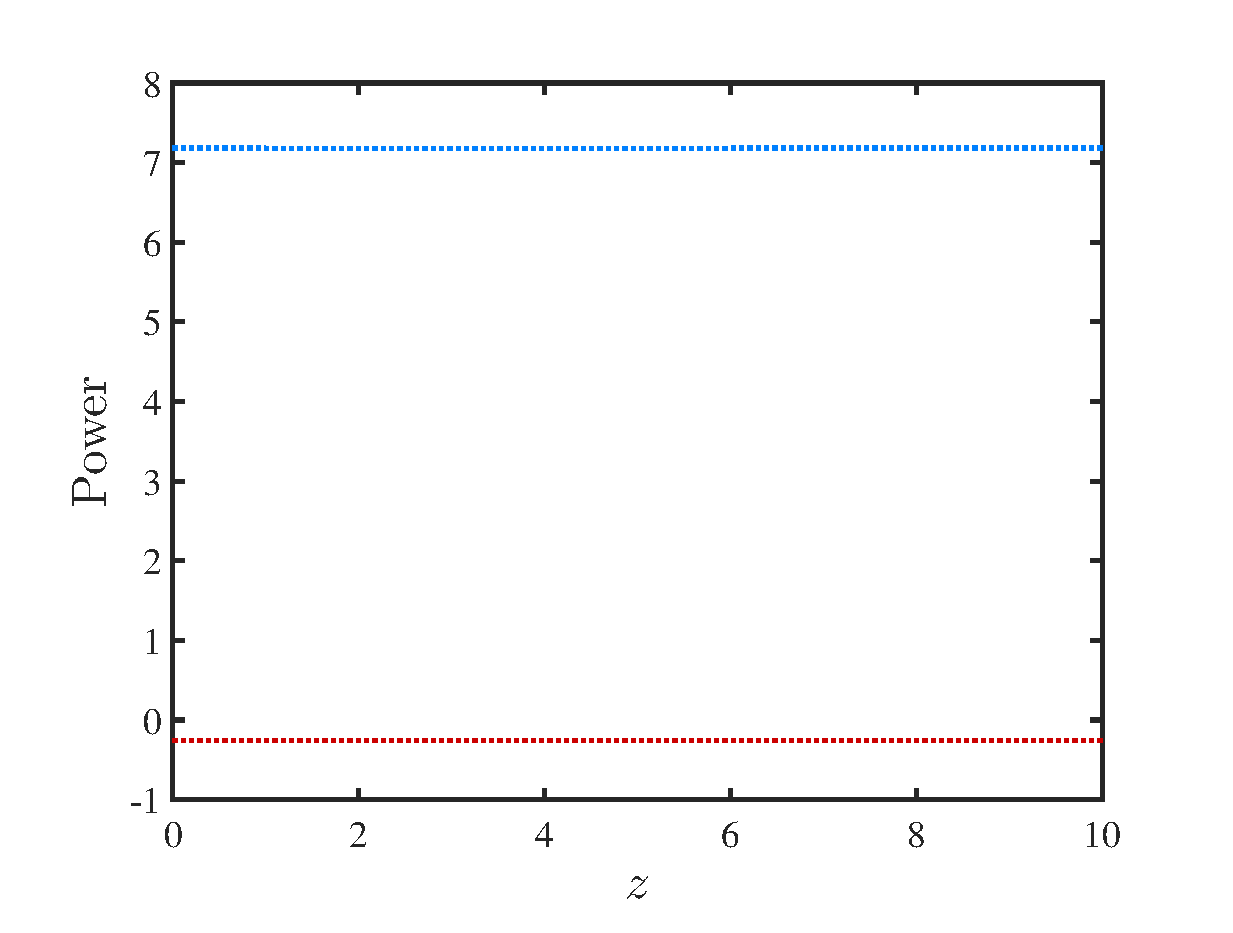
\includegraphics[width=\linewidth]{skinnyTimeMass1.eps} 
\caption{}
\end{subfigure}
\begin{subfigure}{0.5\textwidth}
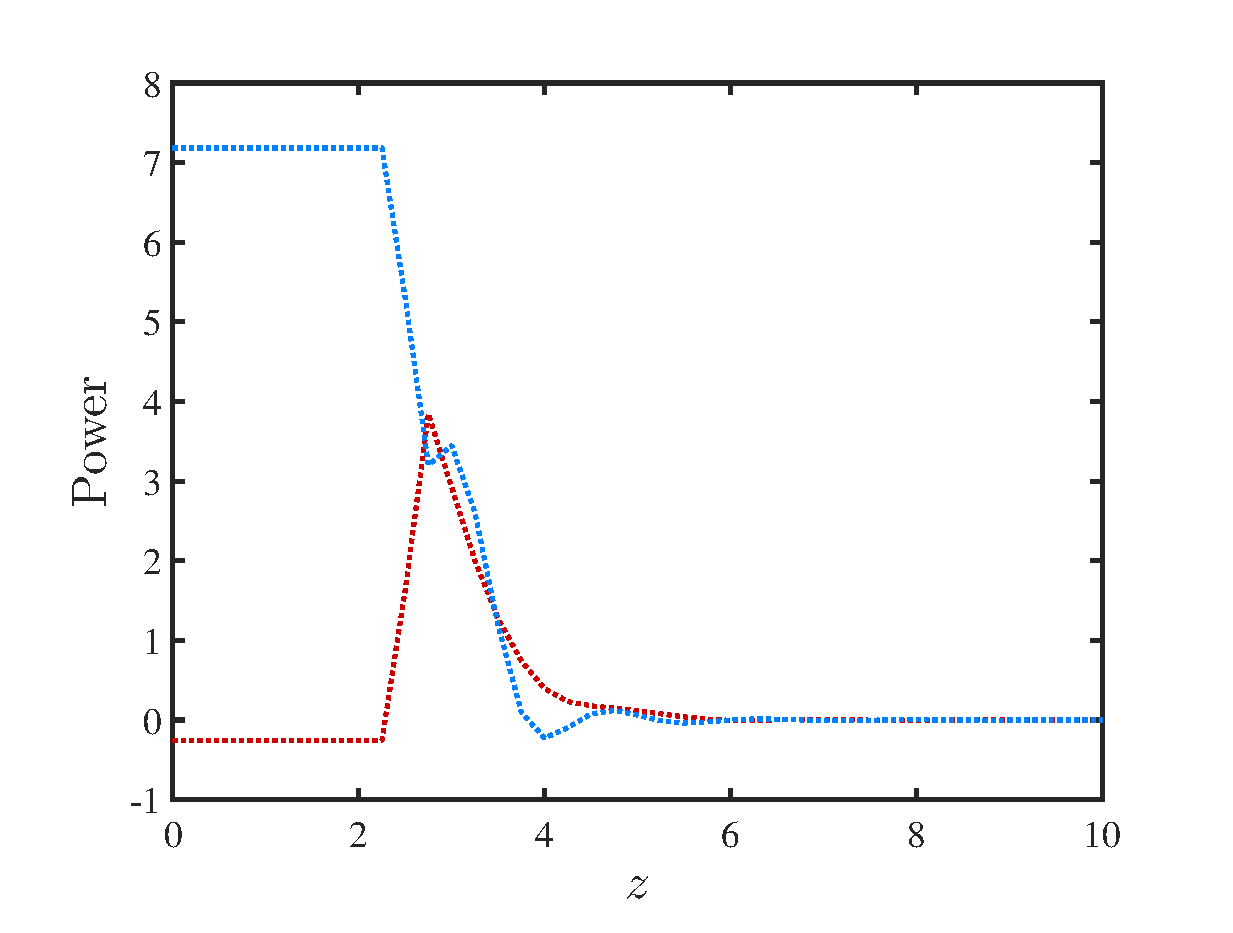
\includegraphics[width=\linewidth]{skinnyTimeMass3.eps} 
\caption{}
\end{subfigure} 
}
\rule{35em}{0.5pt}
\caption[Tweezer with Narrow Width Power Comparison]{Comparison of the powers found inside the tweezer $P_{\rm I}$ (red line) and outside the tweezer $P_{\rm O}$ (blue line) for the parameters (a) $\tau_f = 0.1$ and $\beta=0.1$, with no change in power inside or outside the tweezer which describes a tweezed CS and (b) $\tau_f = 2$ and $\beta = 10$, with no change in power outside the tweezer and complete loss of power inside the tweezer describes a dissipative no-CS solution.  
}
\label{fig:SkinnyComp}
\end{figure}

\begin{figure}[htb!]
\centering
\centerline{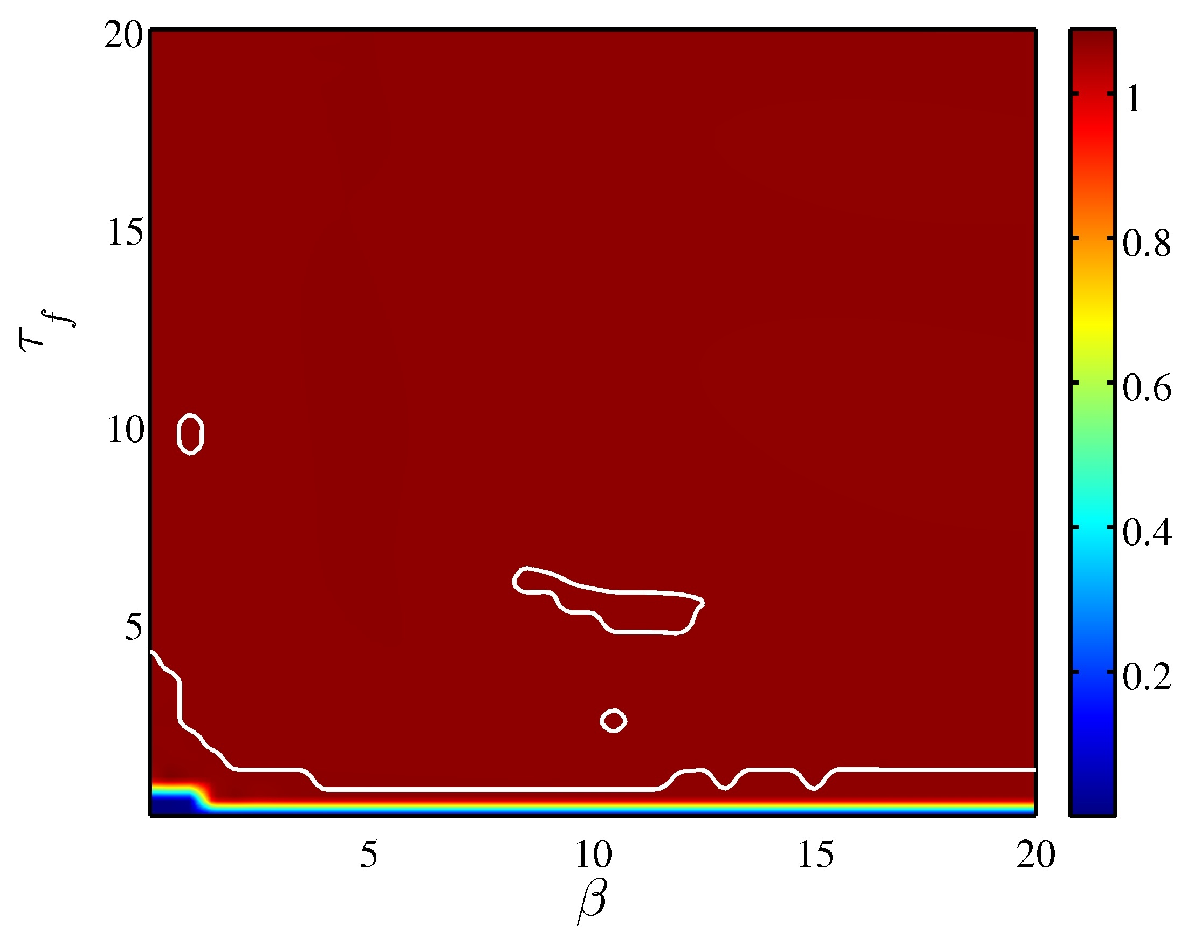
\includegraphics[width=0.9\textwidth]{SkinnyPDEvODE_rcg_t.eps}}
  \rule{35em}{0.5pt}
\caption[Comparison of Power Ratio Inside Narrow Tweezer for LL Model and NCVA]{The density of the difference of power ratios inside of a narrow tweezer in the parameter space of $\tau_0$ for the full LL model (same as Fig.~{fig:SkinnyQ}(c)) with a single contour at 0.5 (white line) for the NCVA threshold between tweezed and non-tweezed states.  For the difference of power ratios, a value of 1 is a non-tweezed CS, a value of 0.5 is a no-CS, and a value of 0 is a tweezed-CS.  The white contour line distinguishes the NCVA region between a solutions with tweezed CS and dissipative solutions with no-CS.  For the narrow width tweezer, the full LL model has a very small region of tweezed-CS for $\tau_f \le 0.1$, while the NCVA tweezed-CS region is $\tau_f \le 0.5$ with other islands of tweezability. 
}
\label{fig:SkinnyVsNCVA}
\end{figure}

As described above, we calculate $Q_{\rm I}$ from Eq.~(\ref{QIn}) and $Q_{\rm O}$ from Eq.~(\ref{QOut}) for all parameter combinations.  Figure~\ref{fig:SkinnyQ} depicts the density of these power ratios inside (Fig.~\ref{fig:SkinnyQ}(a)) and outside (Fig.~\ref{fig:SkinnyQ}(a)) the narrow tweezer.  In order to identify the different dynamical regions, both $Q_{\rm I}$ and $Q_{\rm O}$ need to be analyzed simultaneously.  For example $Q_{\rm I}$ = 0 is either a no-CS for $Q_{\rm O}=0$ or a non-tweezed CS for $Q_{\rm O}=1$.  For easier interpretation of the results, we use the difference in power ratios, $Q_{\rm diff} = Q_{\rm I} - Q_{\rm O}$, such that the values $Q_{\rm diff} = 0, 0.5$, and 1, respectively, represent tweezed-CS, no-CS, and non-tweezed CS.  Based on Fig.~\ref{fig:SkinnyQ}, the narrow tweezer is only defined by two fundamental states: a tweezed CS for all $\beta$ when $\tau_f \le 0.1$ and no-CS for all other parameters.  The threshold is very low for the existence of the tweezed CS, which is detrimental for the manipulation desired in a good tweezer.

In order to better explain the power ratio, we examine the power inside $P_{\rm I}$ Eq.~(\ref{Pin}) and outside $P_{\rm O}$ Eq.~(\ref{Pout}) for $\tau_f = 0.1$ with $\beta = 0.1$ and $\tau_f = 0.5$ with  $\beta=10$ in Fig.~\ref{fig:SkinnyComp}.  According to Fig.~\ref{fig:SkinnyQ}, for the example with $\beta = 0.5$ we have a tweezed CS and for $\beta = 10$ we have a no-CS.  By analyzing the power as a function of $z$ we can also determine the state of the system.  In Fig.~\ref{fig:SkinnyComp} the red lines depict $P_{\rm I}$ while the blue lines depict $P_{\rm O}$ for $\tau_f = 0.1$ with $\beta = 0.1$ (Fig.~\ref{fig:SkinnyComp}(a)) and $\tau_f = 0.5$ with $\beta=10$ (Fig.~\ref{fig:SkinnyComp}(b)).  For the former case, since there is no change in power inside or outside the narrow tweezer the CS is effectively tweezed.  In contrast, for the latter case, the complete loss of power inside the tweezer with no change in power outside the tweezer describes a dissipative no-CS solution.
\begin{figure}[htb!]
\centering
\centerline{
\hspace{1cm}
\begin{subfigure}{0.5\textwidth}
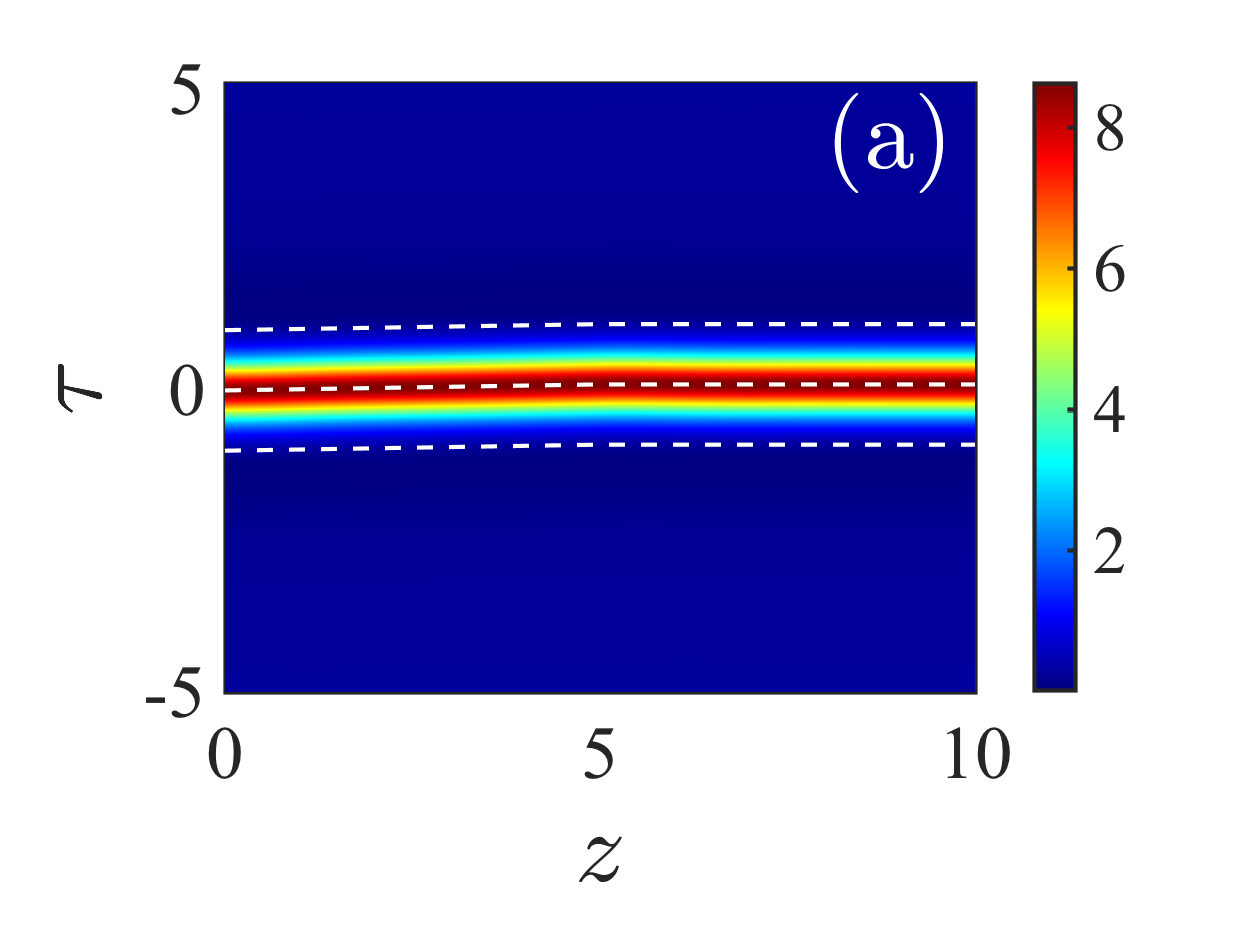
\includegraphics[width=\linewidth]{skinnyDensity1.eps} 
\caption{}
\end{subfigure}
\hspace{-1cm}
\begin{subfigure}{0.5\textwidth}
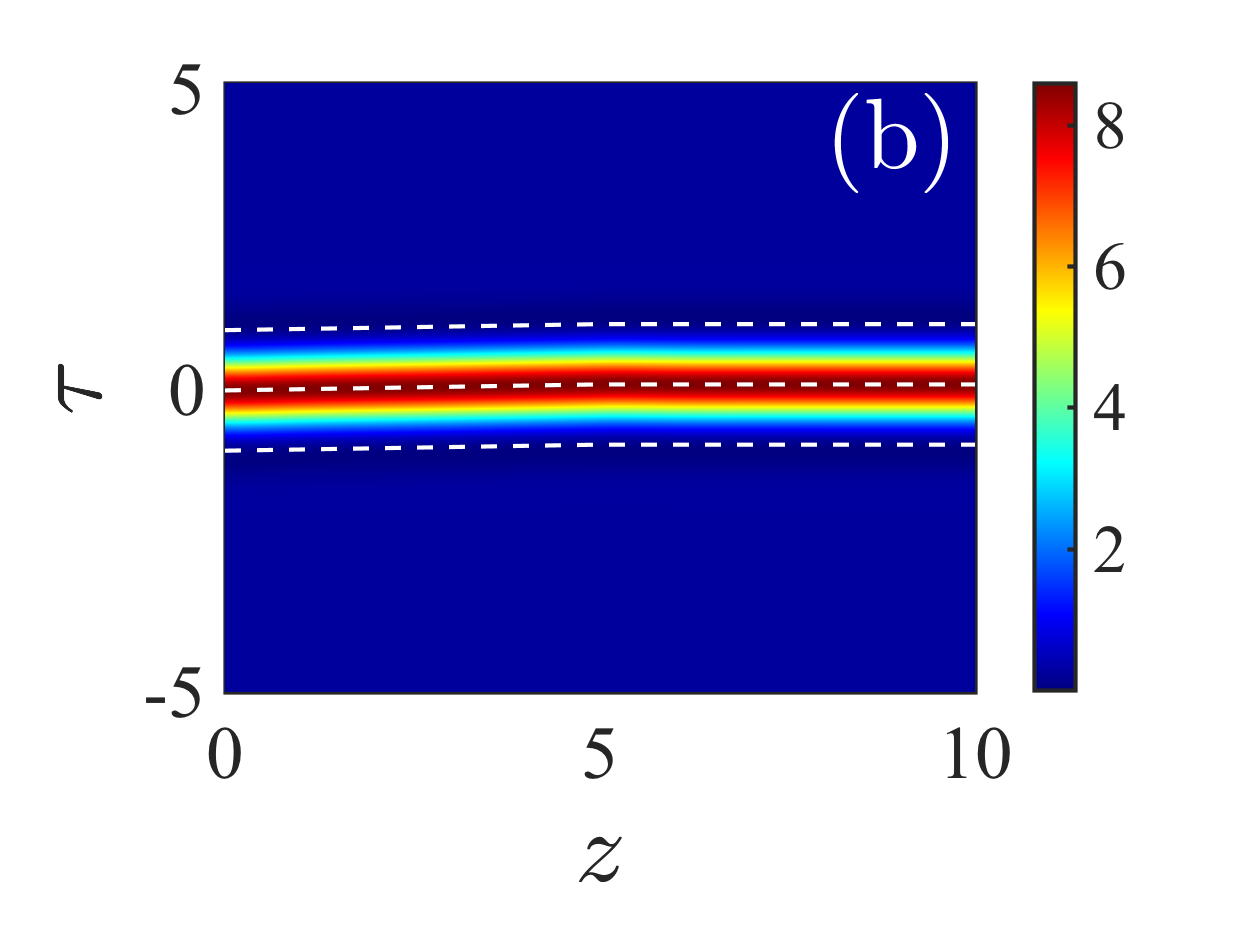
\includegraphics[width=\linewidth]{skinnyNCVADensity1.eps} 
\caption{}
\end{subfigure} }
\centerline{
\hspace{1cm}
\begin{subfigure}{\textwidth}
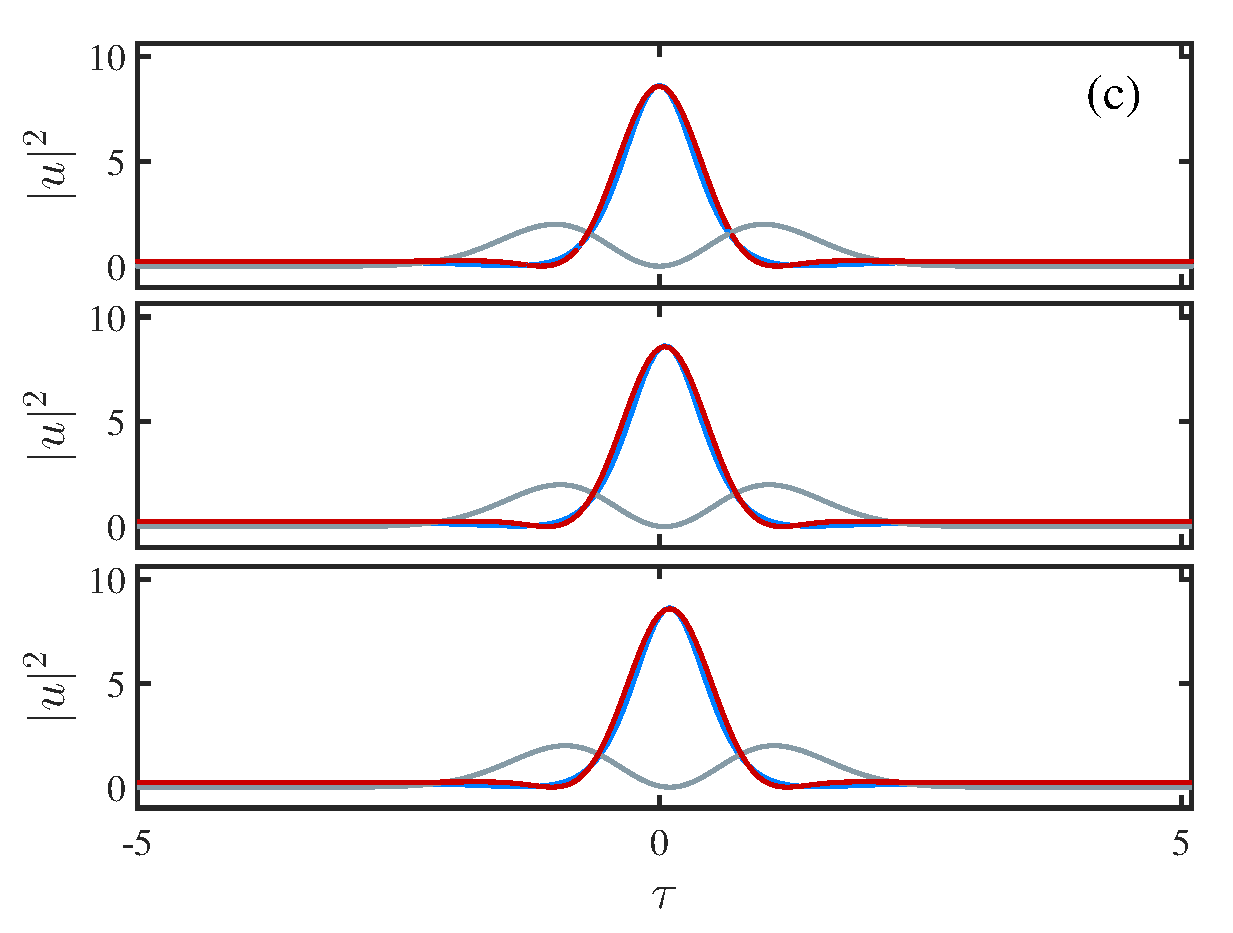
\includegraphics[width=0.9\linewidth]{skinnyTimeSeries1.eps} 
\caption{}
\end{subfigure}}
  \rule{35em}{0.5pt}
\caption[Dynamic Evolution of Narrow Tweezer with Tweezed CS]{Example of the density evolution for the narrow tweezer state with $\tau_f = 0.1$ and $\beta = 0.1$ for the LL model (a) and NCVA (b) and (c) snapshots for the corresponding states of LL model (solid (blue) line), NCVA (solid (red) line) and effective potential depicted as solid (grey) line.  Evolution of steady state CS solution in narrow tweezer for $\tau_0(z)$ (dashed (white) line) for full LL model (a) and NCVA (b).  The initial steady state, see LL model solid (blue) and NCVA solid (red) in top panel (c) for $z = 0$ and the state while being tweezed at $z = z^* = 2.5$ depicted in solid (blue) LL model [solid (red) NCVA] in middle panel (c).  The bottom panel (c) is the state at $z = z_f = 10$.  Both the density evolution in the LL model and NCVA, as well as the snapshots, correspond to a tweezed CS that is manipulated by the narrow tweezer. 
}
\label{fig:Skinny1}
\end{figure}

The NCVA solutions only have two fundamental states: (i) a tweezed CS or (ii) a no-CS solution (there is no NCVA solution in which the tweezer leaves behind a CS).  Therefore, it is not necessary to use $Q_{\rm O}$ since both states result in $Q_{\rm O} \approx 0$.  Figure~\ref{fig:SkinnyVsNCVA} depicts a single contour (white line) of the $Q_{\rm diff} = 0.5$ superimposed on the same density of the full LL model as in Fig.~\ref{fig:SkinnyQ}(c).  This figure allows for a direct comparison of the threshold between a tweezed CS and no-CS solution of the NCVA (white line) and the state regions of the full LL model.  For the narrow tweezer, the NCVA solutions have a wider region for the existence tweezed CS than the LL model.  The NCVA also has islands of tweezed CS for larger values of $\tau_f$ and $\beta$ which do not exist in the full LL model.

As a sample of the dynamic properties of tweezability, Fig.~\ref{fig:Skinny1} depicts a sample for a tweezed CS while Fig.~\ref{fig:Skinny2} depicts a dissipative no-CS solution for the full LL model.  Figs.~\ref{fig:Skinny1}(a) and~\ref{fig:Skinny1}(b) depict the dynamic evolution of the LL model and NCVA, respectively, for the narrow tweezer $\tau_f = 0.1$ and $\beta=0.1$.   Figure~\ref{fig:Skinny1}(c) contains three snapshots of the system at $z=0$ (top panel), $z^*$ (middle panel), and 10 (bottom panel) for comparison between the LL model (solid (blue) line), the NCVA solution (solid (red) line) and the tweezer (solid (grey) line).  For an example of no-CS dynamic properties, Fig.~\ref{fig:Skinny2} for narrow tweezer $\tau_f = 2$ and $\beta=10$ is organized the same as Fig.~\ref{fig:Skinny1}.   In this example, the NCVA and the LL model admits a no-CS state.  It is also important to mention that the NCVA variational parameters for the narrow tweezer accurately capture the full LL model solution properties, such as height and width as seen in Figs~\ref{fig:Skinny1}(c) and ~\ref{fig:Skinny2}(c).



\begin{figure}[htb!]
\centering
\centerline{
\hspace{1cm}
\begin{subfigure}{0.5\textwidth}
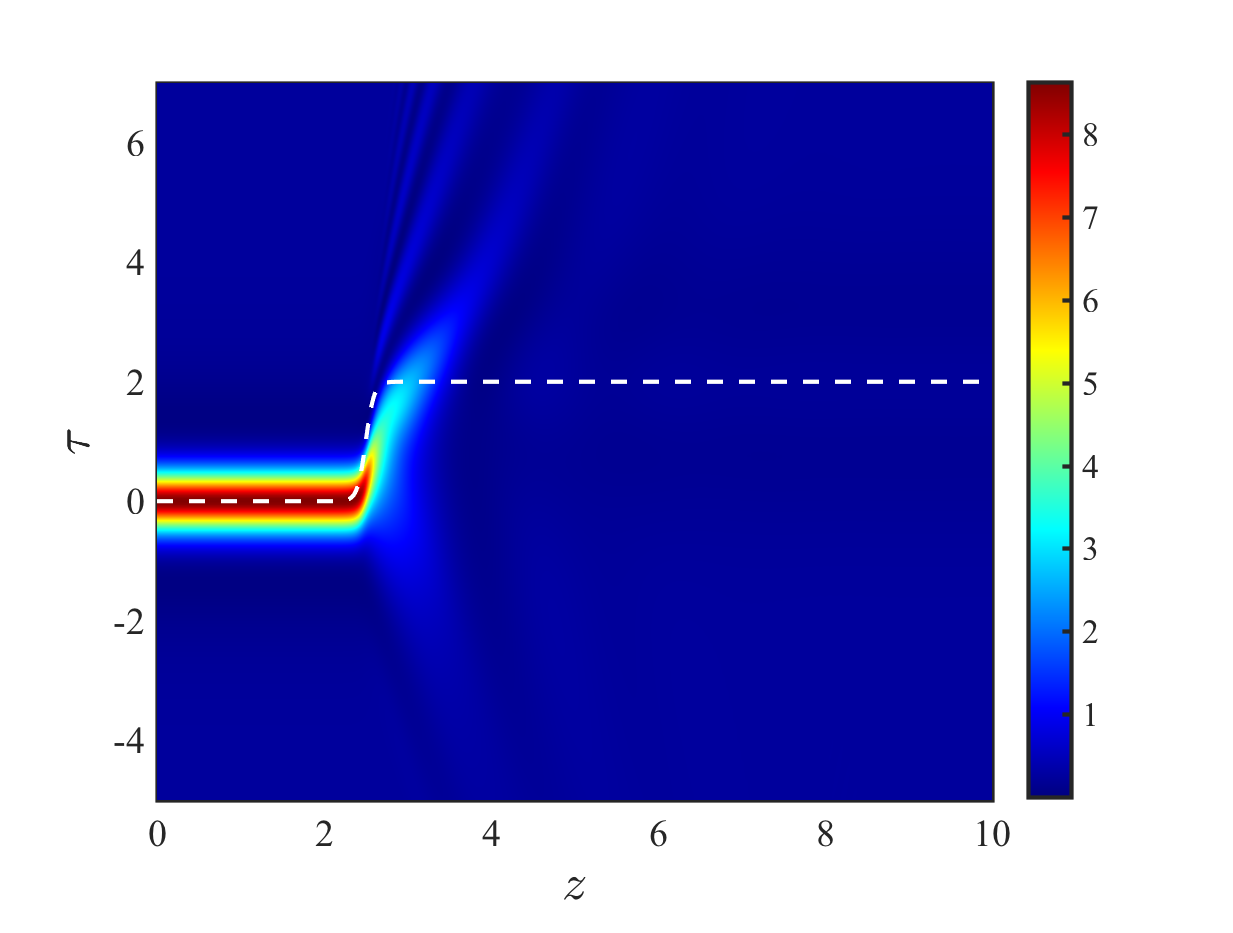
\includegraphics[width=\linewidth]{skinnyDensity3.eps} 
\caption{}
\end{subfigure}
\hspace{-1cm}
\begin{subfigure}{0.5\textwidth}
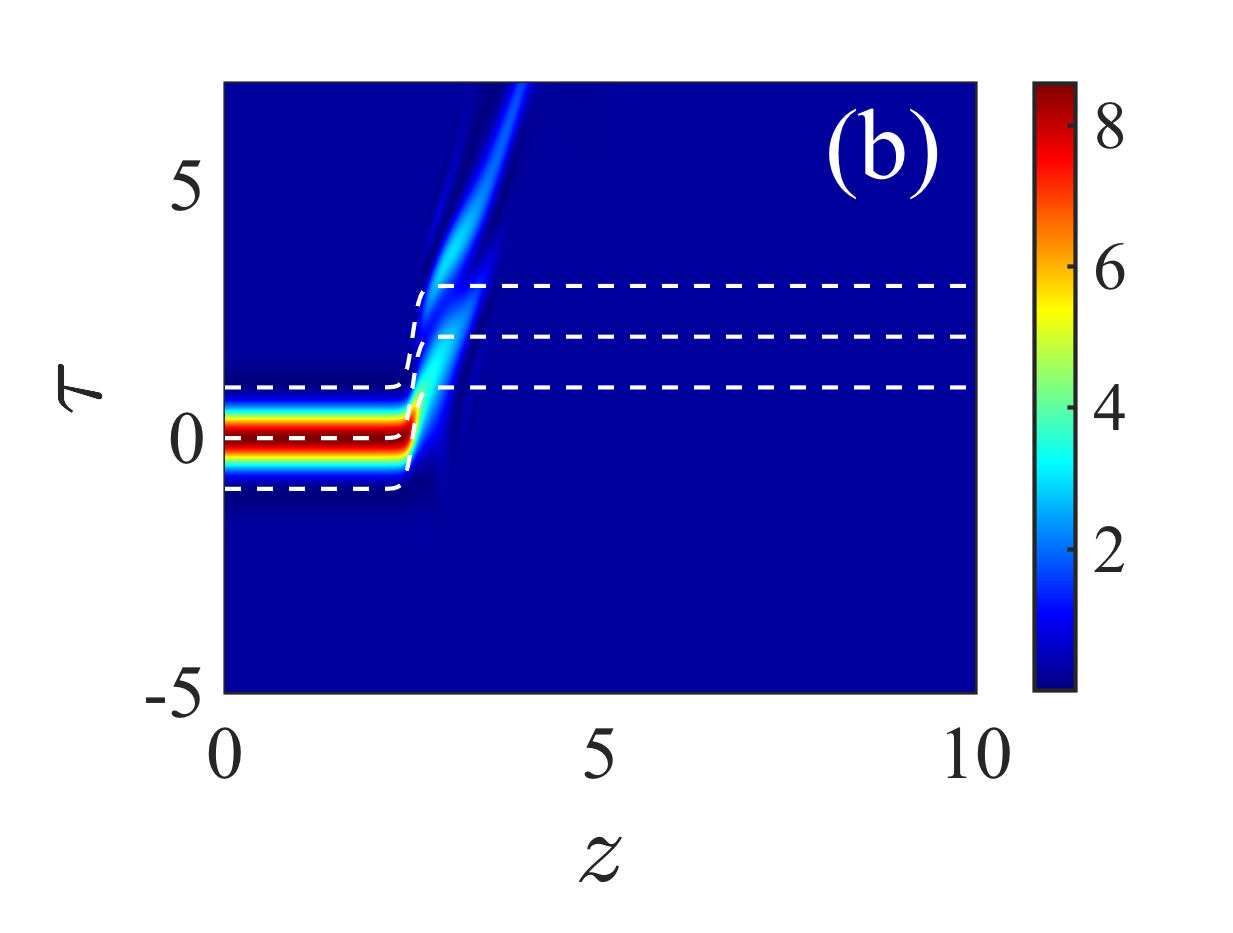
\includegraphics[width=\linewidth]{skinnyNCVADensity3.eps} 
\caption{}
\end{subfigure} }
\centerline{
\hspace{1cm}
\begin{subfigure}{\textwidth}
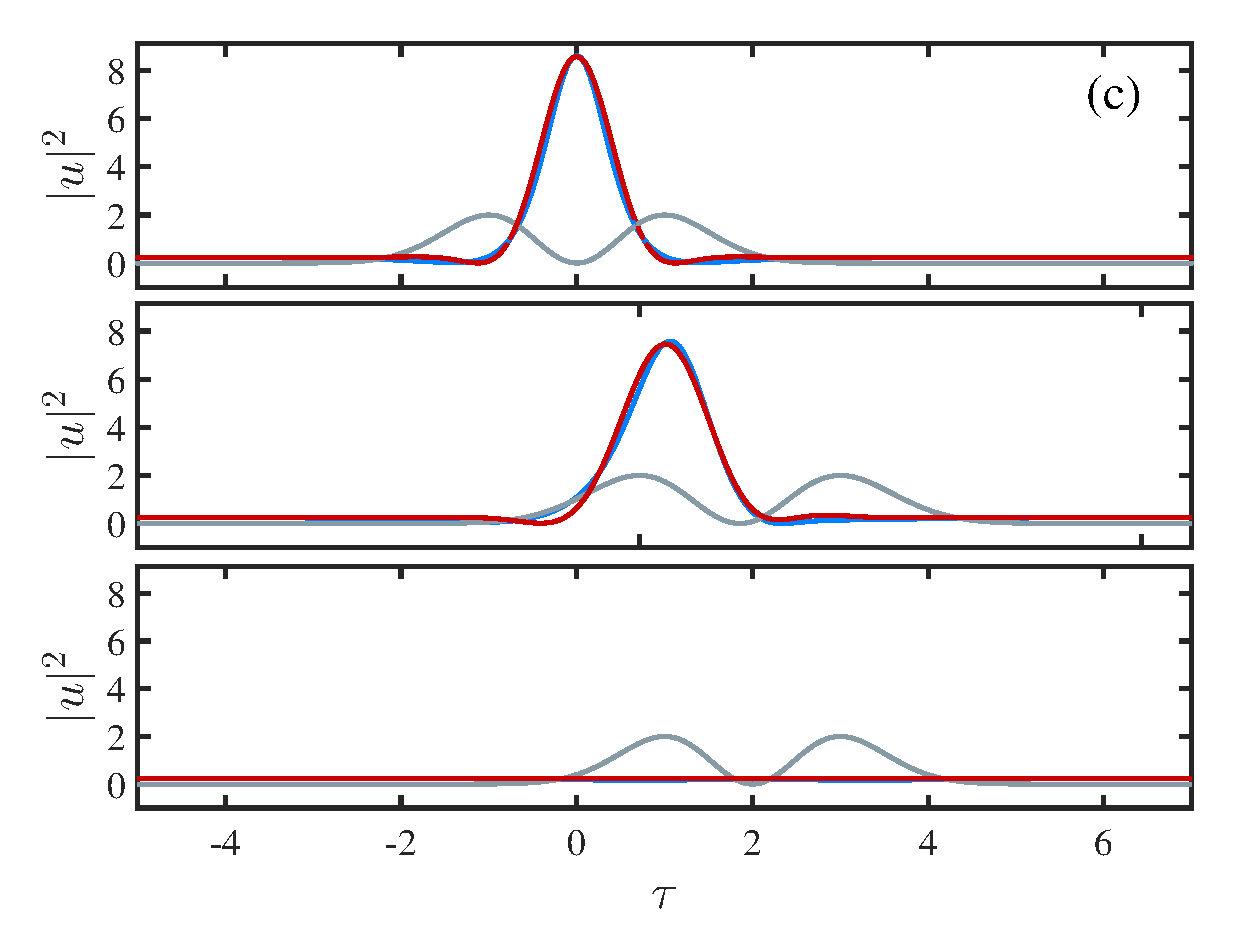
\includegraphics[width=0.9\linewidth]{skinnyTimeSeries3.eps} 
\caption{}
\end{subfigure}}
 \rule{35em}{0.5pt}
\caption[Dynamic Evolution of Narrow Tweezer with no-CS]{Dynamic evolution as in Fig.~\ref{fig:Skinny1} but for $\tau_f = 2$ and $\beta = 10$.  Same layout as in Fig.~\ref{fig:Skinny1}.  In this sample, both the LL model solution and NCVA are a no-CS.
}
\label{fig:Skinny2}
\end{figure}




\clearpage

\setstretch{1.3}
\subsection[Tweezer with Natural Width]{Tweezer with Natural Width} \label{section:Regular}
\setstretch{2}

In the second case study, we are interested in a tweezer with a natural width $\sigma_\phi = 2$ and height $h_\phi = 4.6633$ by Eq.~(\ref{height}).  %For the full LL Eq.~(\ref{eq:LLETweeze}), the steady state CS is found centered at $\tau_0 = 0$ using a Newton-Krylov solver and 
The power-balance constraint Eq.~(\ref{LLConstraint}) selects a detuning parameter $\Delta =  2.8357$ for this system.  The same $\Delta$, $\sigma_\phi$, and $h_\phi$ are used in the NCVA with a Newton-Krylov solver to find the initial parameters for the system.  The parameter space for $\beta$ and $\tau_f$ are discretized as in Sec.~\ref{section:Skinny}.  %The NCVA and full LL Eq.~(\ref{eq:LLETweeze}) are solved with the same methods described above. 
%Again, the full LL Eq.~(\ref{eq:LLETweeze}) is solved using Runge-Kutta methods and the NCVA system of ODEs are solved using Matlab's ode15s.  Both the full LL equation and NCVA are allowed to evolve until $z_f = 10 = 4z^*$ with $z^* = 2.5$.

\begin{figure}[p]
\centering 
\hspace{0cm}
\begin{subfigure}{0.5\textwidth}
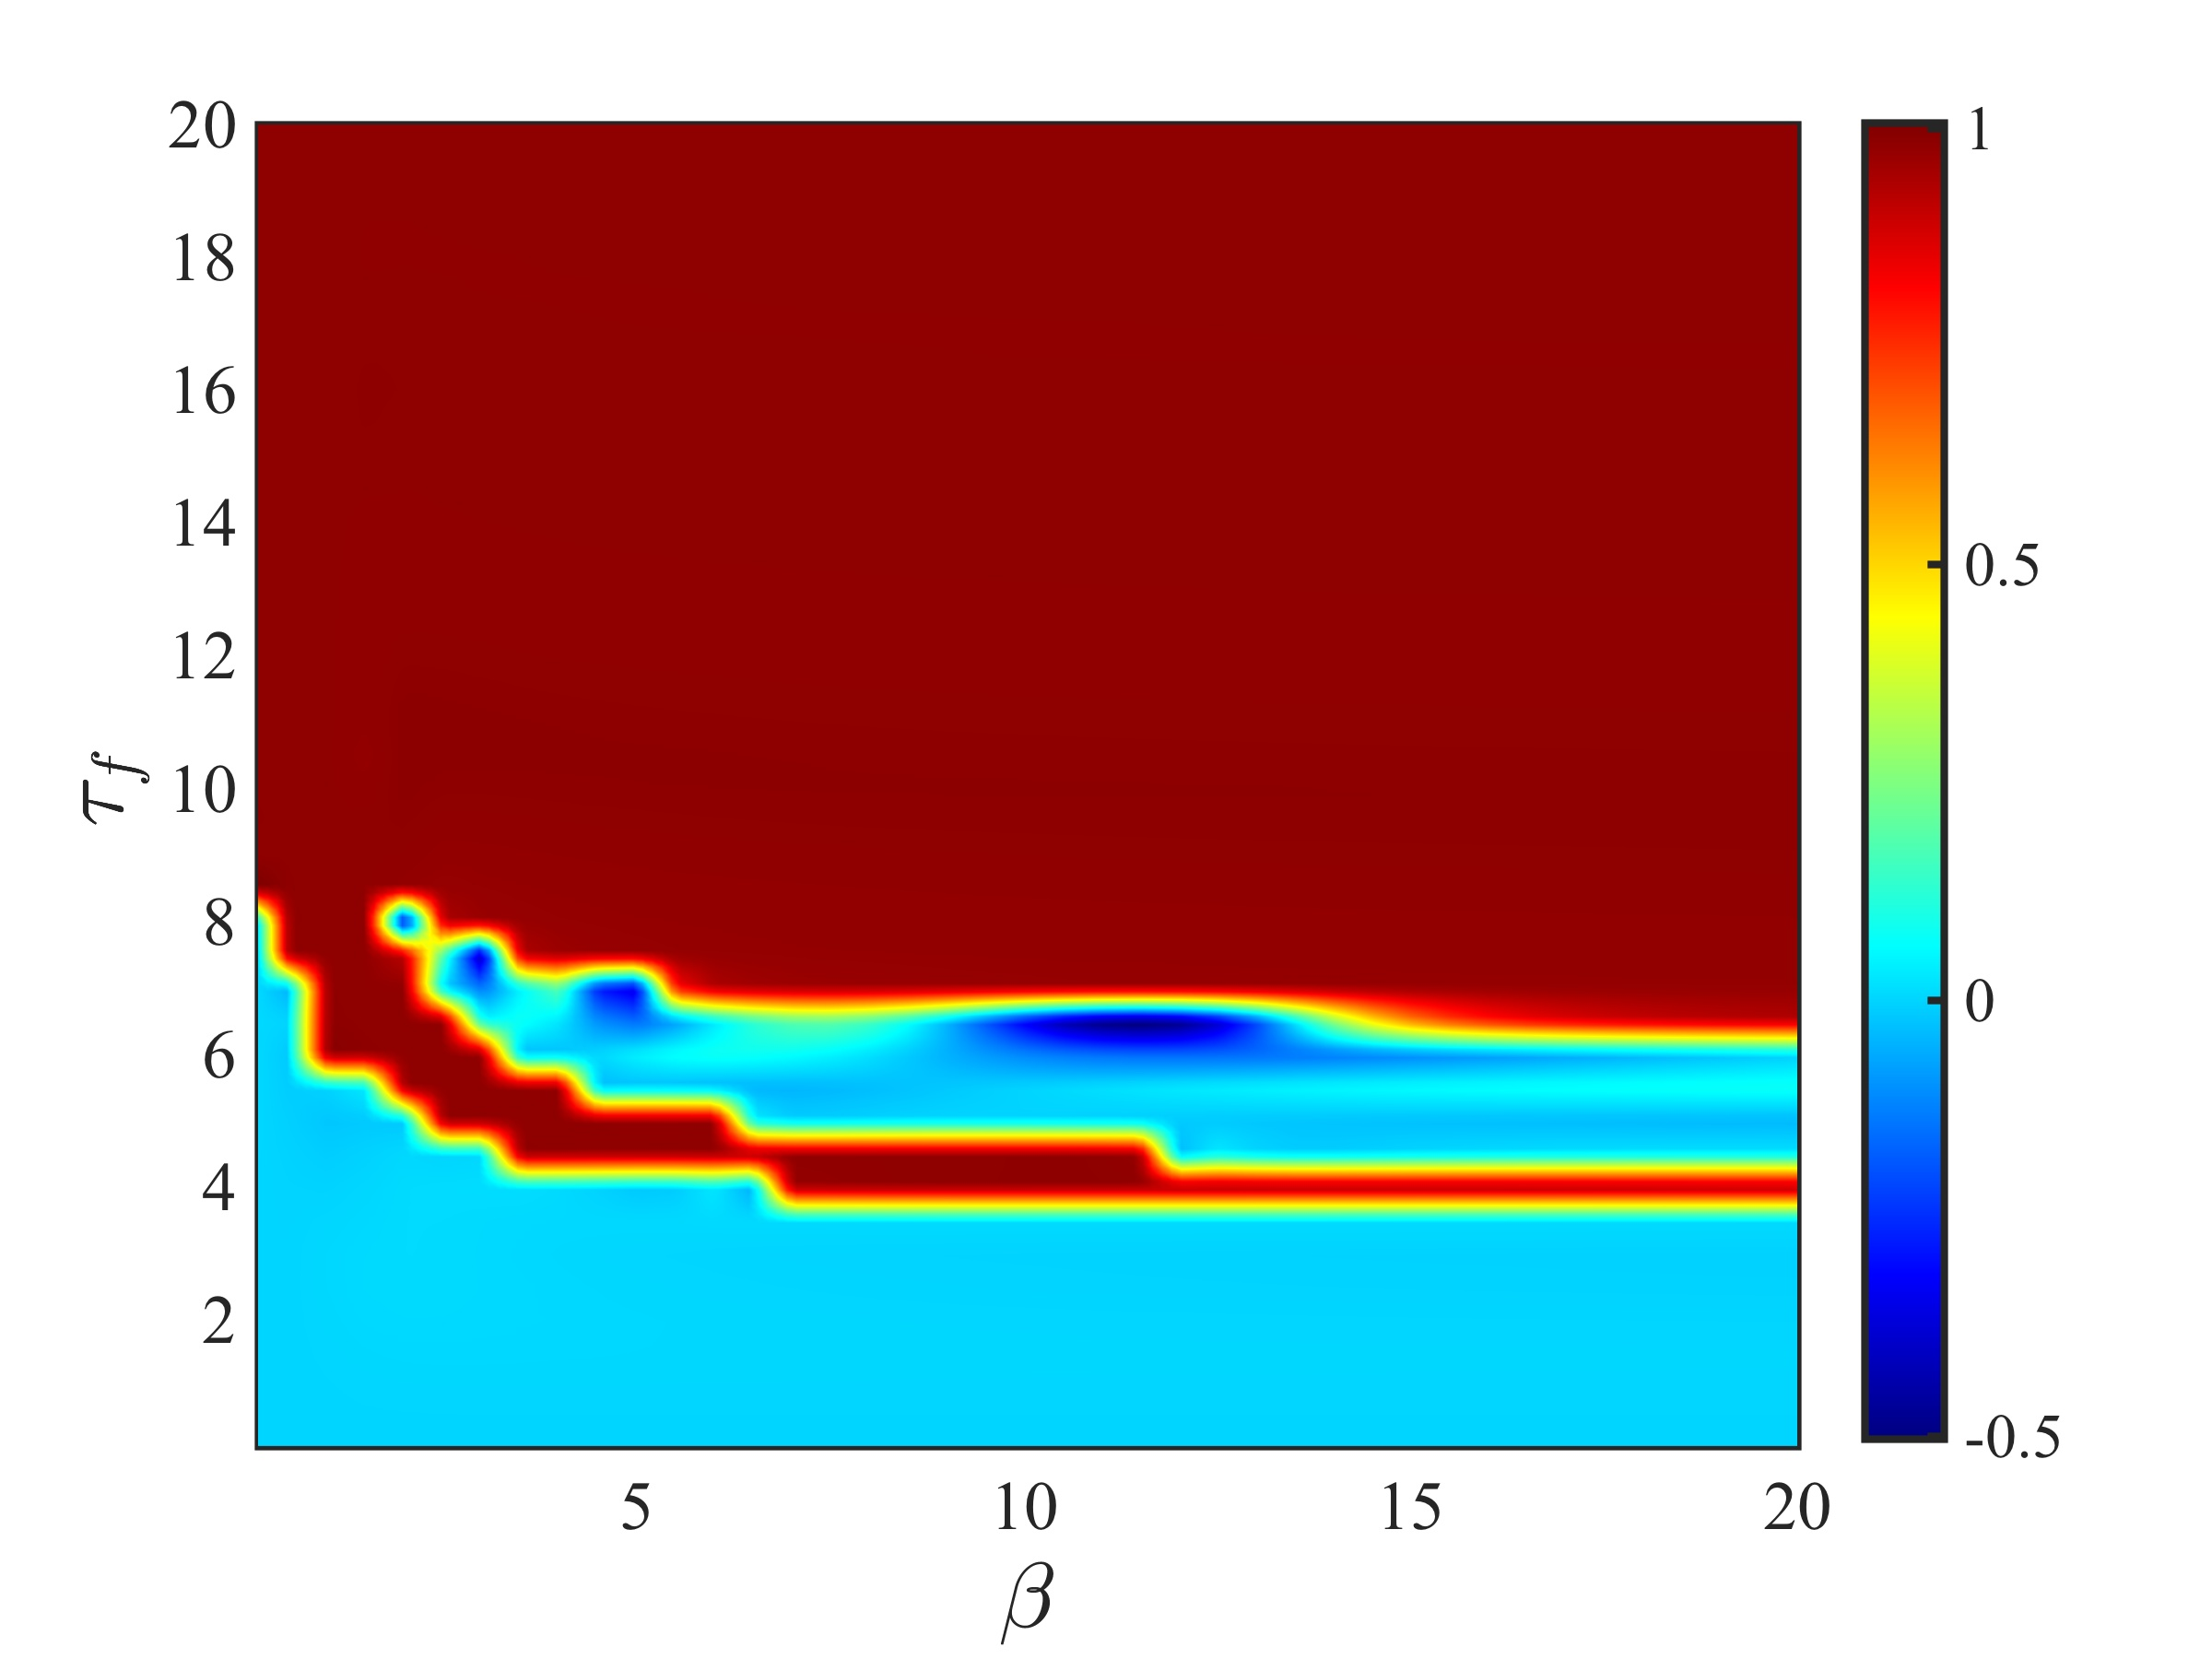
\includegraphics[width=\linewidth]{RegularQIn.jpg}
\caption{} 
\end{subfigure}
%\hspace*{\fill}
\hspace*{-0.5cm}
\begin{subfigure}{0.5\textwidth}
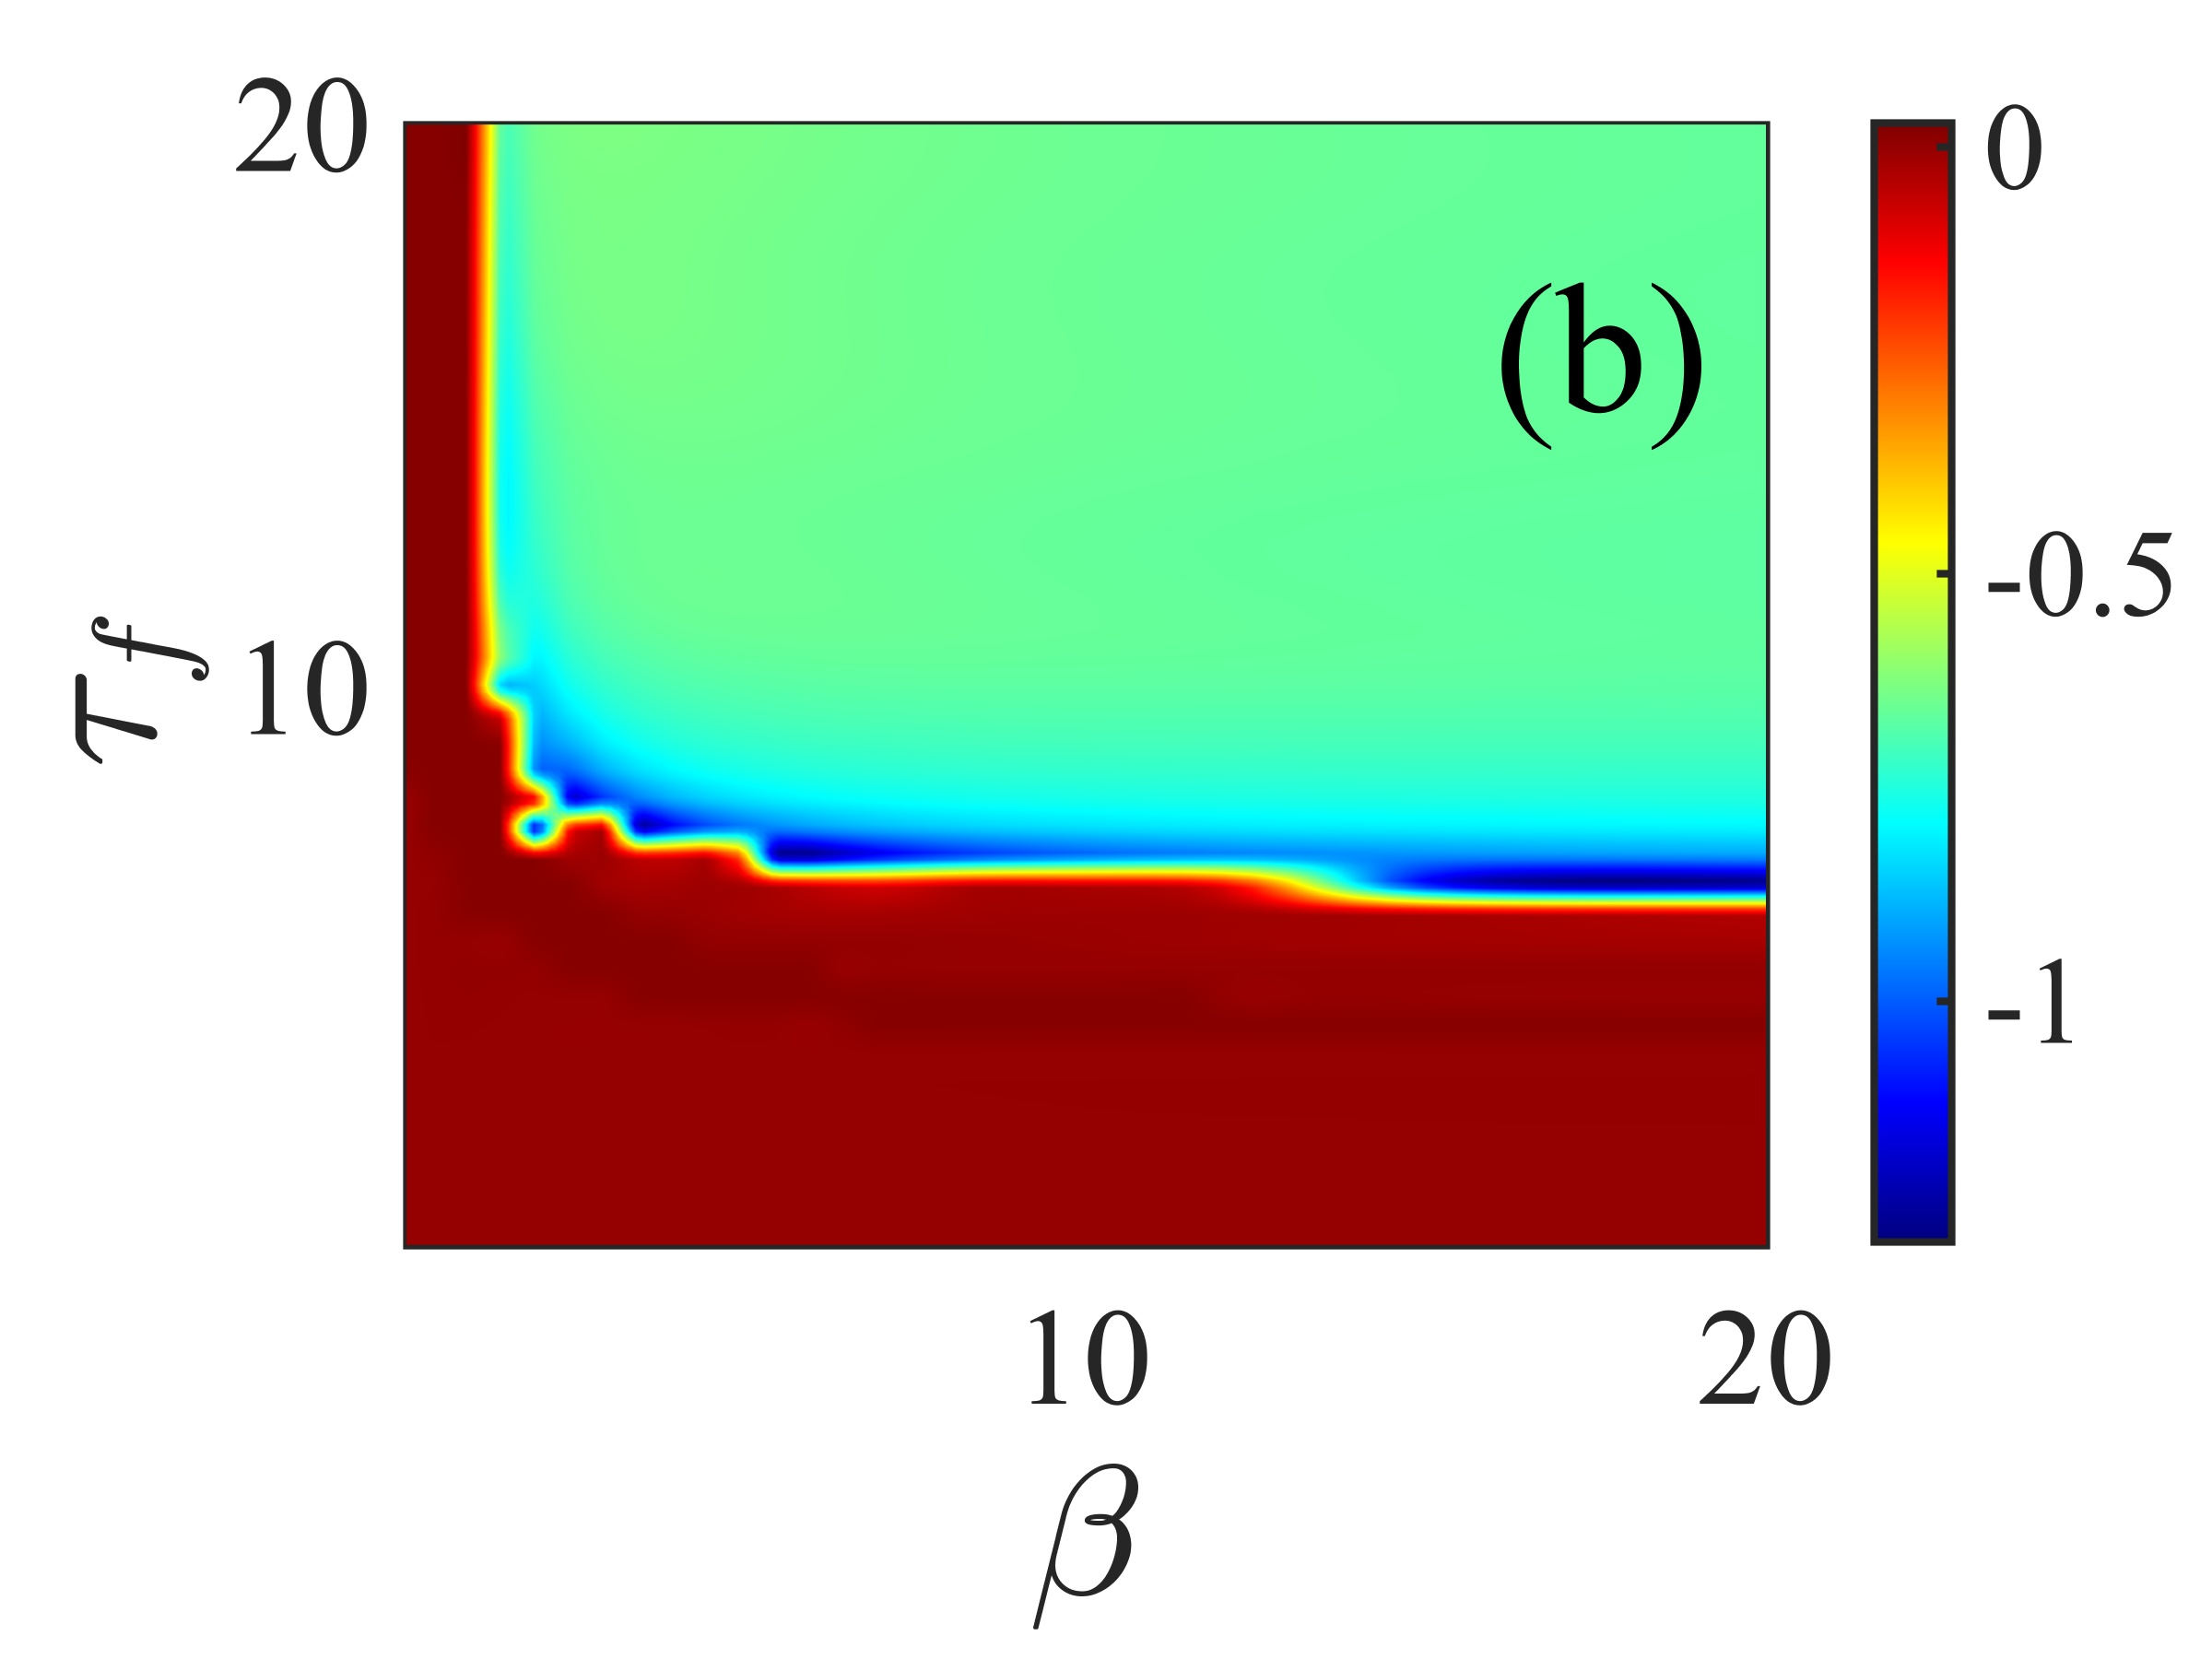
\includegraphics[width=\linewidth]{RegularQOut.jpg} 
\caption{} 
\end{subfigure} 
\centerline{
%\hspace{1cm}
\begin{subfigure}{\textwidth}
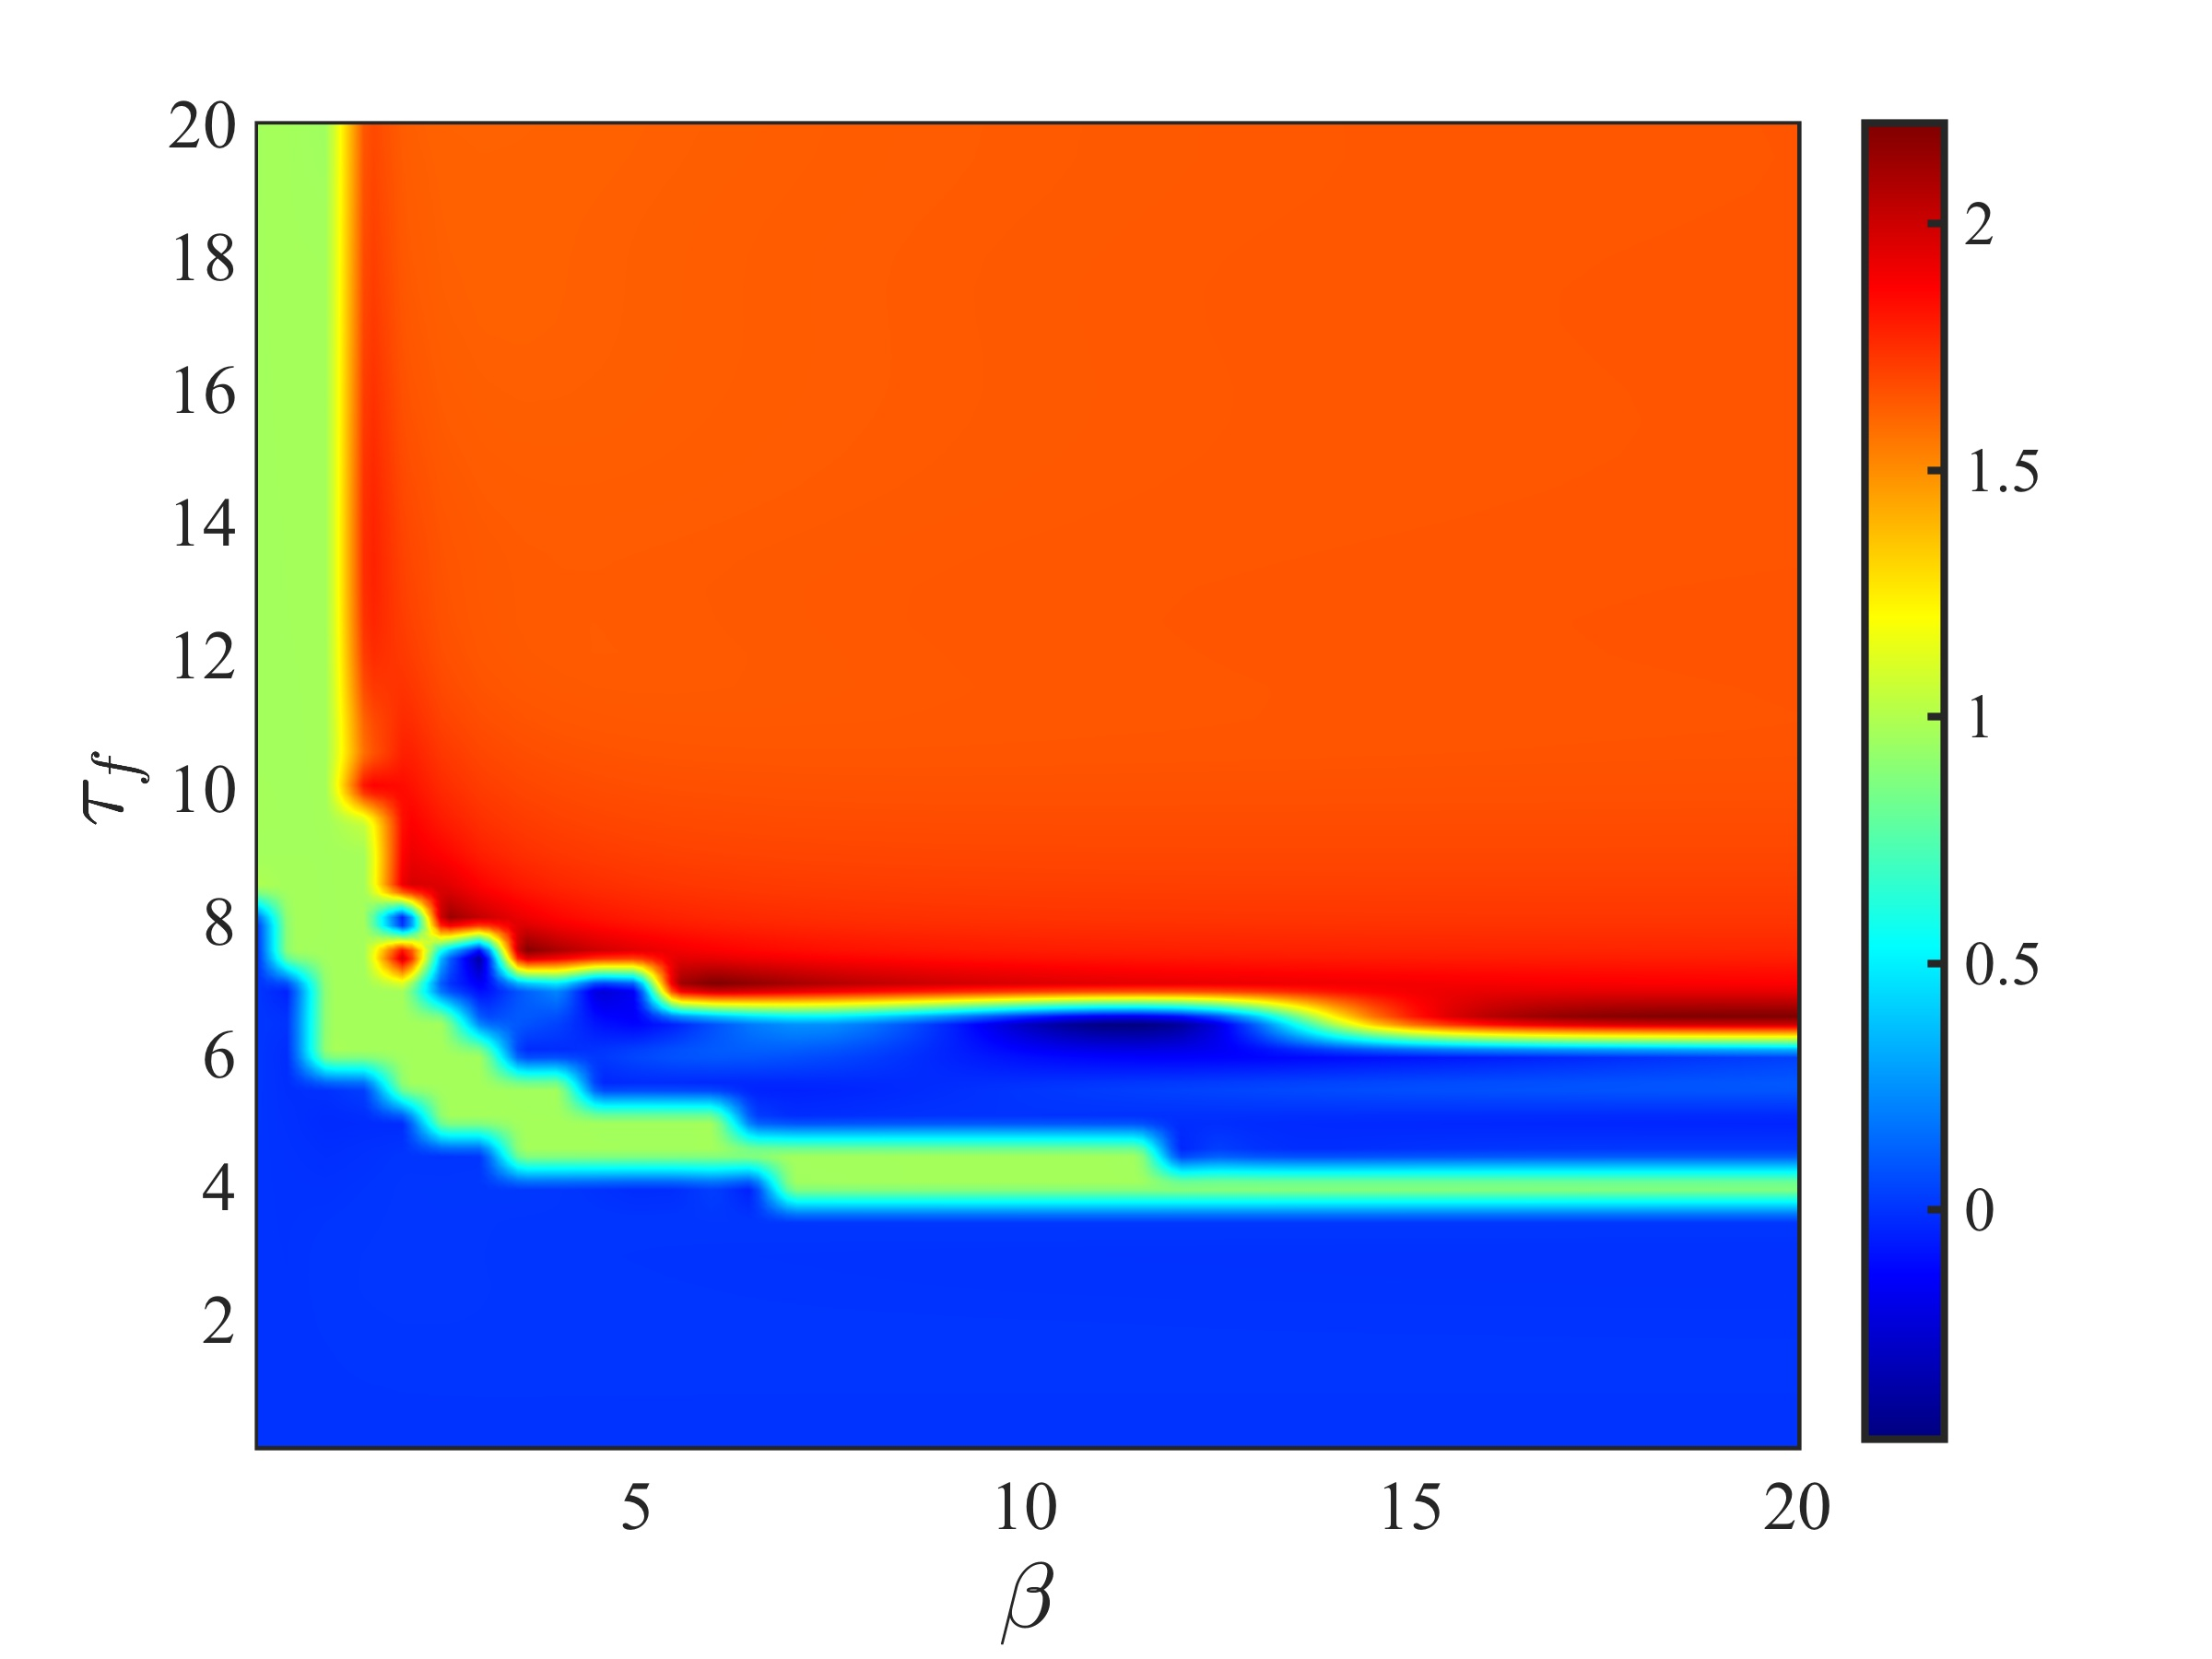
\includegraphics[width=\linewidth]{RegularQDiff.jpg} 
\caption{} 
\end{subfigure} }
  \rule{35em}{0.5pt}
\caption[Power Ratios Inside and Outside Tweezer with Natural Width]{Power ratios as in Fig.~\ref{fig:SkinnyQ} but for a natural tweezer with width $\sigma_\phi = 2$ and height $h_\phi = 4.6633$.  The detuning for the system is $\Delta =  2.8357$.   Same layout as in Fig.~\ref{fig:SkinnyQ}.  The difference power ratio (c) defines the thresholds for a tweezed CS for blue region below green region, a no-CS for all green regions, and non-tweezed for for all orange regions.  
}
\label{fig:RegularQ}
\end{figure}

\begin{figure}[htb!]
\centering
\centerline{
\begin{subfigure}{0.5\textwidth}
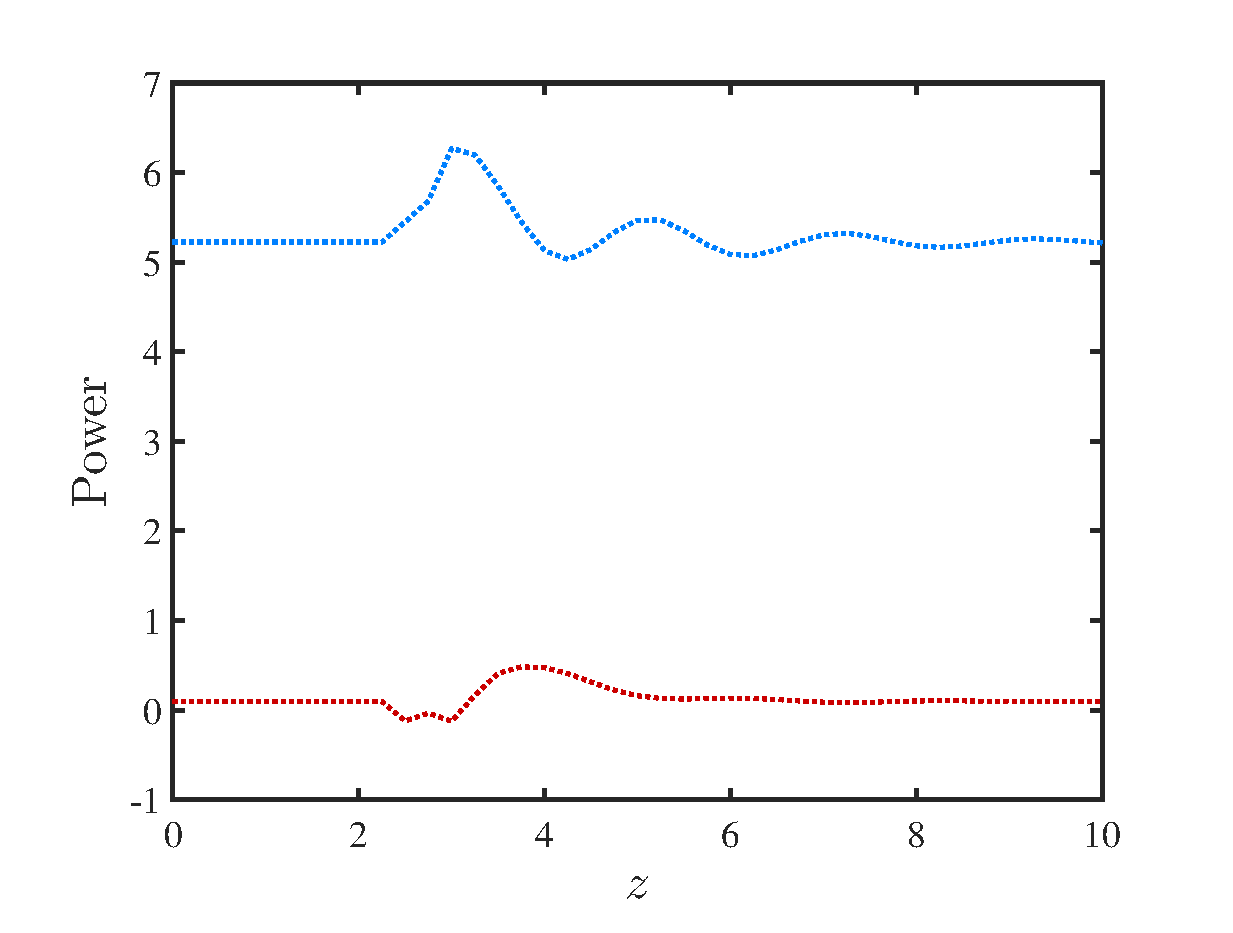
\includegraphics[width=\linewidth]{regularTimeMass1.eps} 
\caption{}
\end{subfigure}
\begin{subfigure}{0.5\textwidth}
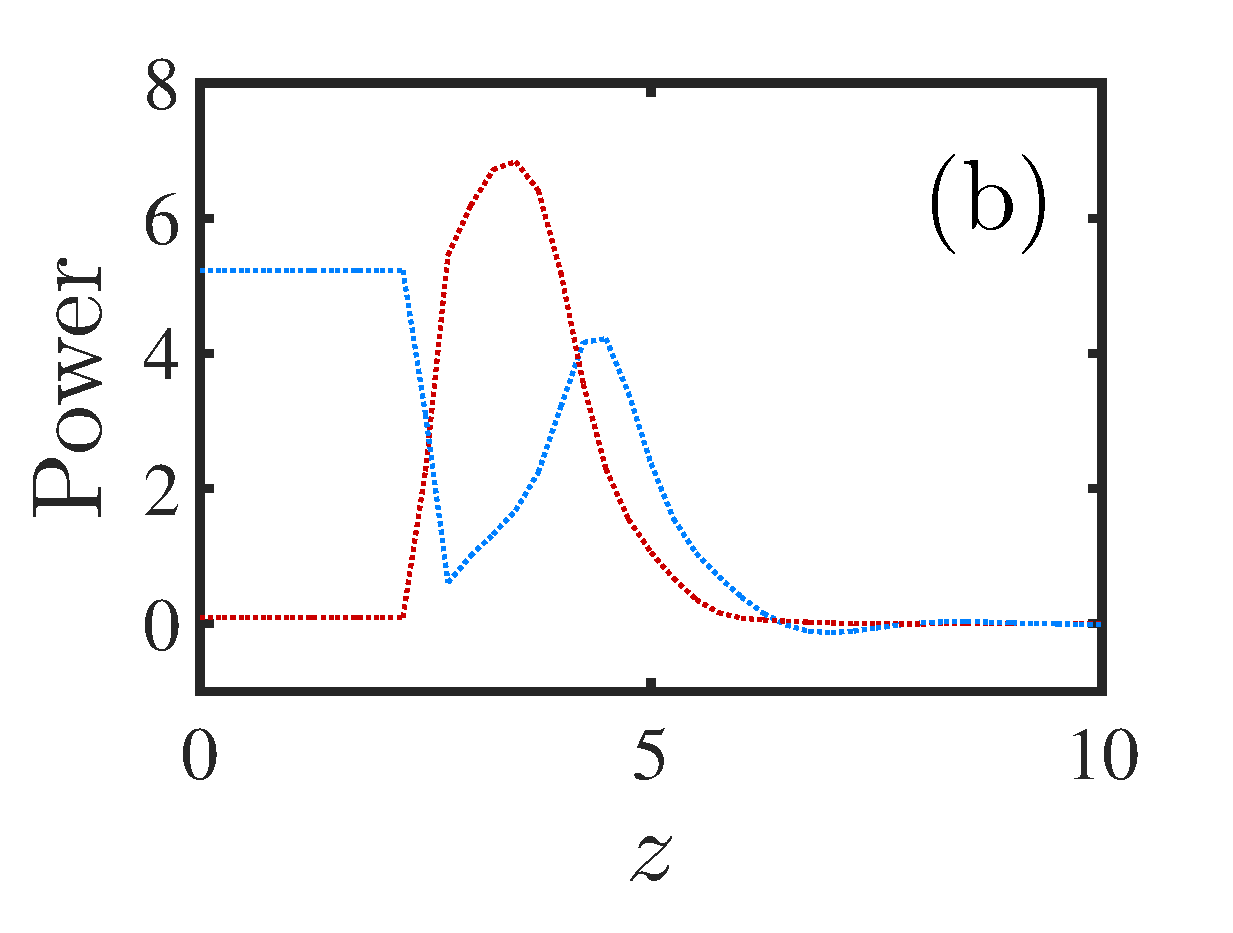
\includegraphics[width=\linewidth]{regularTimeMass5.eps} 
\caption{}
\end{subfigure} }
\centerline{\begin{subfigure}{0.5\textwidth}
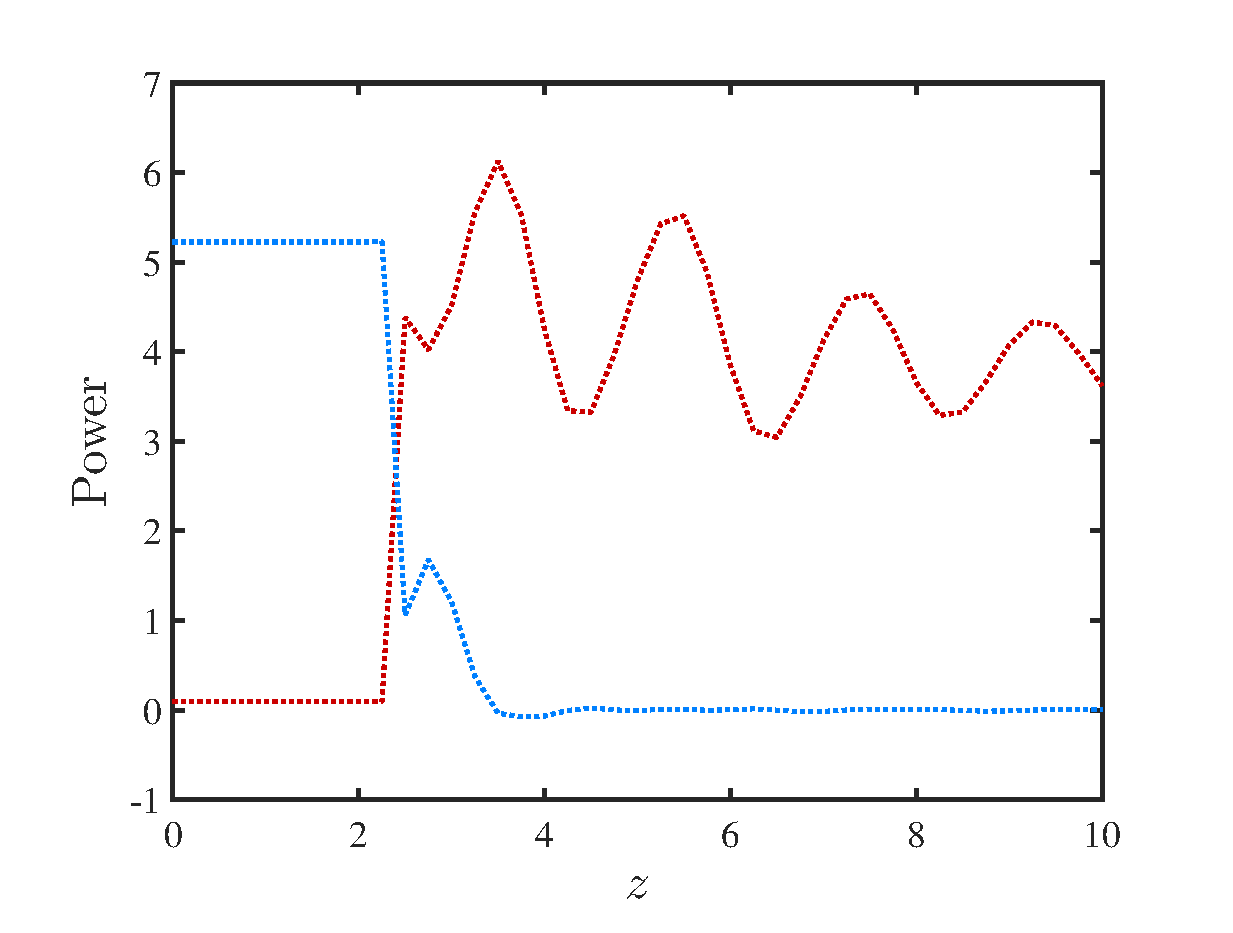
\includegraphics[width=\linewidth]{regularTimeMass3.eps} 
\caption{}
\end{subfigure} 
\begin{subfigure}{0.5\textwidth}
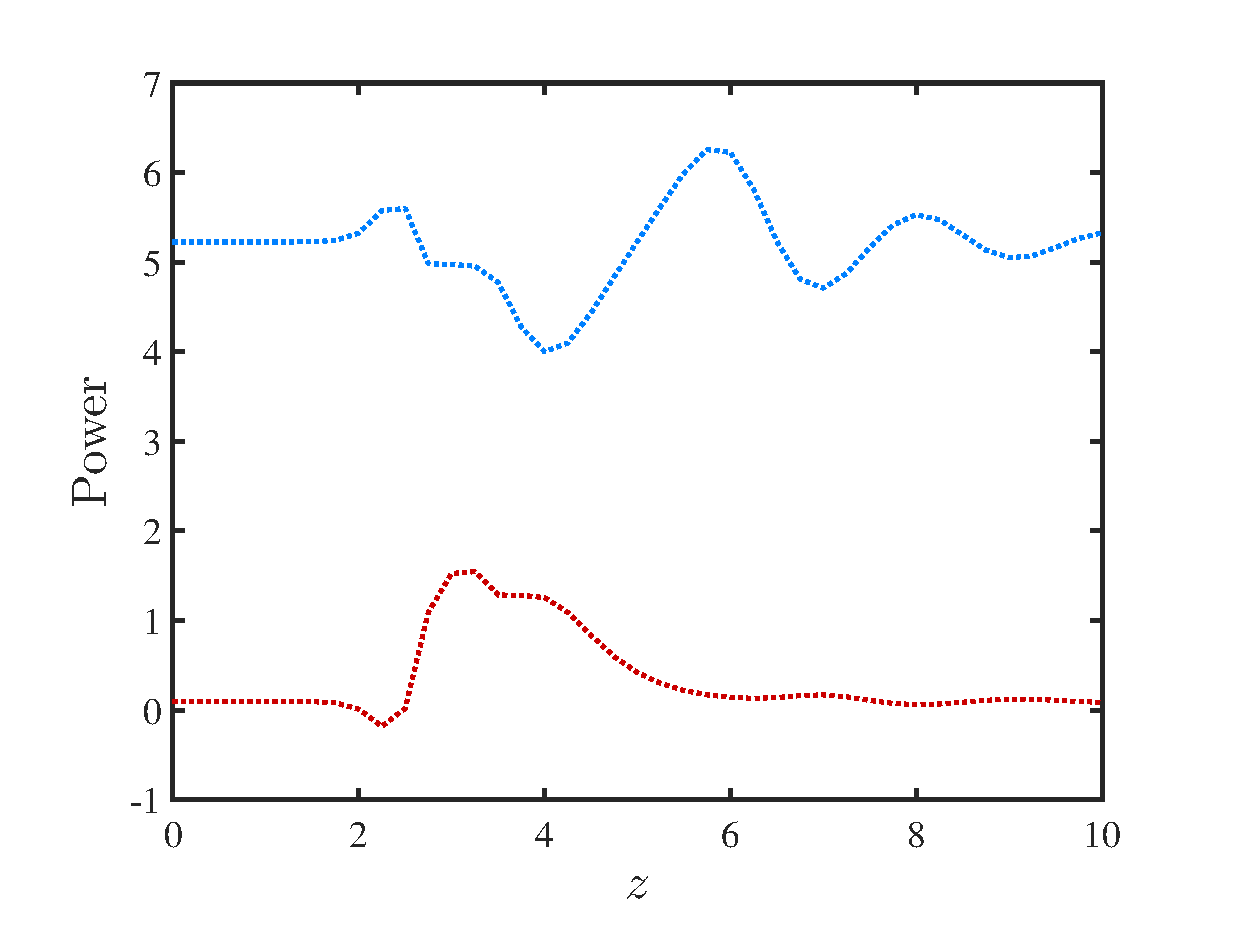
\includegraphics[width=\linewidth]{regularTimeMass4.eps}
\caption{}
\end{subfigure} } 
 \rule{35em}{0.5pt}
\caption[Tweezer with Natural Width Power Comparison]{Comparison of the powers as in Fig.~\ref{fig:SkinnyComp} but for a natural tweezer.  Same layout as Fig.~\ref{fig:SkinnyComp}, but for parameters (a) $\tau_f = 2$ and $\beta=10$, (b) $\tau_f = 4.5$ and $\beta=10$, (c) $\tau_f = 12$ and $\beta=10$ and (d) $\tau_f = 5$ and $\beta=2$.  The left top panel (a) has no change in power inside or outside the tweezer which describes a tweezed CS, while right top panel (b) shows power change for no-CS.  The left bottom panel (c) is an example of the tweezer moving too quickly and leaving the CS outside the tweezer (non-tweezed).  The right bottom panel (d) is again a tweezed-CS.
}
\label{fig:RegularComp}
\end{figure}

\begin{figure}[htb!]
\centering
\centerline{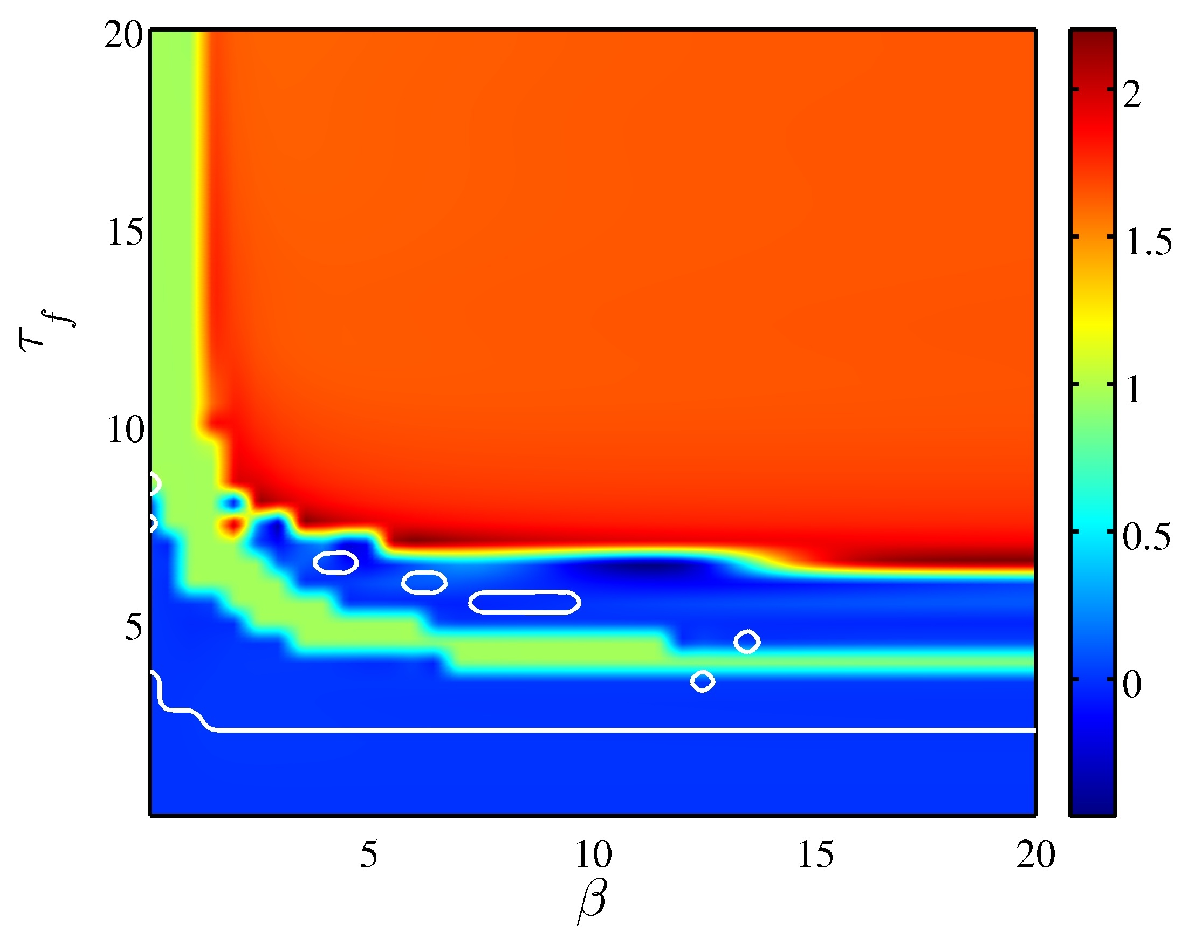
\includegraphics[width=0.9\textwidth]{RegularPDEvODE_rcg_t.eps}}
  \rule{35em}{0.5pt}
\caption[Comparison of Power Ratios of Natural Tweezer for LL Model and NCVA]{Comparison of difference in power ratios between the NCVA and LL model as in Fig.~\ref{fig:SkinnyVsNCVA} but for a natural tweezer.  Same layout as Fig.~\ref{fig:SkinnyVsNCVA}.  The NCVA distinguishes a threshold between tweezed and no-CS soltions at $\approx 2.5$ and regions of tweezed CS for larger parameters.  The LL model has clear regions of state, namely, a tweezed CS in blue region (under the green region), no-CS in the green region, and a non-tweezed CS in orange region.
}
\label{fig:RegularVsNCVA}
\end{figure}

As described in the previous section, we calculate $Q_{\rm I}$ from Eq.~(\ref{QIn}) and $Q_{\rm O}$ from Eq.~(\ref{QOut}) for all parameter combinations.  Figure~\ref{fig:RegularQ} depicts the density of these power ratios inside (Fig.~\ref{fig:RegularQ}(a)) and outside (Fig.~\ref{fig:RegularQ}(b)) the natural tweezer.  The $Q_{\rm diff}$ in Fig.~\ref{fig:RegularQ}(c) clearly defines three fundamental states: a tweezed CS for all $\beta$ when $\tau_f < 4$ (blue region), no-CS (green region), and a non-tweezed CS (orange/red regions).  Please note that the blue region between the green and orange regions in Fig.~\ref{fig:RegularQ}(c) is ``artificial'' tweezing (an example is given in Sec.~\ref{section:Fat}).  In this region, the tweezer initially drags the CS but the CS is eventually left behind by the trap; however, the CS remains in motion and catches up to the trap by $z = z_f$, and the CS reenters the trap at $\tau_f$ which is measured in our power quotient.  The threshold for the existence of the tweezed CS with a natural tweezer is larger than we found for a narrow tweezer and occurs at $\tau_f \approx 4$.

In order to better explain the power ratio, we examine four examples of the power inside $P_{\rm I}$ Eq.~(\ref{Pin}) and outside $P_{\rm O}$ Eq.~(\ref{Pout}) for $\beta = 10$ at $\tau_f = 2$, 4.5, and 12 as well as $\beta = 2$ and $\tau_f = 5$ in Fig.~\ref{fig:RegularComp}.  According to Fig.~\ref{fig:RegularQ}, for the example with $\tau_f = 2$ and $\beta=10$ we have a tweezed CS and for $\tau_f=4.5$ and $\beta = 10$ we have no-CS.   By analyzing the power as a function of $z$ we can follow the evolution of the system.  In Fig.~\ref{fig:RegularComp} the red lines correspond to $P_{\rm I}$ and the blue lines to $P_{\rm O}$.  Figure~\ref{fig:RegularComp}(a), with parameters $\beta = 10$ and $\tau_f = 2$, there is no considerable change in power inside or outside the tweezer which describes a tweezed CS, while Fig.~\ref{fig:RegularComp}(b) corresponds to a loss of all mass inside (and outside) the trap which describes a no-CS.  Figure~\ref{fig:RegularComp}(c), with parameters $\beta = 10$ and $\tau_f = 12$, is an example of the tweezer moving too quickly and leaving the CS behind outside the tweezer (a non-tweezed CS).  Figure~\ref{fig:RegularComp}(d), with parameters $\beta = 2$ and $\tau_f = 5$, shows relatively little change in power inside or outside, which again is a tweezed CS.

Using the same layout as Fig.~\ref{fig:SkinnyVsNCVA}, Fig.~\ref{fig:RegularVsNCVA} compares the difference in quotient ratios between the NCVA and the full LL model.  The NCVA threshold between the tweezed CS and no-CS is approximately $\tau_f = 2.5$ while the LL model has a threshold around $\tau_f = 4$ for most $\beta$.  In addition to the threshold, the NCVA also has islands of regions for tweezed CS for larger $\tau_f$ and $\beta$ parameters.  These islands are capturing additional NCVA dynamic that are in agreement with the blue regions of the LL model.

\begin{figure}[htb!]
\centering
\centerline{
\hspace{1cm}
\begin{subfigure}{0.5\textwidth}
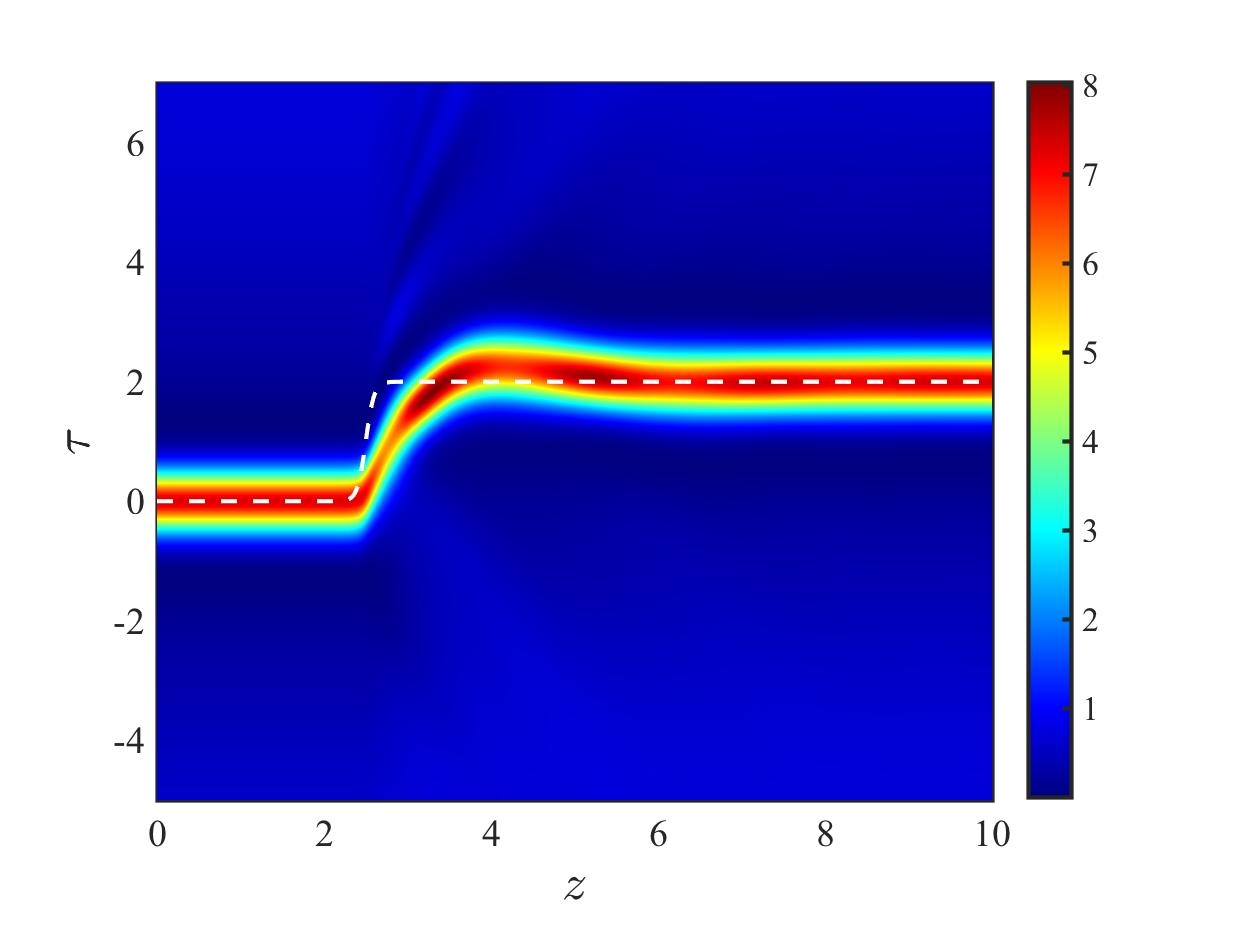
\includegraphics[width=\linewidth]{regularDensity1.eps} 
\caption{}
\end{subfigure}
\hspace{-1cm}
\begin{subfigure}{0.5\textwidth}
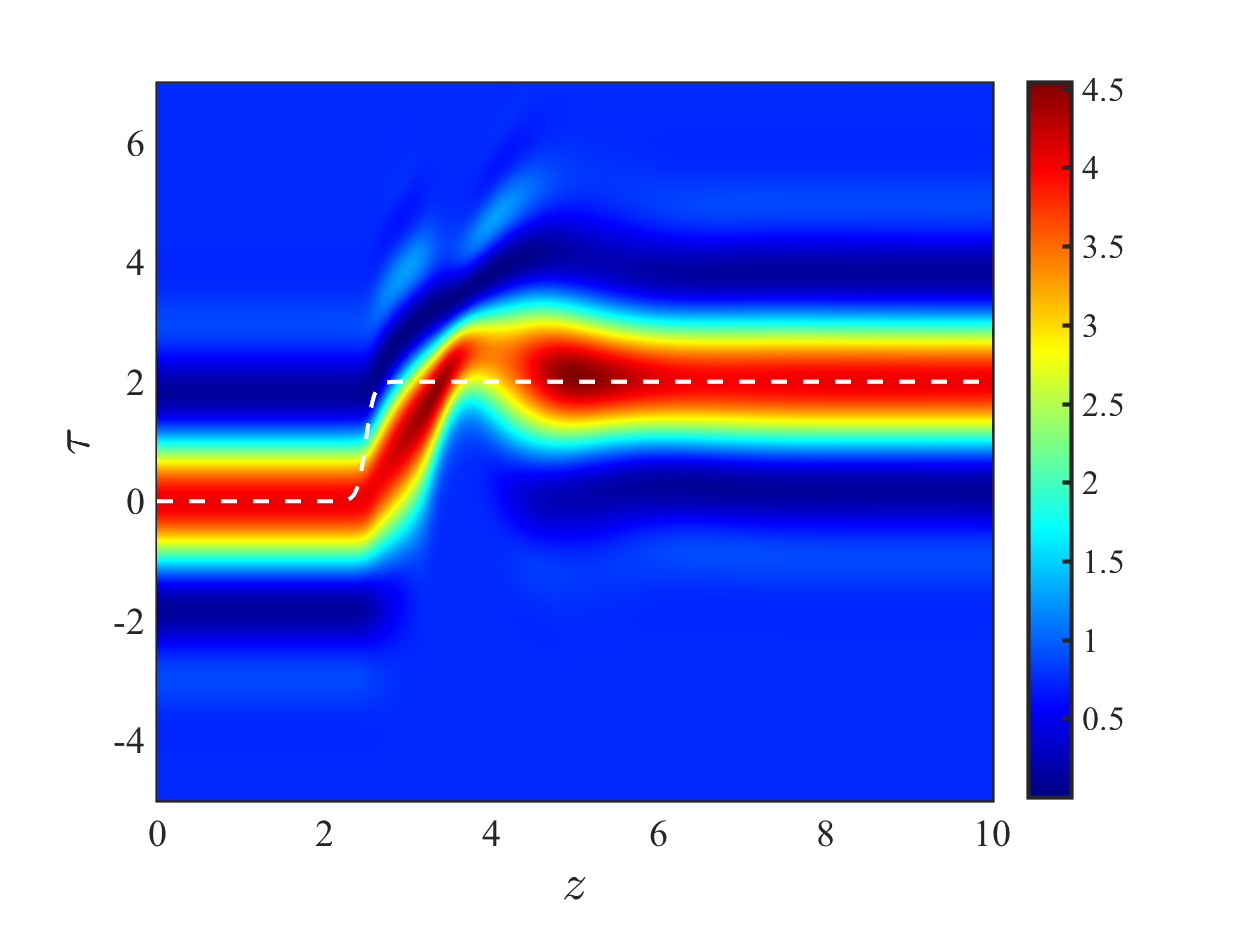
\includegraphics[width=\linewidth]{regularNCVADensity1.eps} 
\caption{}
\end{subfigure} }
\centerline{
\hspace{1cm}
\begin{subfigure}{\textwidth}
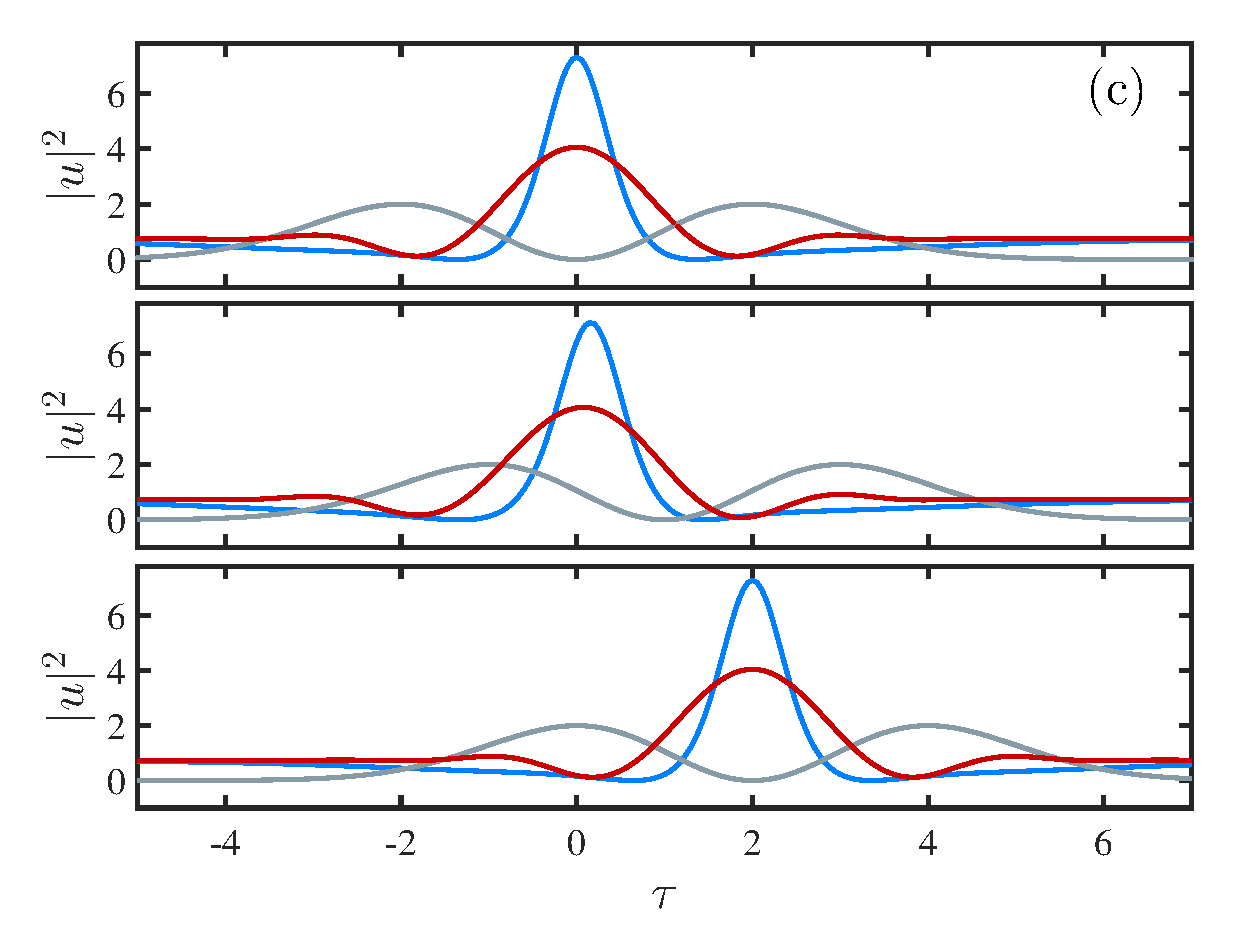
\includegraphics[width=0.9\linewidth]{regularTimeSeries1.eps} 
\caption{}
\end{subfigure}}
  \rule{35em}{0.5pt}
\caption[Dynamic Evolution of Natural Tweezer with Tweezed CS]{Dynamic evolution as in Fig.~\ref{fig:Skinny1} but for $\tau_f = 2$ and $\beta = 10$.  Same layout as in Fig.~\ref{fig:Skinny1}.  Both the density evolution in the LL model and NCVA as well as the snapshots correspond to a tweezed CS that is manipulated by the natural width tweezer. 
}
\label{fig:Regular1}
\end{figure}

\begin{figure}[htb!]
\centering
\centerline{
\hspace{1cm}
\begin{subfigure}{0.5\textwidth}
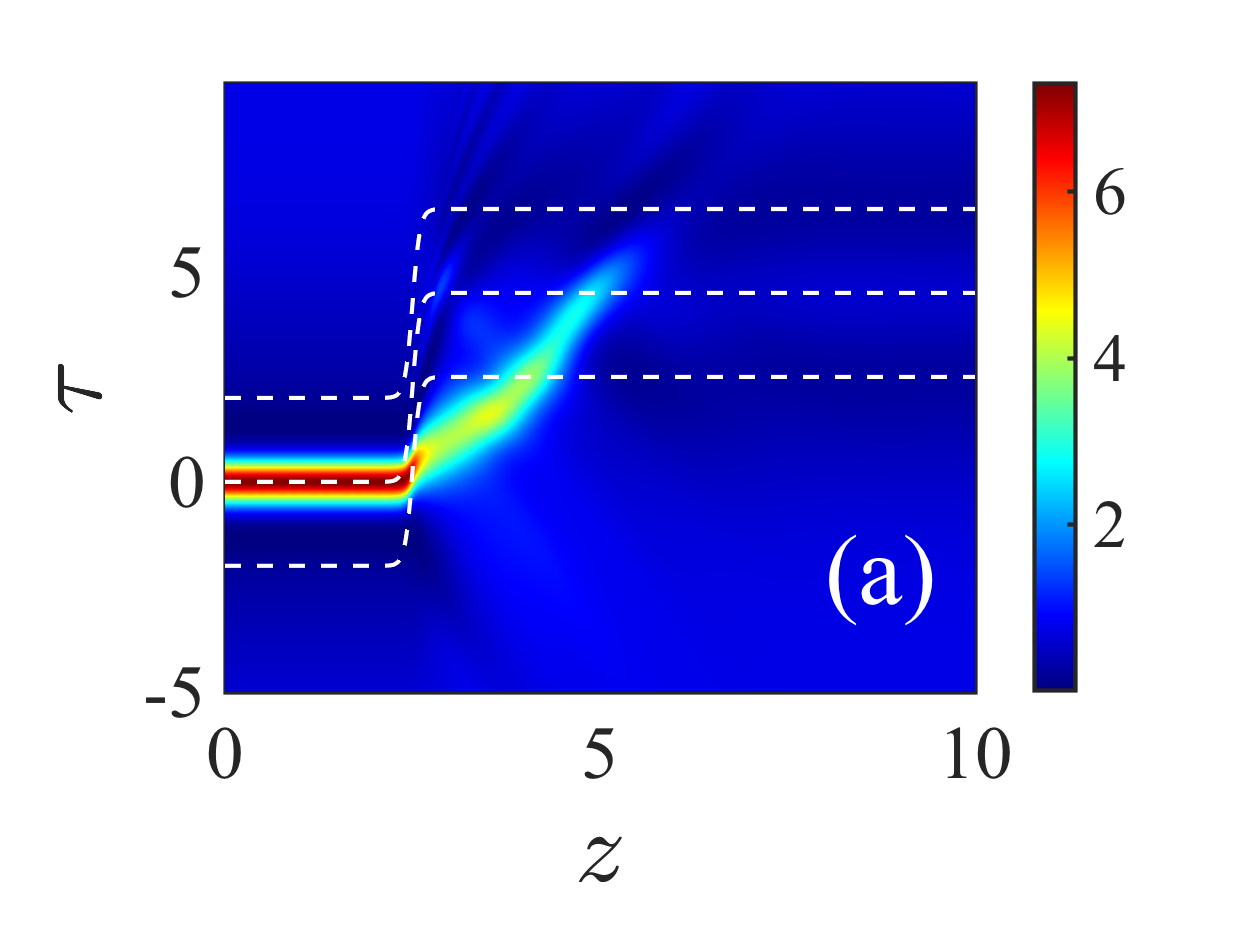
\includegraphics[width=\linewidth]{regularDensity5.eps} 
\caption{}
\end{subfigure}
\hspace{-1cm}
\begin{subfigure}{0.5\textwidth}
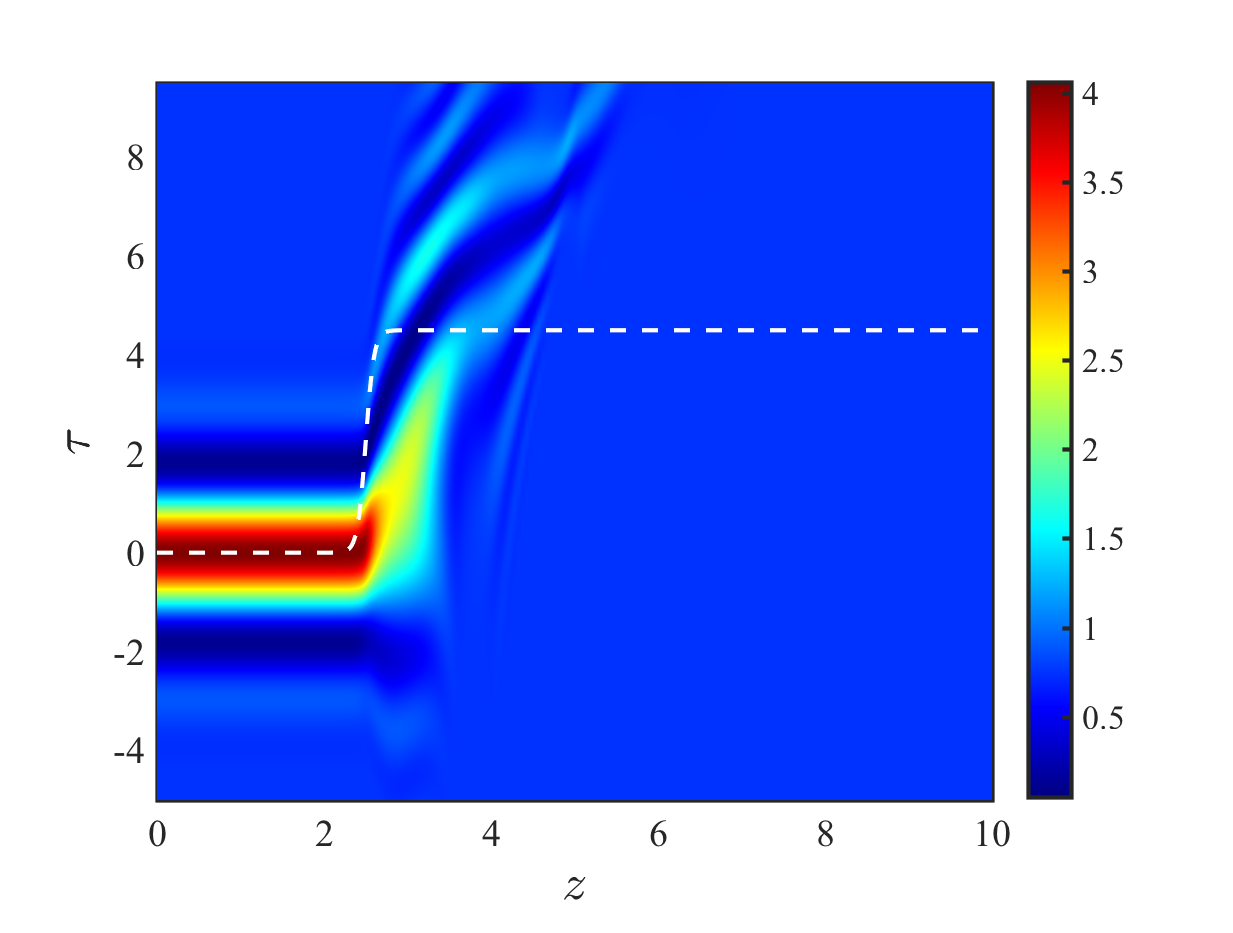
\includegraphics[width=\linewidth]{regularNCVADensity5.eps} 
\caption{}
\end{subfigure} }
\centerline{
\hspace{1cm}
\begin{subfigure}{\textwidth}
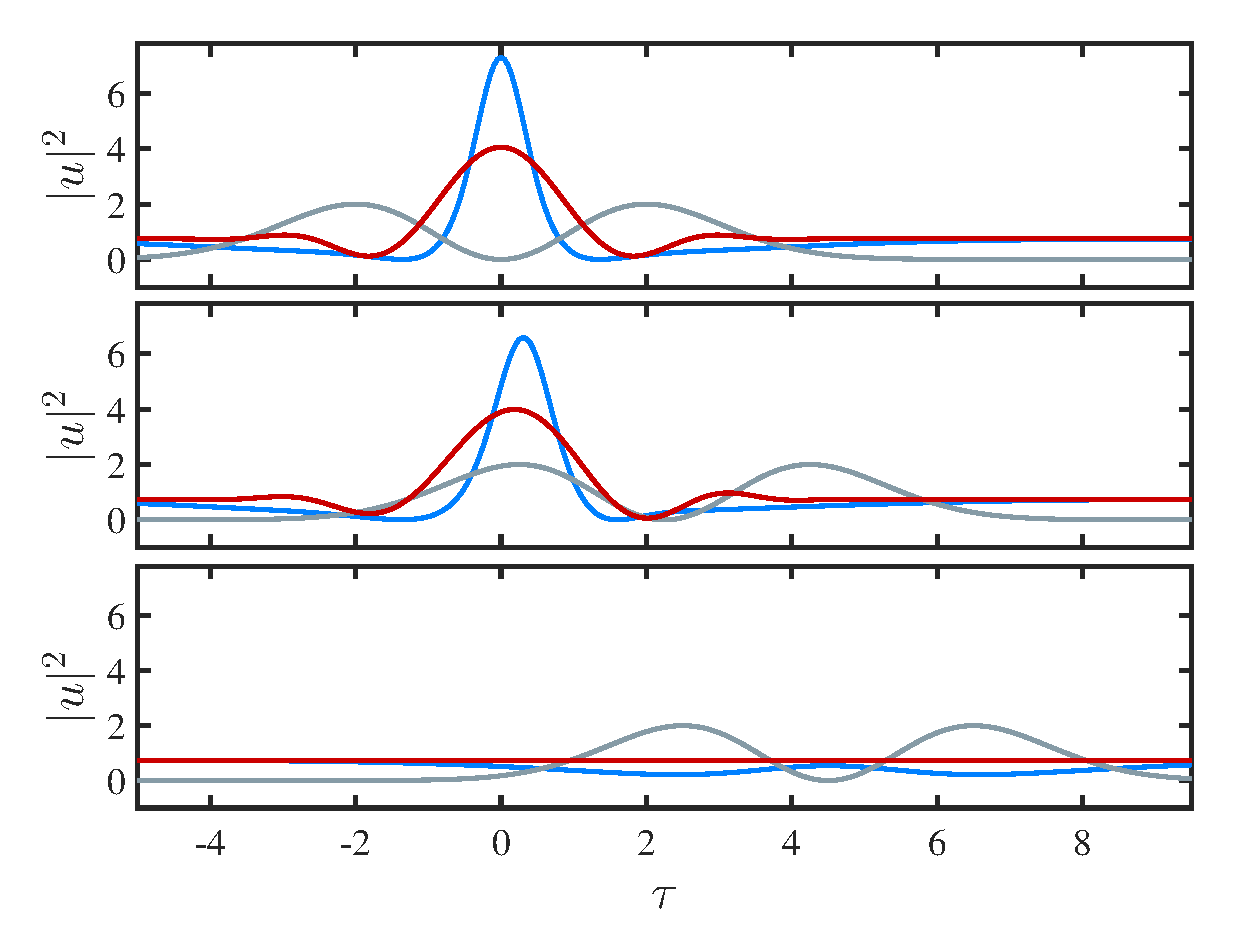
\includegraphics[width=0.9\linewidth]{regularTimeSeries5.eps} 
\caption{}
\end{subfigure}}
  \rule{35em}{0.5pt}
\caption[Dynamic Evolution of Natural Tweezer with no-CS]{Dynamic evolution as in Fig.~\ref{fig:Skinny1} but for $\tau_f = 4.5$ and $\beta = 10$.  Same layout as in Fig.~\ref{fig:Skinny1}.  In this sample, the NCVA and LL model solutions are both no-CS. 
}
\label{fig:Regular2}
\end{figure}

\begin{figure}[htb!]
\centering
\centerline{
\hspace{1cm}
\begin{subfigure}{0.5\textwidth}
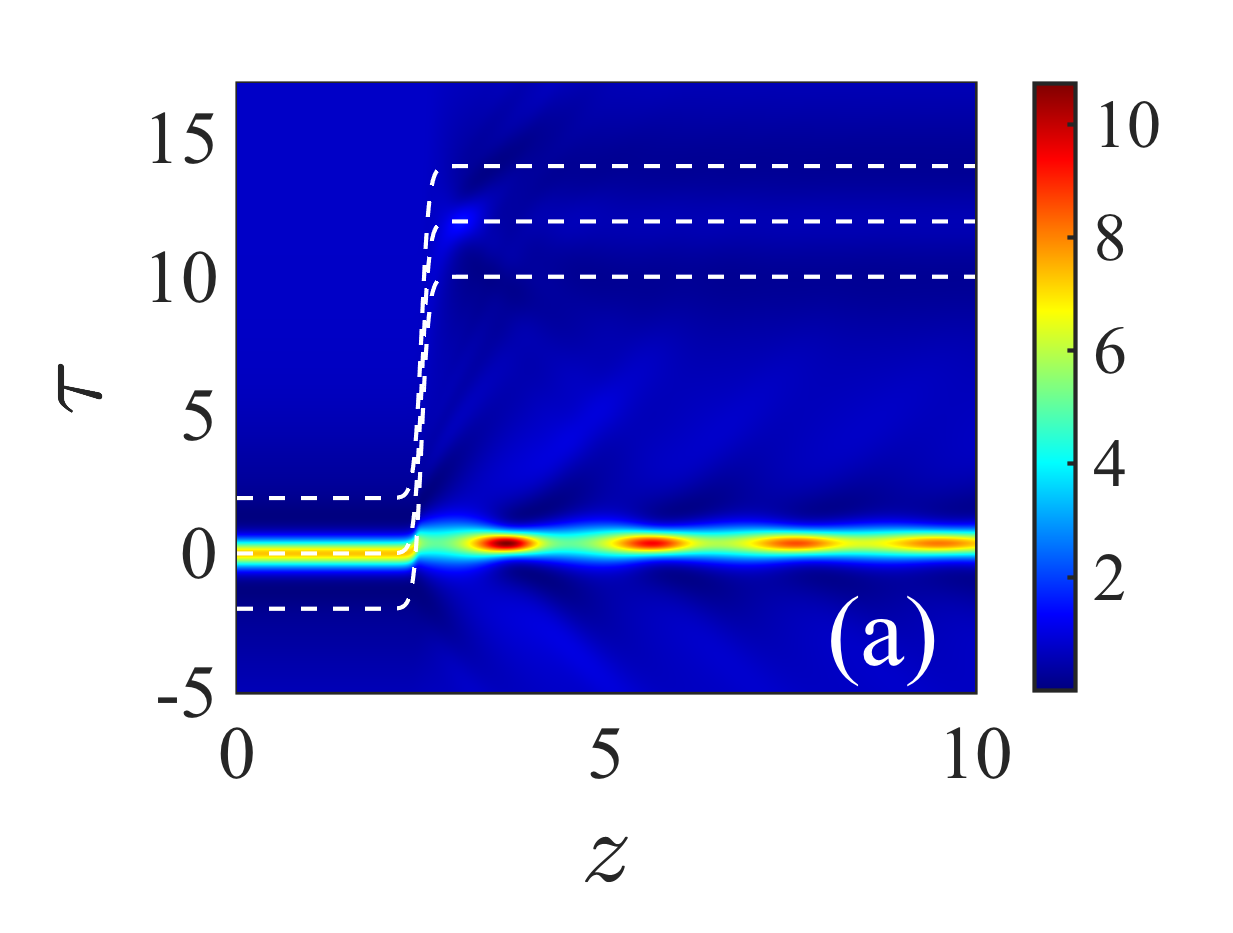
\includegraphics[width=\linewidth]{regularDensity3.eps} 
\caption{}
\end{subfigure}
\hspace{-1cm}
\begin{subfigure}{0.5\textwidth}
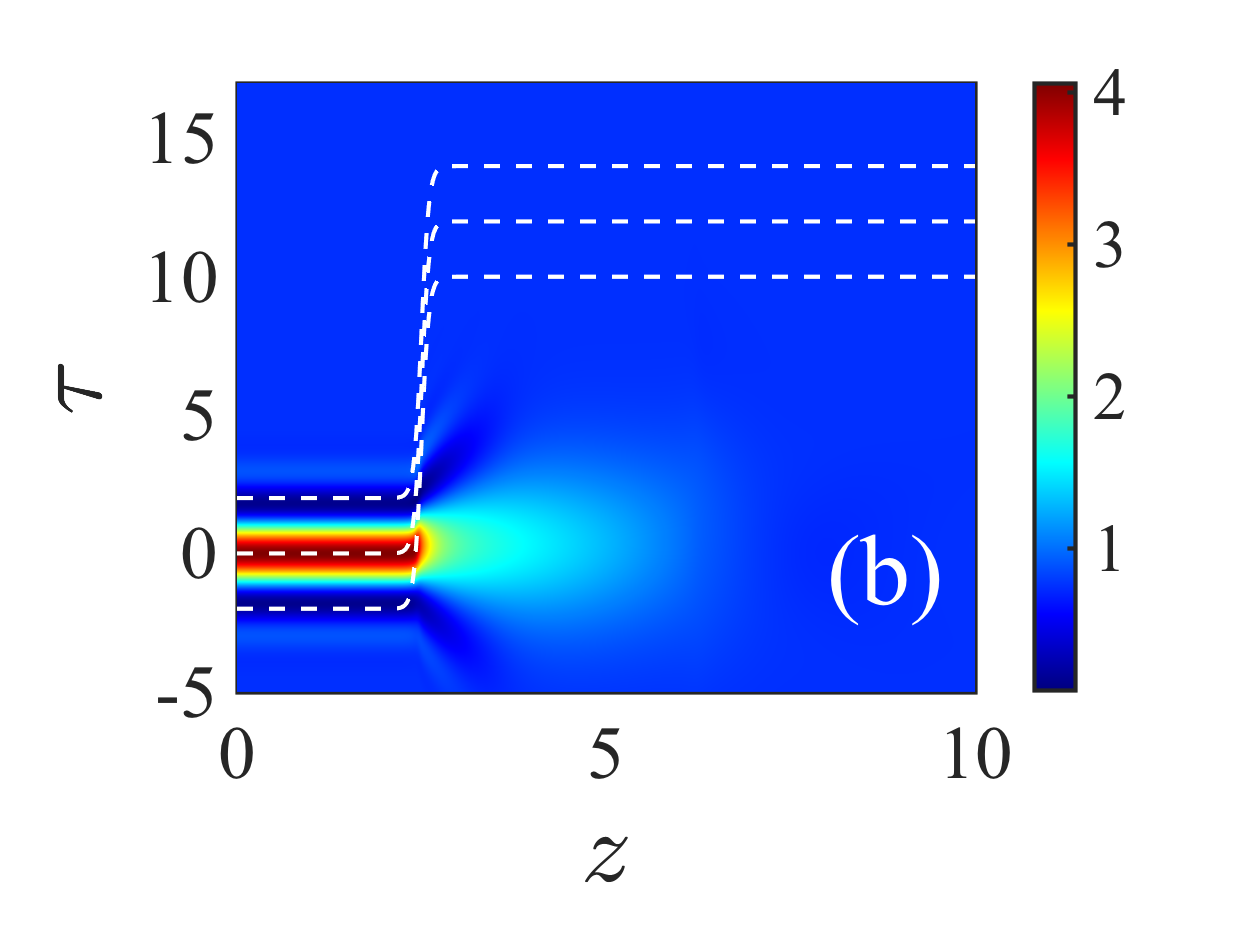
\includegraphics[width=\linewidth]{regularNCVADensity3.eps} 
\caption{}
\end{subfigure} }
\centerline{
\hspace{1cm}
\begin{subfigure}{\textwidth}
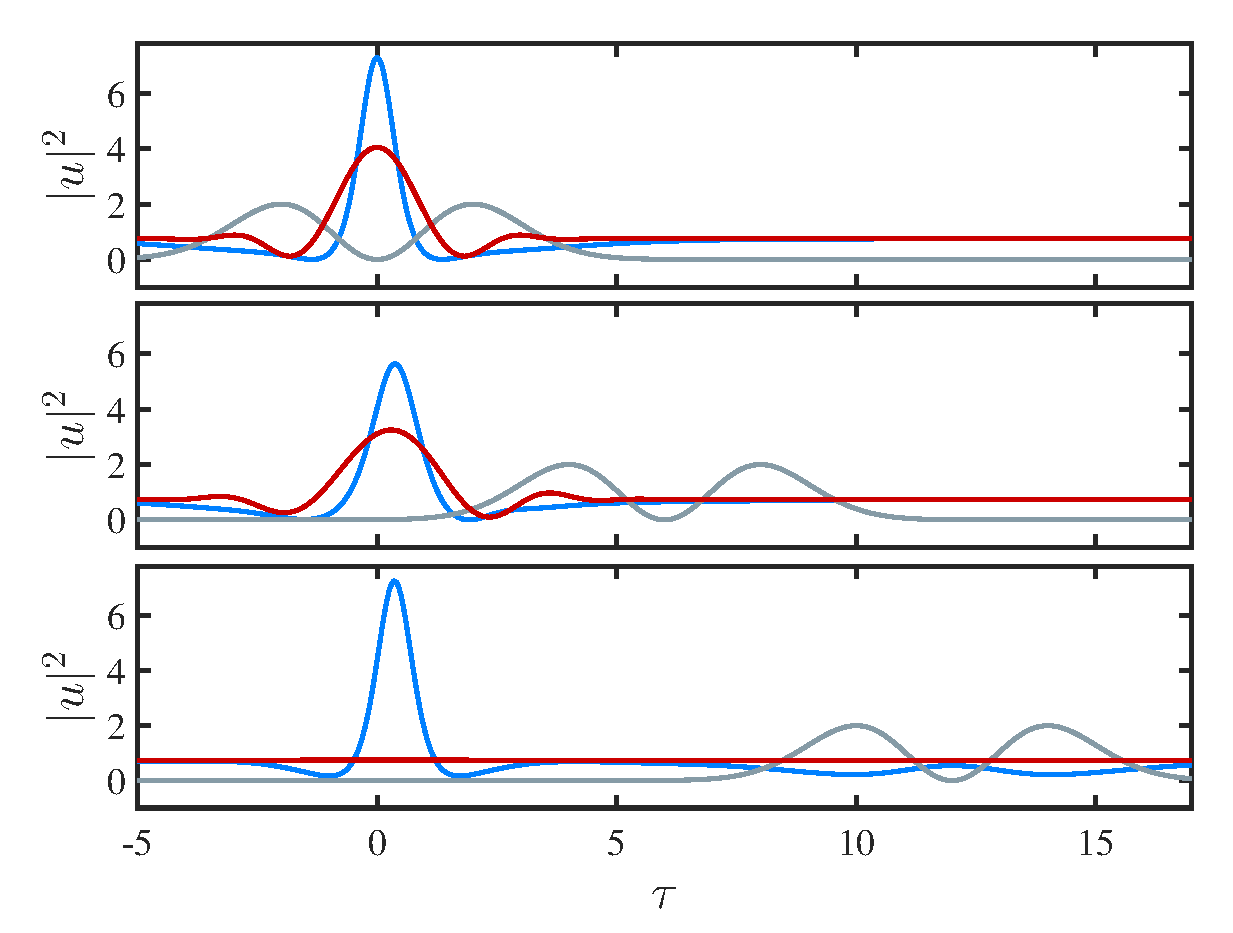
\includegraphics[width=0.9\linewidth]{regularTimeSeries3.eps} 
\caption{}
\end{subfigure}}  \rule{35em}{0.5pt}
\caption[Dynamic Evolution of Natural Tweezer with Non-Tweezed CS]{Dynamic evolution as in Fig.~\ref{fig:Skinny1} but for $\tau_f = 12$ and $\beta = 10$.  Same layout as in Fig.~\ref{fig:Skinny1}.  In this sample, the NCVA solution is a no-CS.  The CS of the LL model is stationary outside the natural width tweezer, which leaves the CS behind as the phase modulation is moved, referred to as a non-tweezed CS.
}
\label{fig:Regular3}
\end{figure}

\begin{figure}[htb!]
\centering
\centerline{
\hspace{1cm}
\begin{subfigure}{0.5\textwidth}
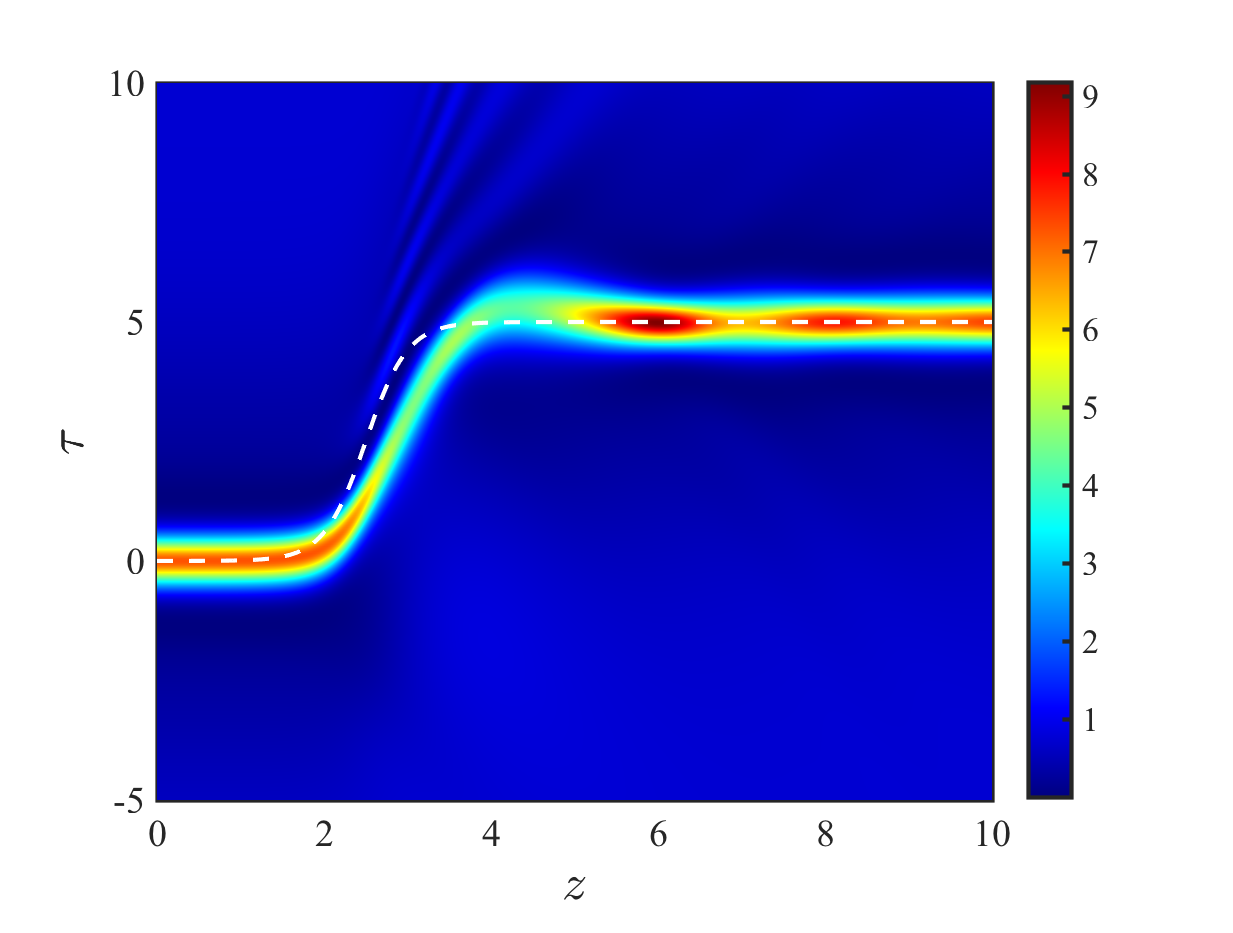
\includegraphics[width=\linewidth]{regularDensity4.eps} 
\caption{}
\end{subfigure}
\hspace{-1cm}
\begin{subfigure}{0.5\textwidth}
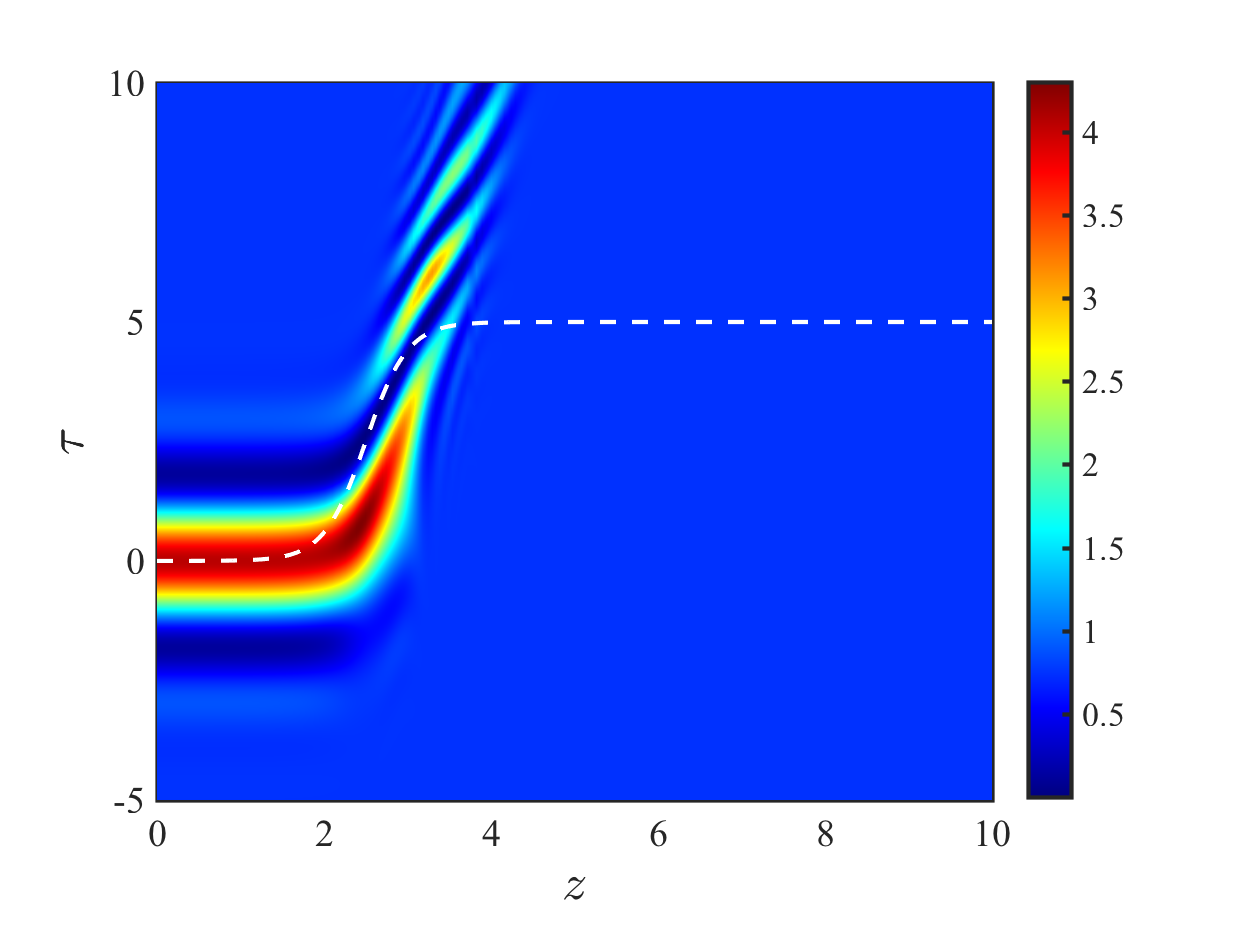
\includegraphics[width=\linewidth]{regularNCVADensity4.eps} 
\caption{}
\end{subfigure} }
\centerline{
\hspace{1cm}
\begin{subfigure}{\textwidth}
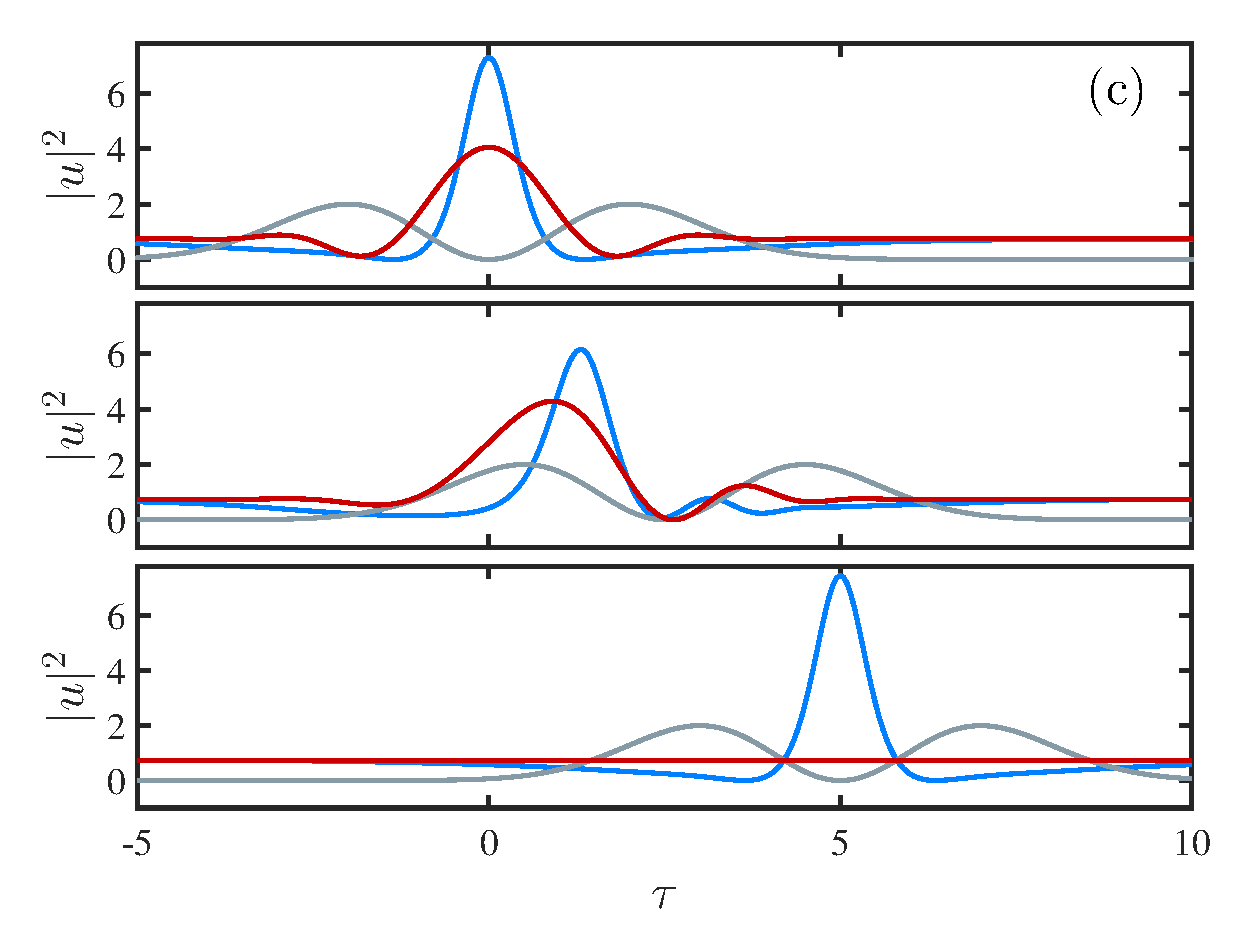
\includegraphics[width=0.9\linewidth]{regularTimeSeries4.eps} 
\caption{}
\end{subfigure}}
  \rule{35em}{0.5pt}
\caption[Dynamic Evolution of Natural Tweezer with LL Tweezed-CS and NCVA No-CS]{Dynamic evolution as in Fig.~\ref{fig:Skinny1} but for $\tau_f = 5$ and $\beta = 2$.  Same layout as in Fig.~\ref{fig:Skinny1}.  In this sample, the NCVA is a no-CS while the LL model is a tweezed-CS. 
}
\label{fig:Regular4}
\end{figure}

As a sample of the dynamic properties of tweezability, Fig.~\ref{fig:Regular1} is a tweezed CS (blue region Fig.~\ref{fig:RegularVsNCVA}) for both the full LL model and the NCVA.  Fig.~\ref{fig:Regular2} is the no-CS solution  (green region Fig.~\ref{fig:RegularVsNCVA}).  For the third sample, Fig.~\ref{fig:Regular3} the tweezer leaves the CS outside the effective potential in the full LL model while in the NCVA the solution is dissipative (red region Fig.~\ref{fig:RegularVsNCVA}), which can not be captured by the NCVA.  In contrast, Fig.~\ref{fig:Regular4} depicts the existence of a dissipative no-CS solution for both the full LL model and the NCVA (blue region Fig.~\ref{fig:RegularVsNCVA}).  As Figs.~\ref{fig:Regular1}(a) and (b) show, the initial state [see solid (blue) line LL model solution and solid (red) line NCVA solution in Fig.~\ref{fig:Regular1}(c) top panel] is manipulated by the natural width tweezer towards $\tau_f$ at speed $\beta$ [see solid (blue) line LL model solution  and solid (red) line NCVA solution in Fig.~\ref{fig:Regular1}(c) bottom panel], which we refer to as a tweezed CS in both the LL model and NCVA.  Figures~\ref{fig:Regular2}(a) and (b) show the initial state [see solid (blue) line LL model solution and solid (red) line NCVA solution in Fig.~\ref{fig:Regular2}(c) top panel] and as the CS is dragged the solution dissipates until there is no longer a CS, in agreement between the LL model and NCVA  [see solid (blue) line LL model solution and solid (red) line NCVA solution in Fig.~\ref{fig:Regular2}(c) bottom panel].   As Figs.~\ref{fig:Regular3}(a) and (b) show the initial state [see solid (blue) line LL model solution and solid (red) line NCVA solution in Fig.~\ref{fig:Regular3}(c) top panel] is left behind as the natural tweezer is displaced for the LL model and is completely lost in the case of the NCVA  [see solid (blue) line LL model solution  and solid (red) line NCVA solution in Fig.~\ref{fig:Regular3}(c) bottom panel].  \JMR{The NCVA and LL model thresholds do not always agree, as depicted in Fig.~\ref{fig:Regular4}.  As Figs.~\ref{fig:Regular4}(a) and (b) show, the initial state [see solid (blue) line LL model solution and solid (red) line NCVA solution in Fig.~\ref{fig:Regular4}(c) top panel] is manipulated by the natural width tweezer towards $\tau_f$ at speed $\beta$ [see solid (blue) line LL model solution  and solid (red) line NCVA solution in Fig.~\ref{fig:Regular4}(c) bottom panel], which we refer to as a tweezed CS for the LL model and no-CS for the NCVA.}


\setstretch{1.3}
\subsection[Tweezer with Wide Width]{Tweezer with Wide Width} \label{section:Fat}
\setstretch{2}

\vspace{-0.5cm}
In the third case study, we are interested in a tweezer with a wide width $\sigma_\phi = 3$ and height $h_\phi = 6.9949$ by Eq.~(\ref{height}).  For the full LL Eq.~(\ref{eq:LLETweeze}), the steady state CS is found centered at $\tau_0 = 0$ using a Newton-Krylov solver and the power-balance constraint Eq.~(\ref{LLConstraint}) which selects a particular detuning parameter $\Delta = 3.0859$ for the system.  The setup is the same as in the other examples.

\begin{figure}[htb!]
\centering
\centerline{
\hspace*{0cm}
\begin{subfigure}{0.5\textwidth}
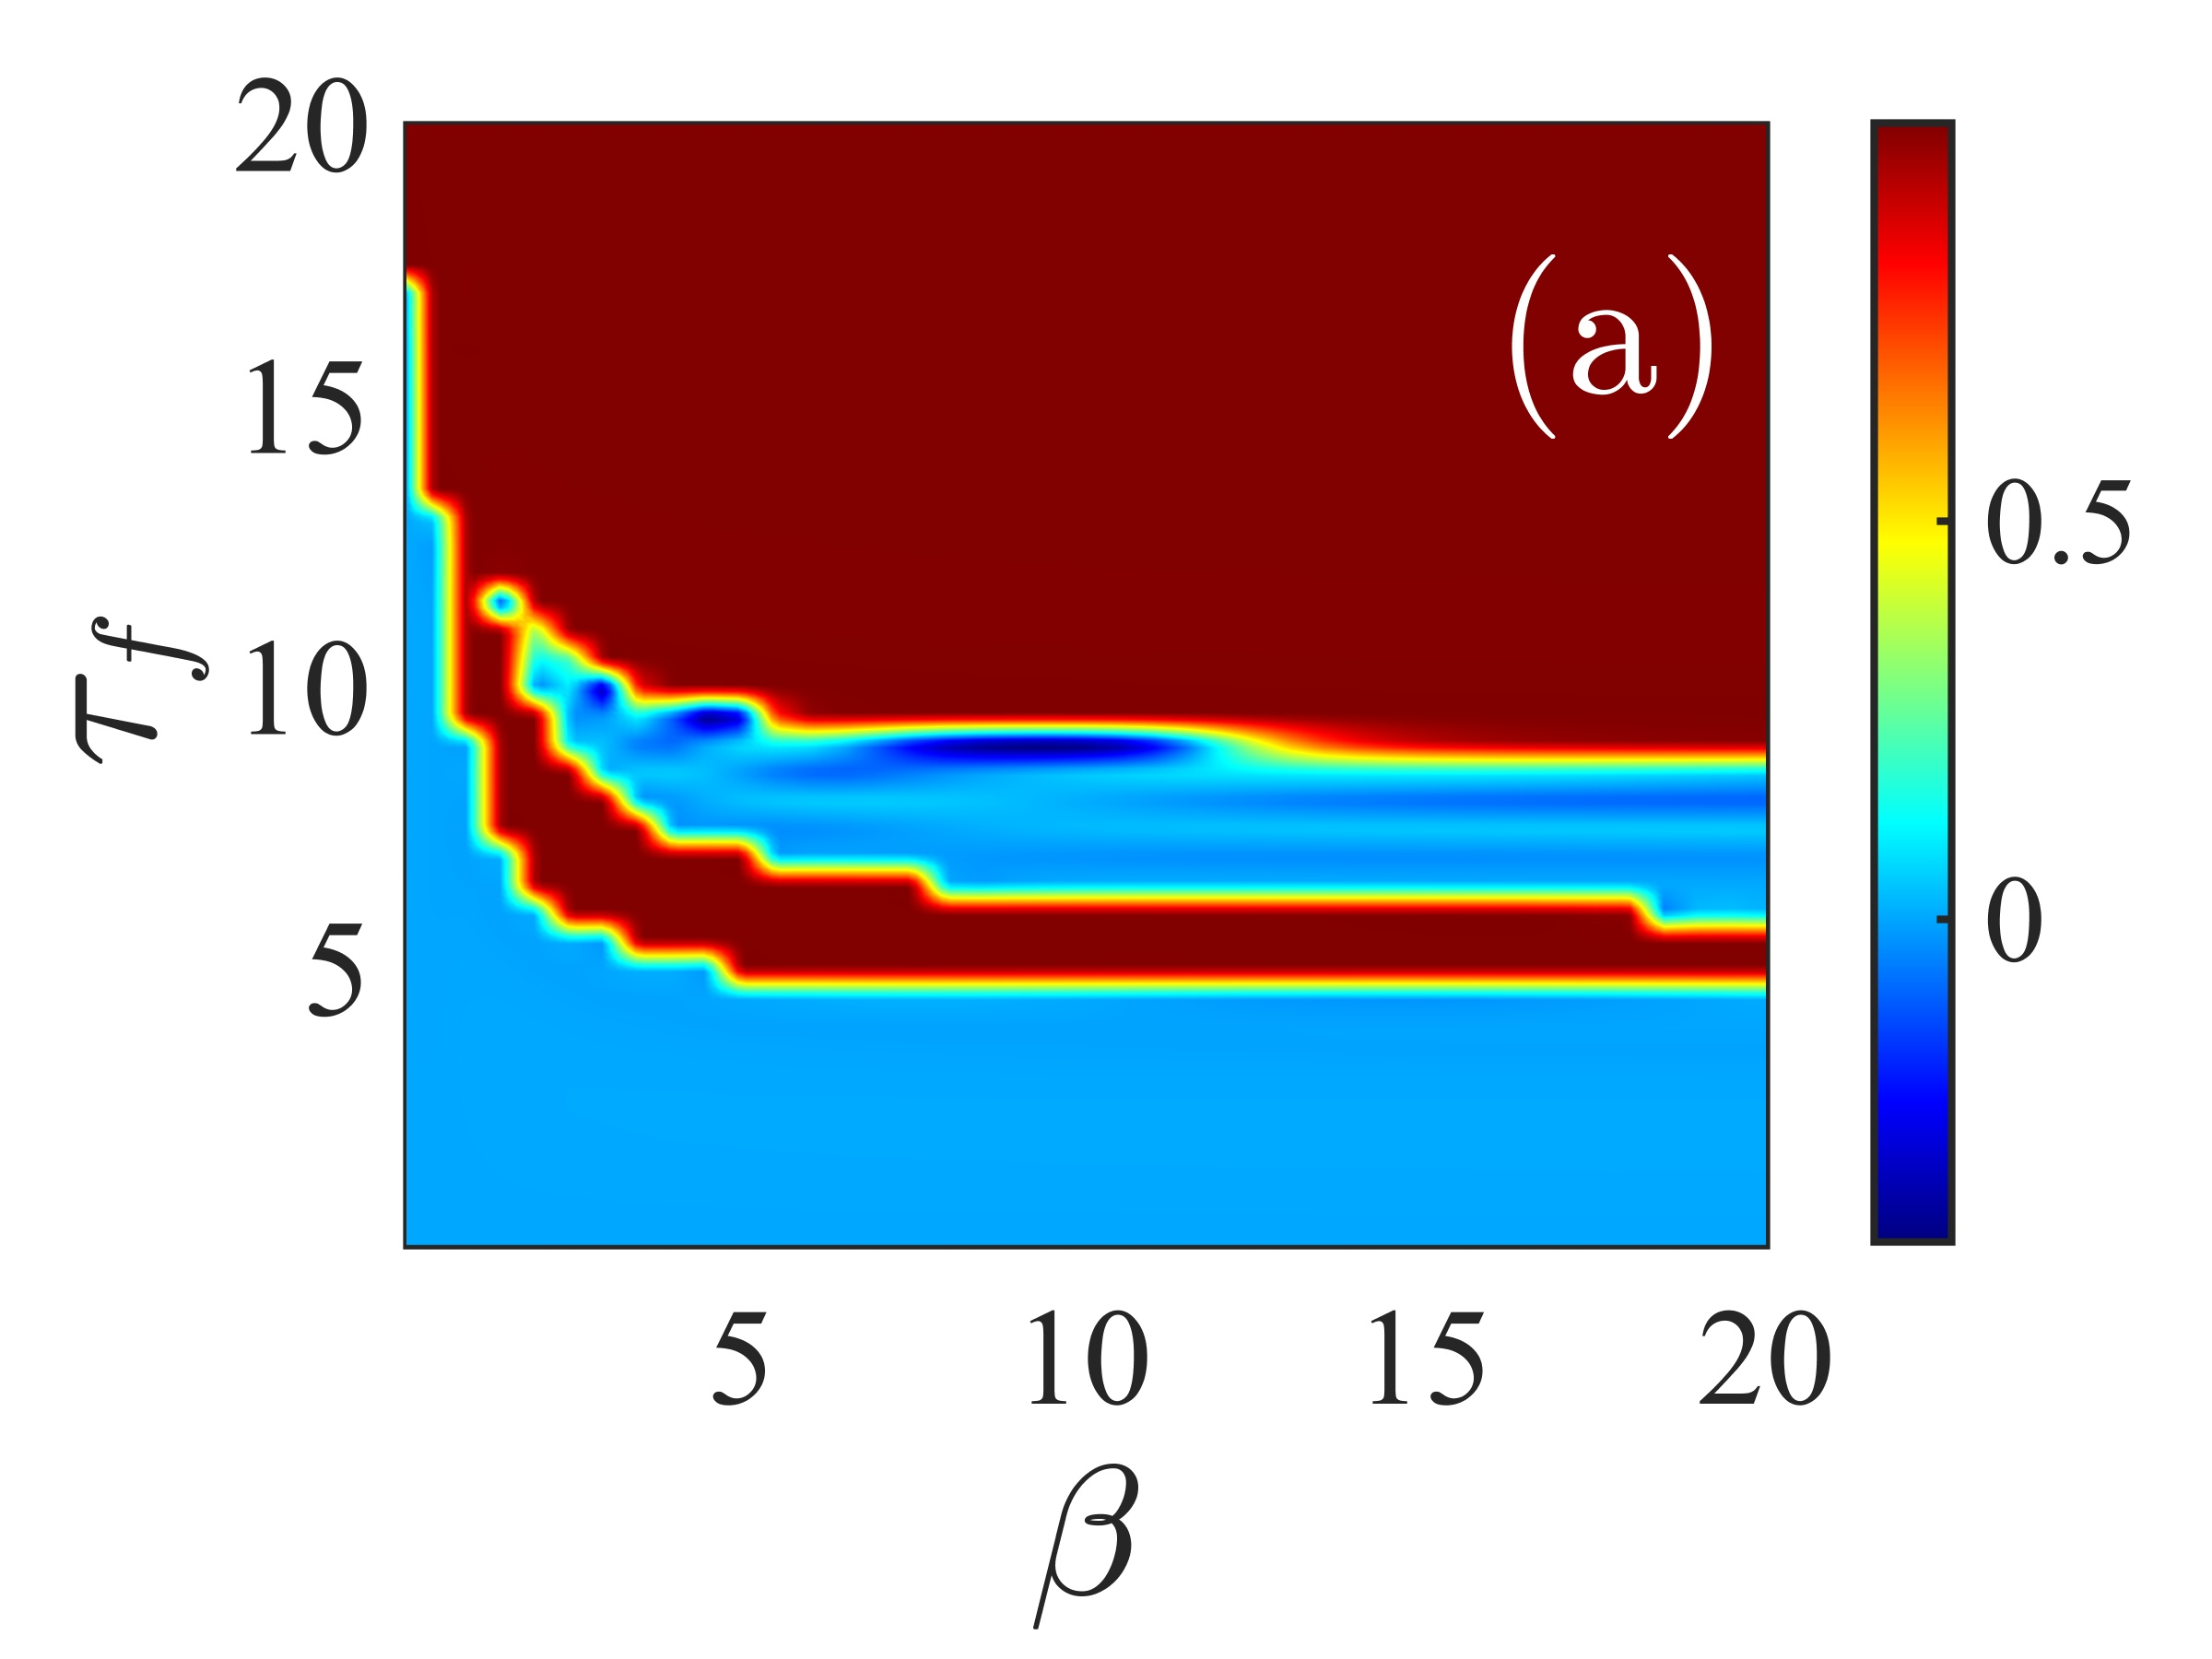
\includegraphics[width=\linewidth]{FatQIn.jpg}
\caption{} 
\end{subfigure}
%\hspace*{\fill}
\hspace*{-0.5cm}
\begin{subfigure}{0.5\textwidth}
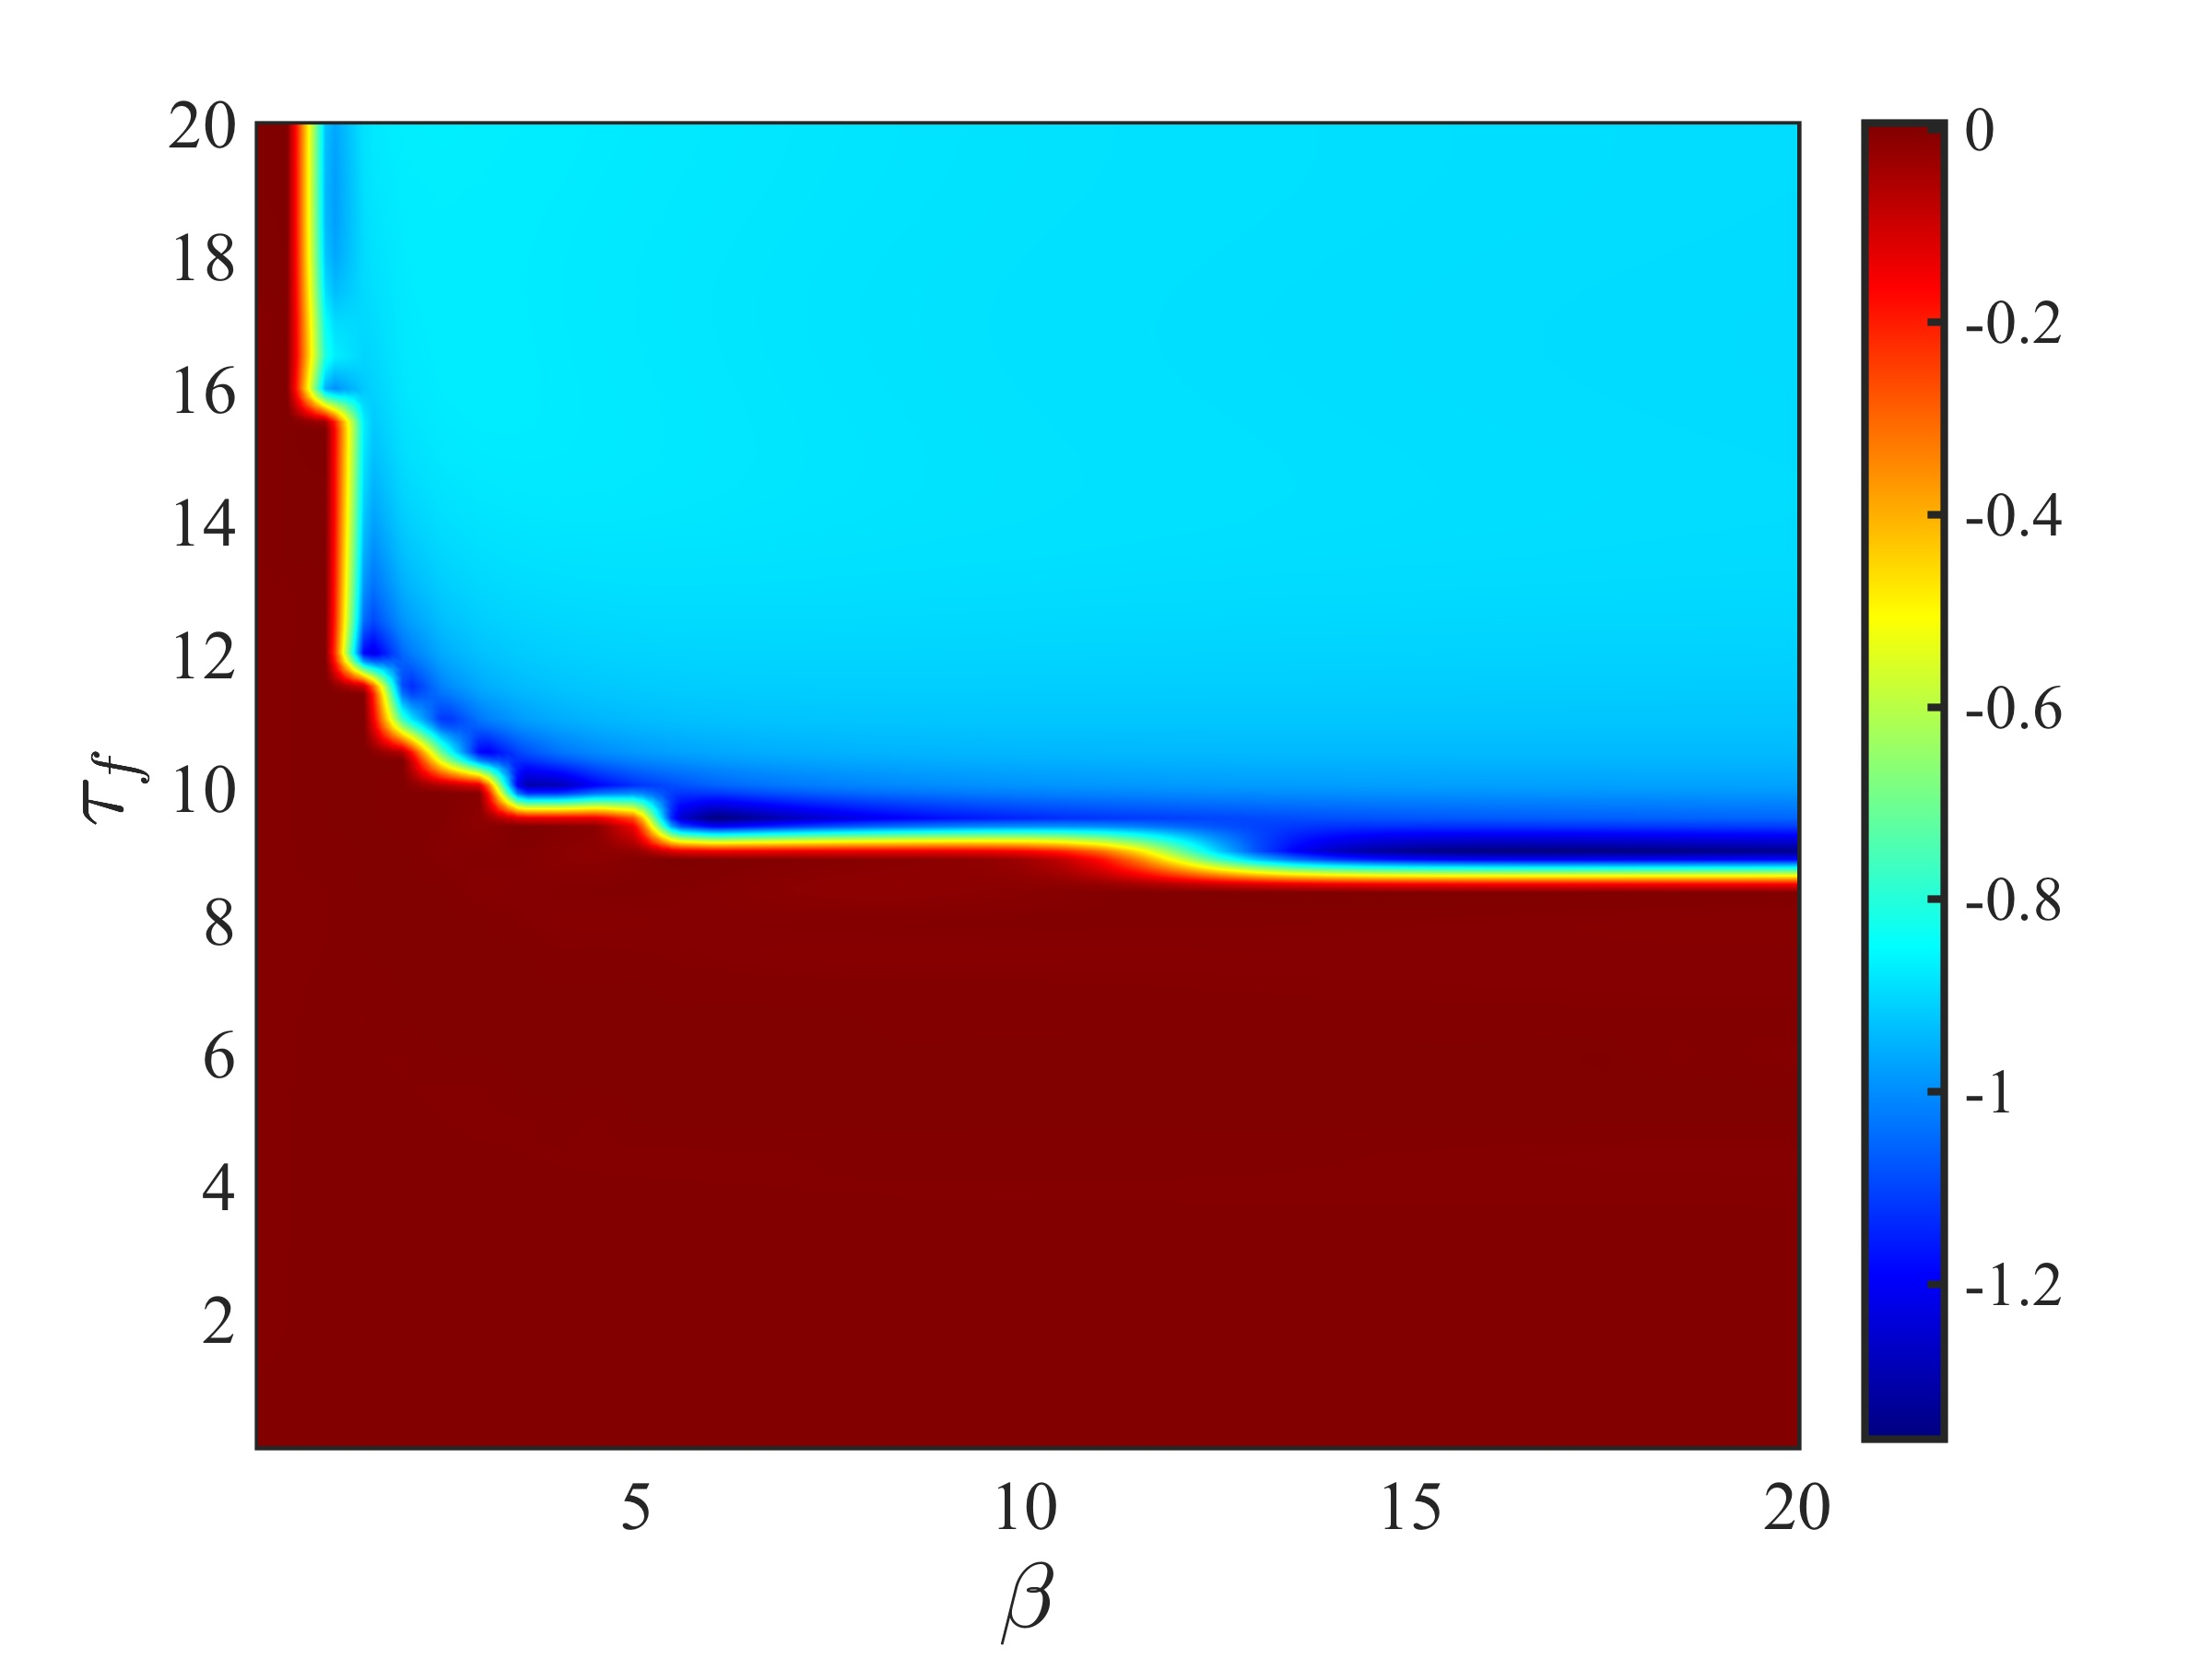
\includegraphics[width=\linewidth]{FatQOut.jpg} 
\caption{} 
\end{subfigure} }
\centerline{
\begin{subfigure}{\textwidth}
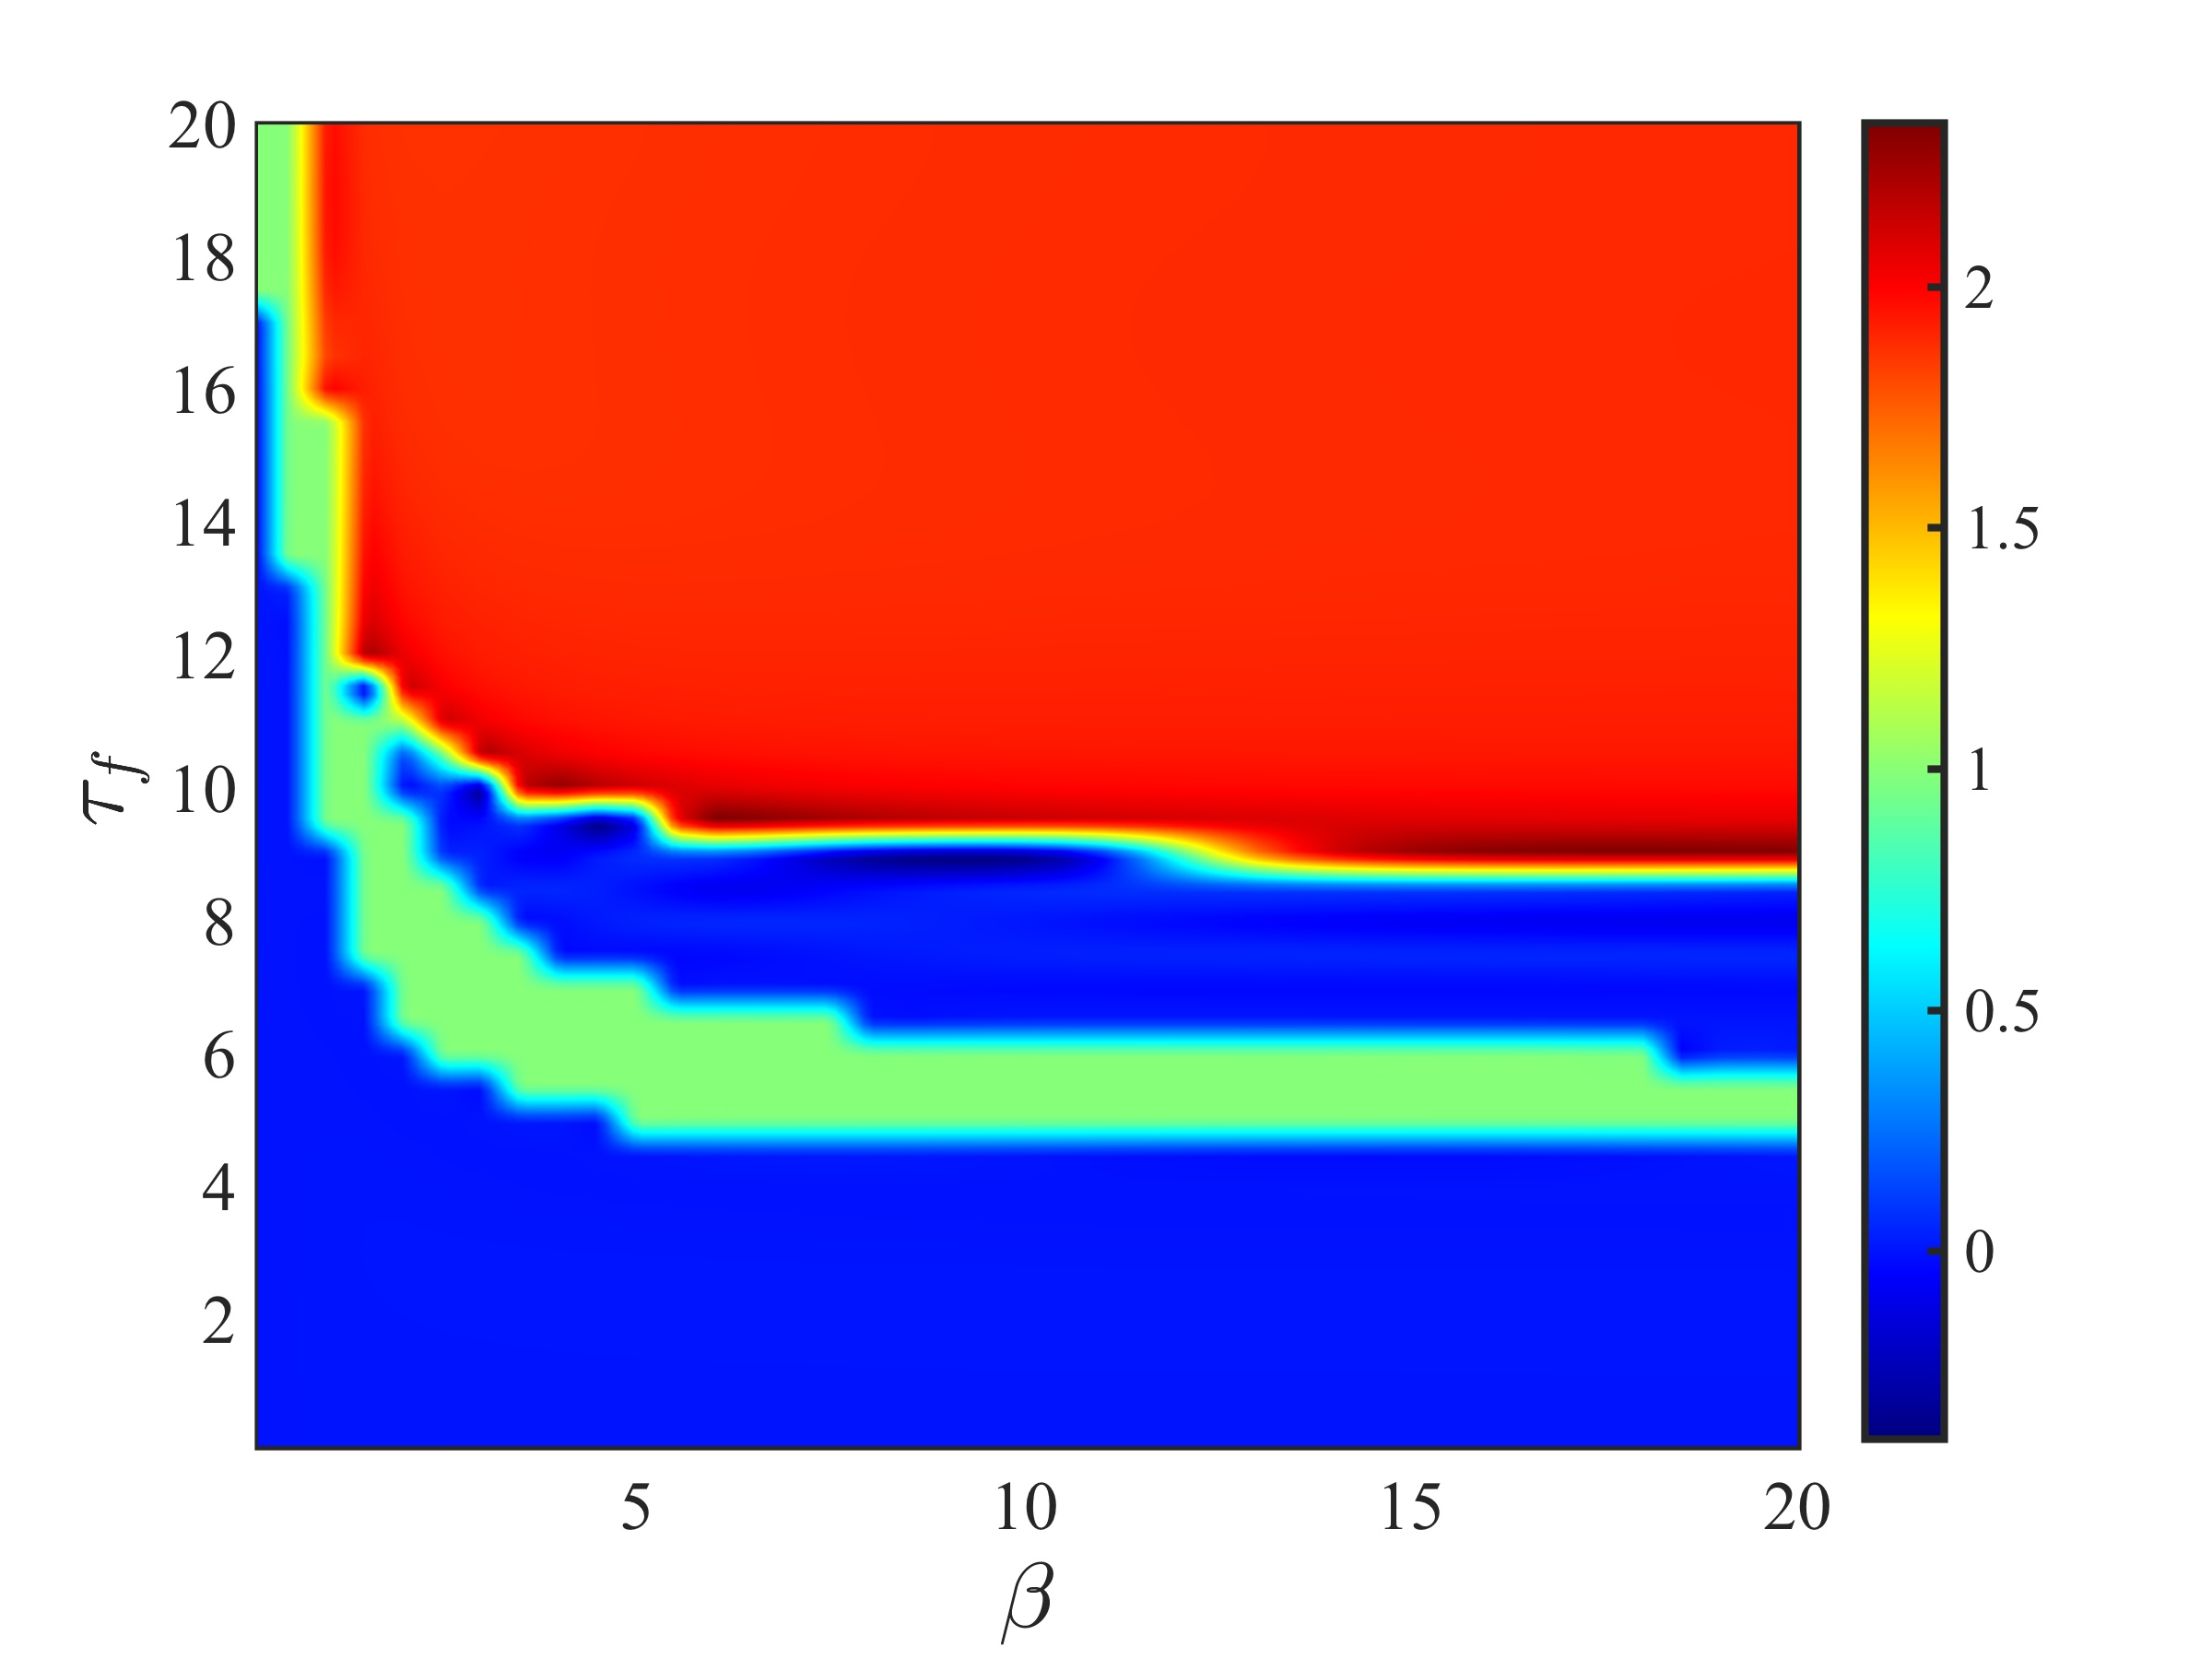
\includegraphics[width=0.9\linewidth]{FatQDiff.jpg} 
\caption{} 
\end{subfigure} }
  \rule{35em}{0.5pt}
\caption[Power Ratios Inside and Outside Tweezer with Wide Width]{Power ratios as in Fig.~\ref{fig:SkinnyQ} but for a natural tweezer with width $\sigma_\phi = 2$ and height $h_\phi = 6.9949$.  The detuning for the system is $\Delta =  3.0859$.   Same layout as in Fig.~\ref{fig:SkinnyQ}.  The difference power ratio (c) defines the thresholds for a tweezed CS for all blue regions, a no-CS for all green regions, and non-tweezed for all orange regions.  
}
\label{fig:FatQ}
\end{figure}

\begin{figure}[htb!]
\centerline{
\begin{subfigure}{0.5\textwidth}
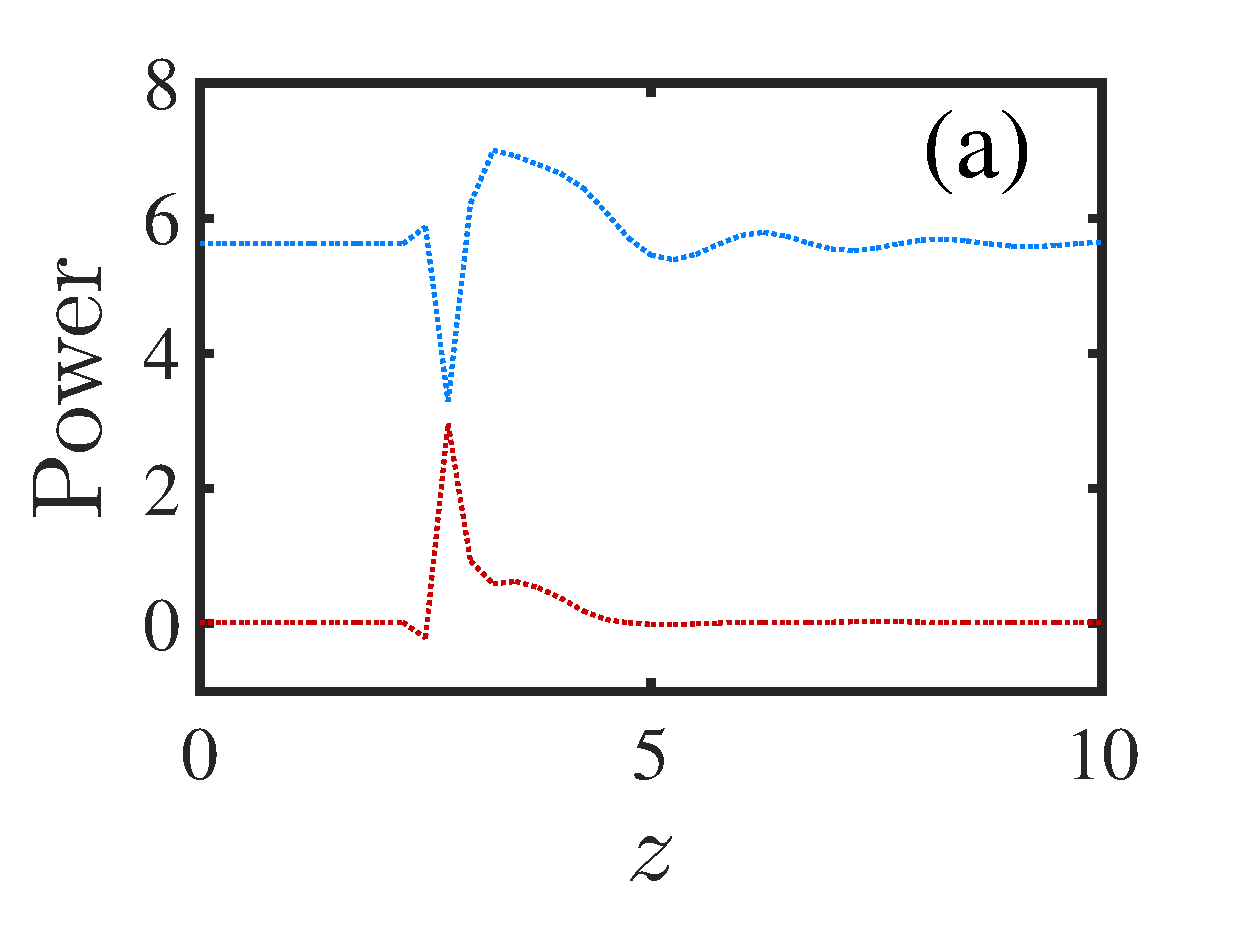
\includegraphics[width=\linewidth]{fatTimeMass1.eps} 
\caption{}
\end{subfigure}
\begin{subfigure}{0.5\textwidth}
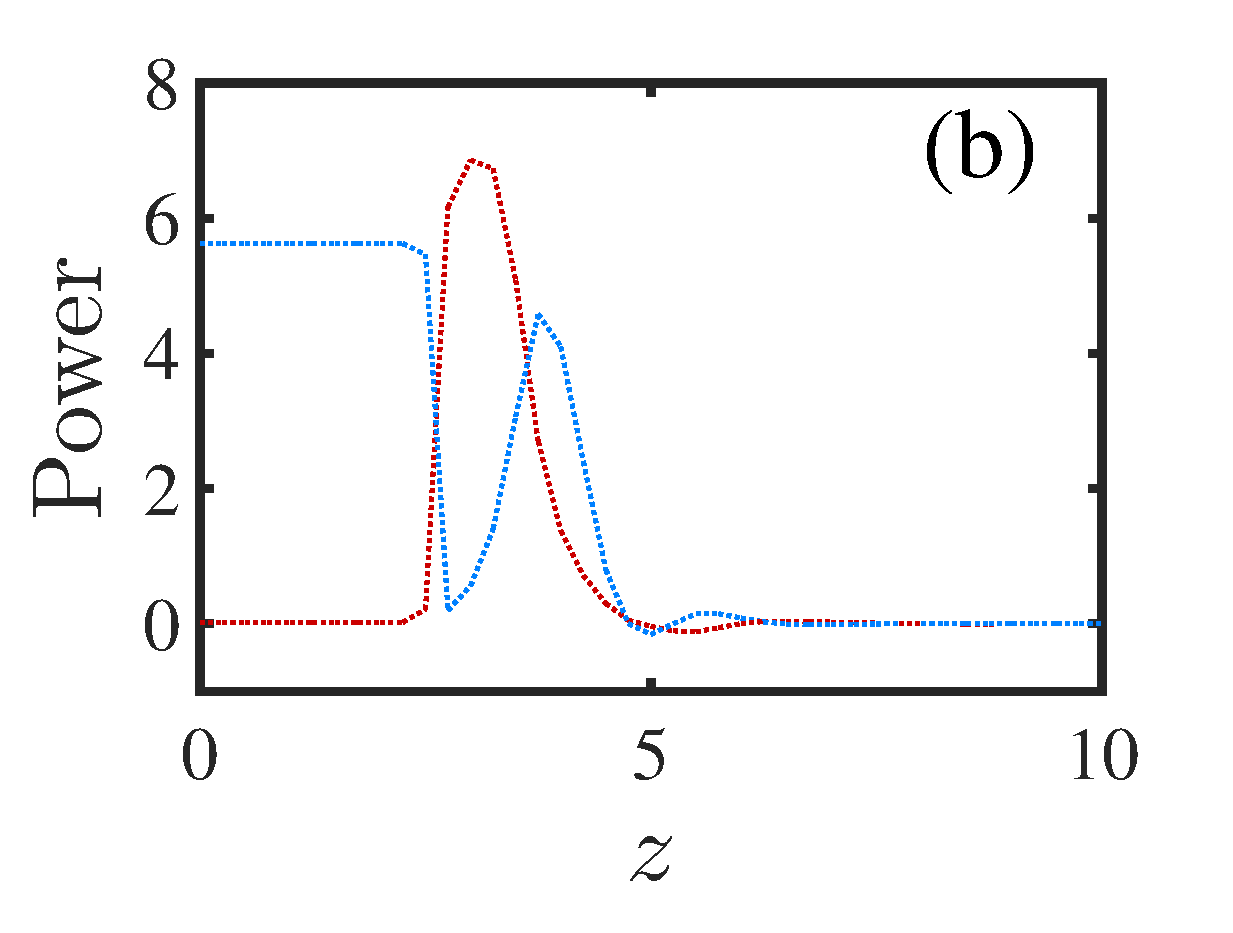
\includegraphics[width=\linewidth]{fatTimeMass2.eps} 
\caption{}
\end{subfigure} }
\centerline{\begin{subfigure}{0.5\textwidth}
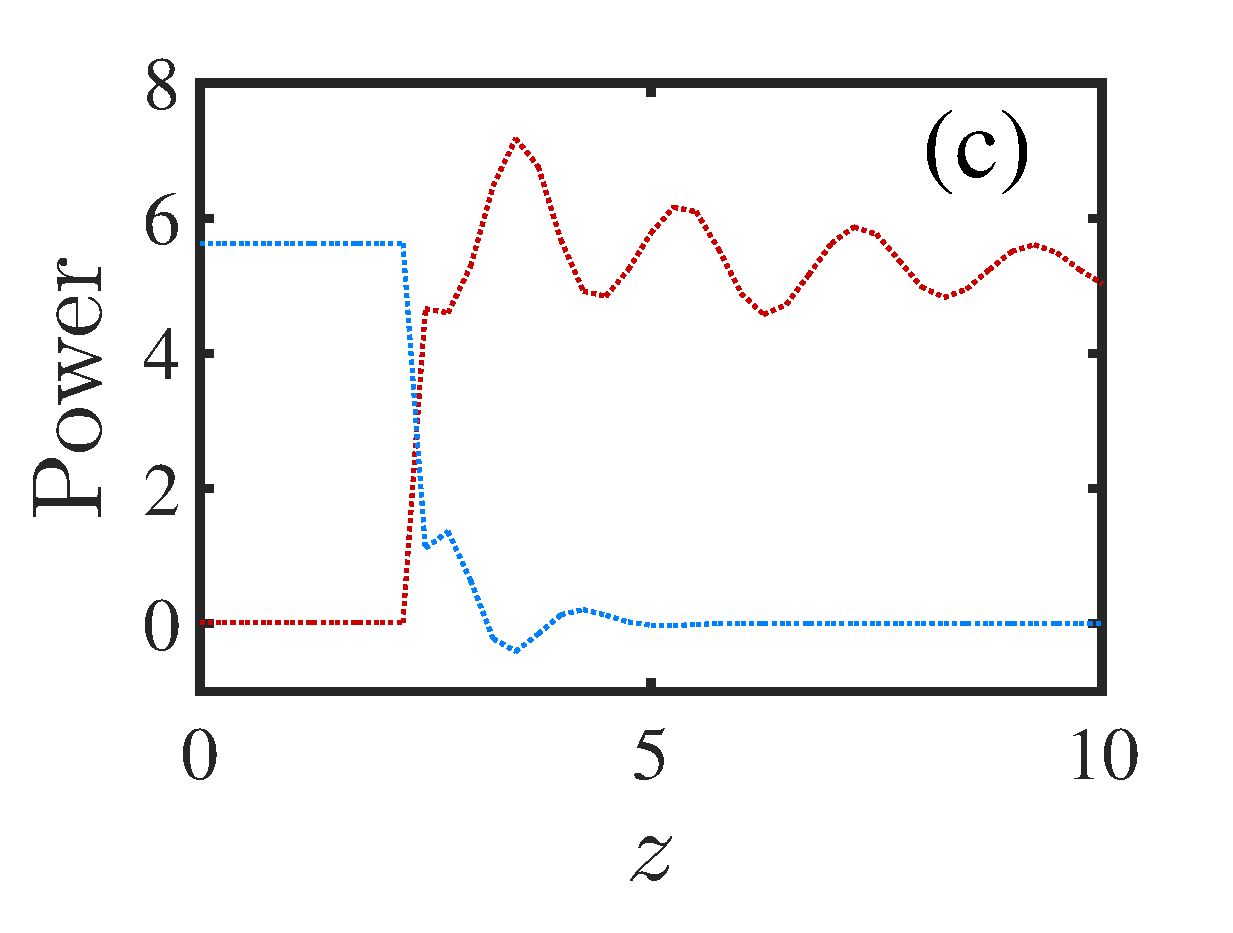
\includegraphics[width=\linewidth]{fatTimeMass3.eps} 
\caption{}
\end{subfigure} 
\begin{subfigure}{0.5\textwidth}
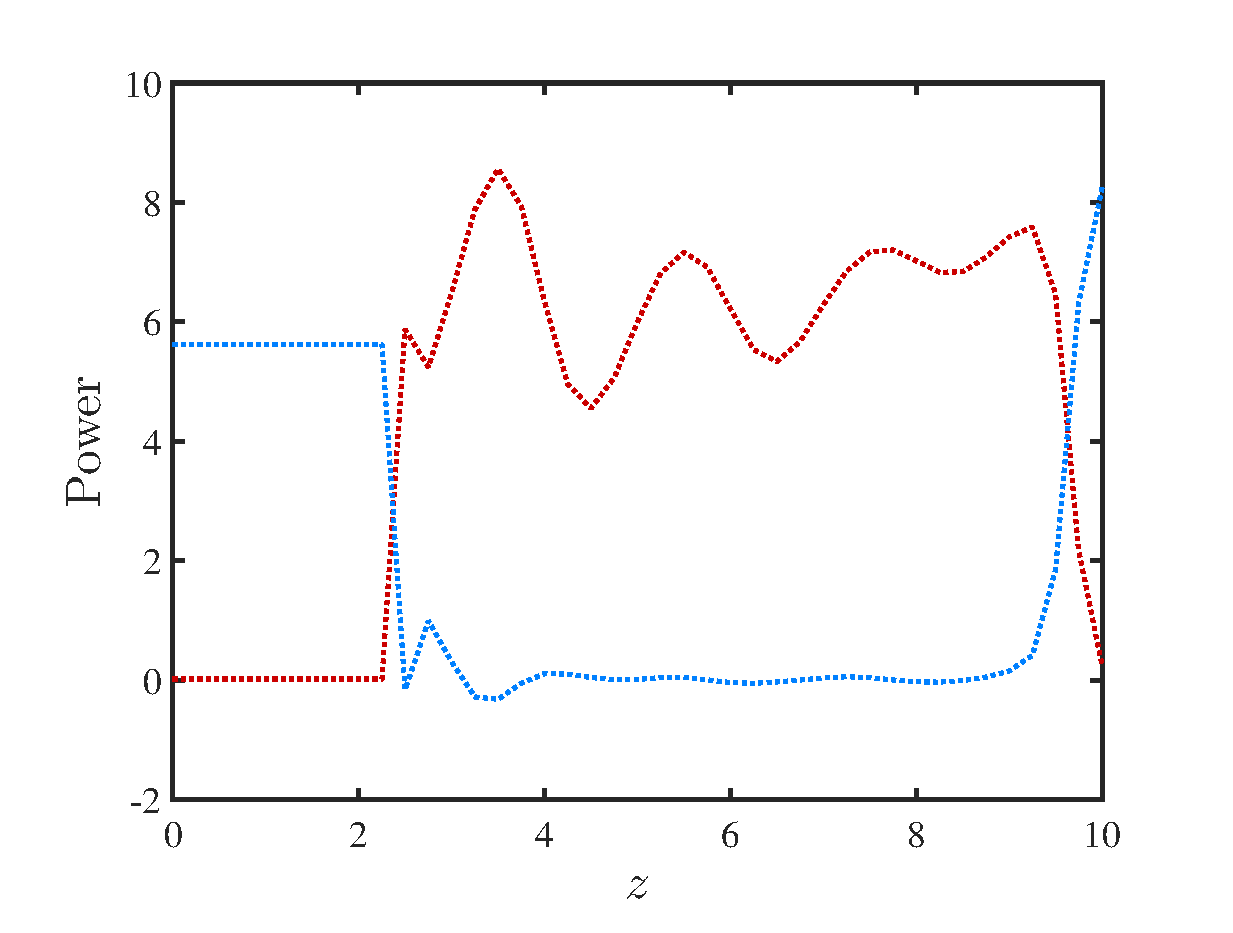
\includegraphics[width=\linewidth]{fatTimeMass5.eps}
\caption{}
\end{subfigure} } 
 \rule{35em}{0.5pt}
\caption[Tweezer with Wide Width Power Comparison]{Comparison of the powers as in Fig.~\ref{fig:SkinnyComp} but for a wide tweezer.  Same layout as Fig.~\ref{fig:SkinnyComp}, but for parameters (a) $\tau_f = 4$ and $\beta=10$, (b) $\tau_f = 5.5$ and $\beta=10$, (c) $\tau_f = 18$ and $\beta=10$ and (d) $\tau_f = 9$ and $\beta=10$.  The left top panel (a) has no change in power inside or outside the tweezer which describes a tweezed CS, while right top panel (b) shows fluctuations caused by an uneven tweezing.  The left bottom panel (c) is an example of the tweezer moving too quickly and leaving the CS outside the tweezer.  The right bottom panel (d) is ``artificial'' tweezing, in which the trap initially loses the CS but but $z_f$ the CS catches up the tweezer.
}
\label{fig:FatComp}
\end{figure}

\begin{figure}[htb!]
\centering
\centerline{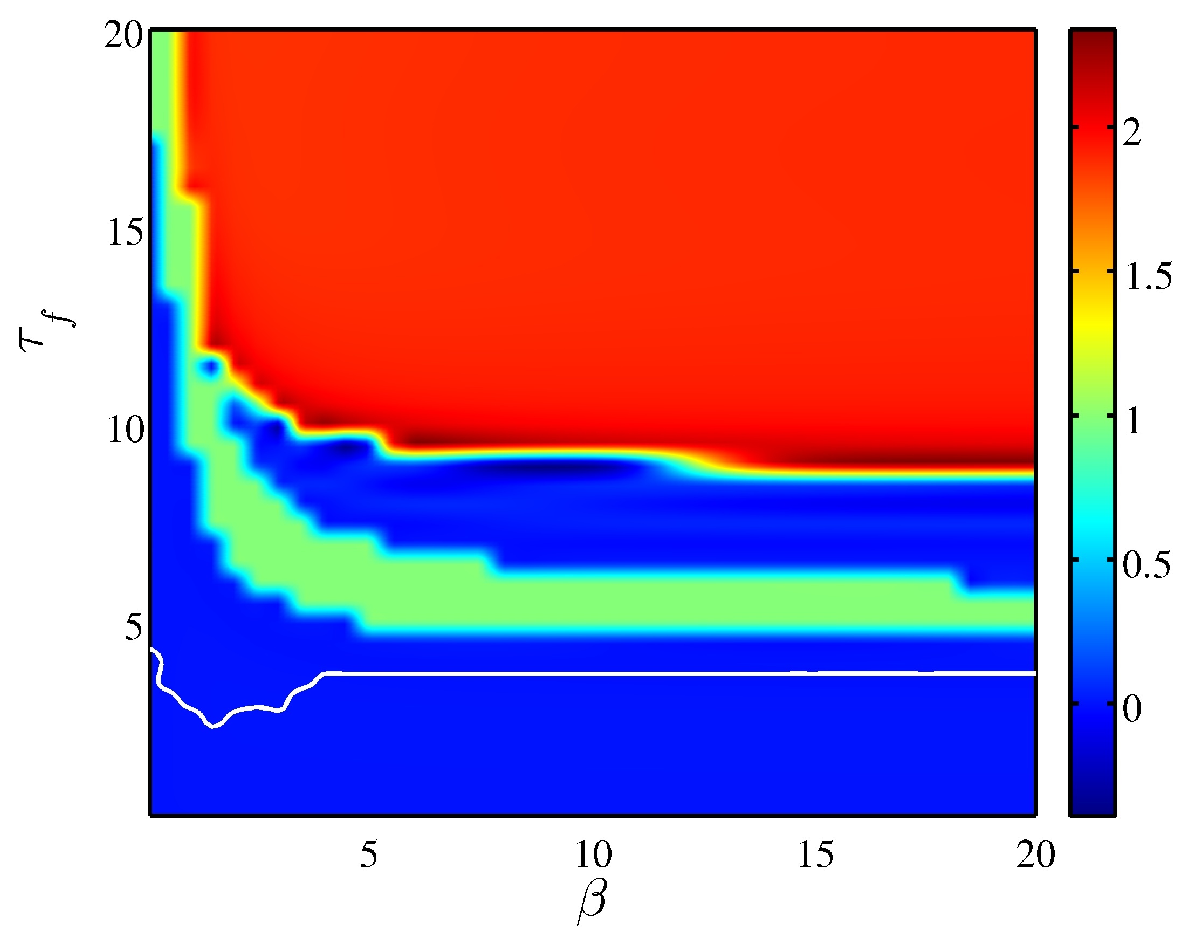
\includegraphics[width=0.9\textwidth]{FatPDEvODE_rcg_t.eps}}
  \rule{35em}{0.5pt}
\caption[Comparison of Power Ratio Inside Wide Tweezer for LL Model and NCVA]{Comparison of difference in power ratios between the NCVA and LL model as in Fig.~\ref{fig:SkinnyVsNCVA} but for a wide tweezer.  Same layout as Fig.~\ref{fig:SkinnyVsNCVA}.  The NCVA distinguishes a threshold between tweezed and no-CS solution at $\tau_f\approx 4$.  The LL model displays tweezed CSs in the blue region (under the green region), no-CSs in the green region, and a non-tweezed CSs in red region.  The blue region between the green and red regions is ``artificial'' tweezing, in which the trap initially loses the CS but at $z_f$ the CS catches up and is re-trapped by the tweezer.
}
\label{fig:fatVsNCVA}
\end{figure}

Figure~\ref{fig:FatQ} depicts the density of the power ratios as well as the difference Fig.~\ref{fig:FatQ} with the same layout as Fig.~\ref{fig:SkinnyQ} but for the wide tweezer.  The wide tweezer is defined by three fundamental evolutions: a tweezed CS for all $\beta$ when $0<\tau_f < 5$, no-CS for most $\beta$ when $5<\tau_f <14$, and a non-tweezed CS for all $\beta$ when $\tau_f > 14$.  The threshold for the existence of the tweezed CS with a wide tweezer is only marginally larger than that found for a natural width tweezer.

In order to better explain the power ratio, we examine four examples of the power inside $P_{\rm I}$ Eq.~(\ref{Pin}) and outside $P_{\rm O}$ Eq.~(\ref{Pout}) for $\beta = 10$ with $\tau_f = 4$, 5.5, 9, and 18 in Fig.~\ref{fig:FatComp}.  In Fig.~\ref{fig:FatComp} the red lines are $P_{\rm I}$ and the blue lines are $P_{\rm O}$.  Panel (a), $\beta = 10$ at $\tau_f = 4$, depicts a case that has no change in power inside or outside the tweezer which describes a tweezed CS, while panel (b), $\beta = 5.5$ at $\tau_f = 10$, shows complete loss of power inside which describes a no-CS.  Panel (c), $\beta = 10$ at $\tau_f = 18$, depicts an example of the non-tweezed CS.  Panel (d), for $\beta = 10$ and $\tau_f = 9$, depicts an ``artificially'' tweezed CS defined by the complete loss of the CS from the trap, but rather than a stationary CS left outside the trap (as is the case in non-tweezed CS), the CS is imparted with enough energy to continue moving in the direction of the tweezer.  By the final time $z_f$, the CS catches up and it is re-trapped by the tweezer and results in $P_{\rm I} \approx 1$ despite this case not being a true tweezed CS. 

Using the same layout as Fig.~\ref{fig:SkinnyVsNCVA}, Fig.~\ref{fig:fatVsNCVA} compares the difference in quotient ratios between the NCVA and the full LL model.  The NCVA threshold between the tweezed CS and no-CS is approximately by $\tau_f = 4$ while the LL model has a threshold around $\tau_f = 5$ for most values of $\beta$.  

\begin{figure}[htb!]
\centering
\centerline{
%\hspace{1cm}
\begin{subfigure}{0.5\textwidth}
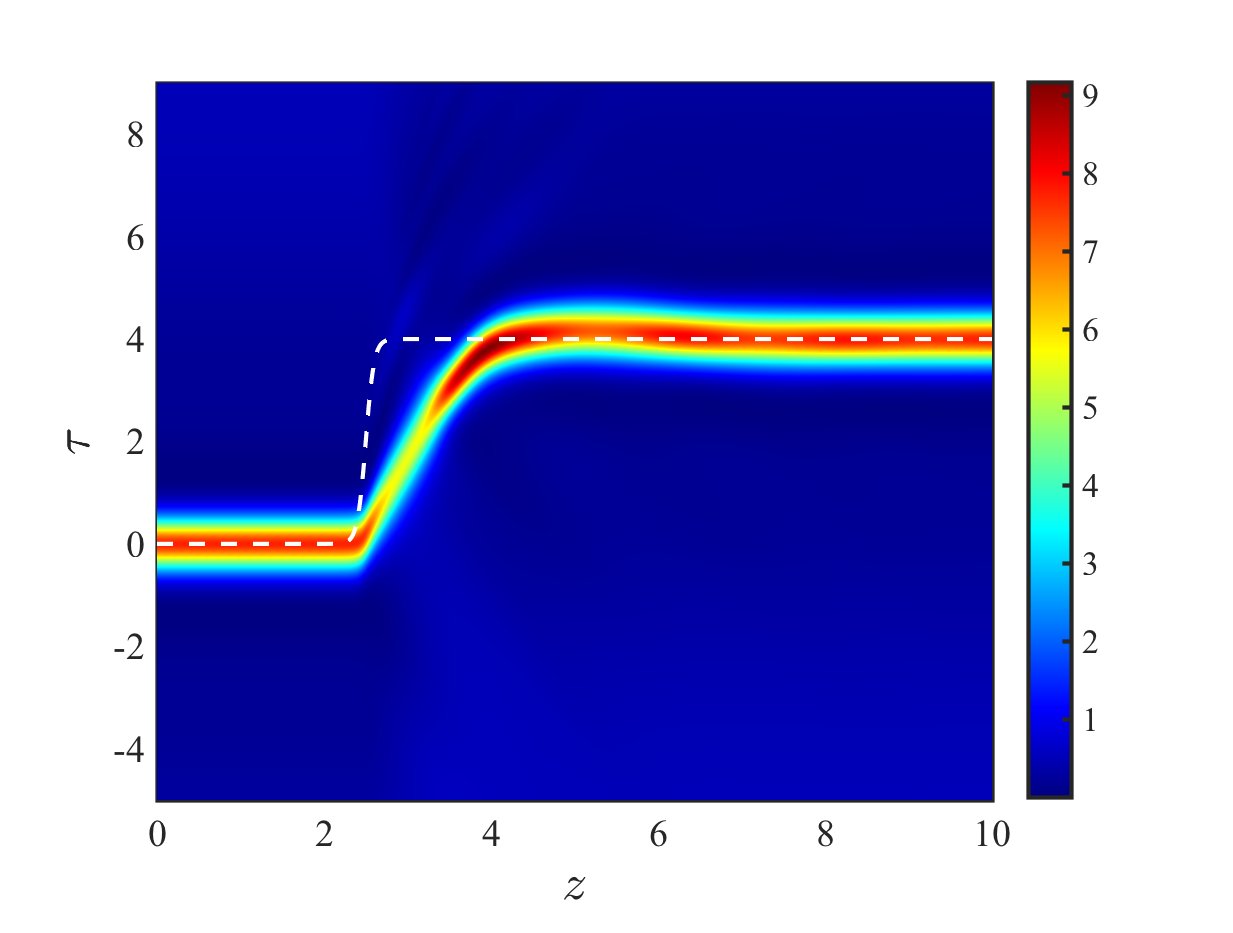
\includegraphics[width=\linewidth]{fatDensity1.eps} 
\caption{}
\end{subfigure}
\hspace*{-0.5cm}
\begin{subfigure}{0.5\textwidth}
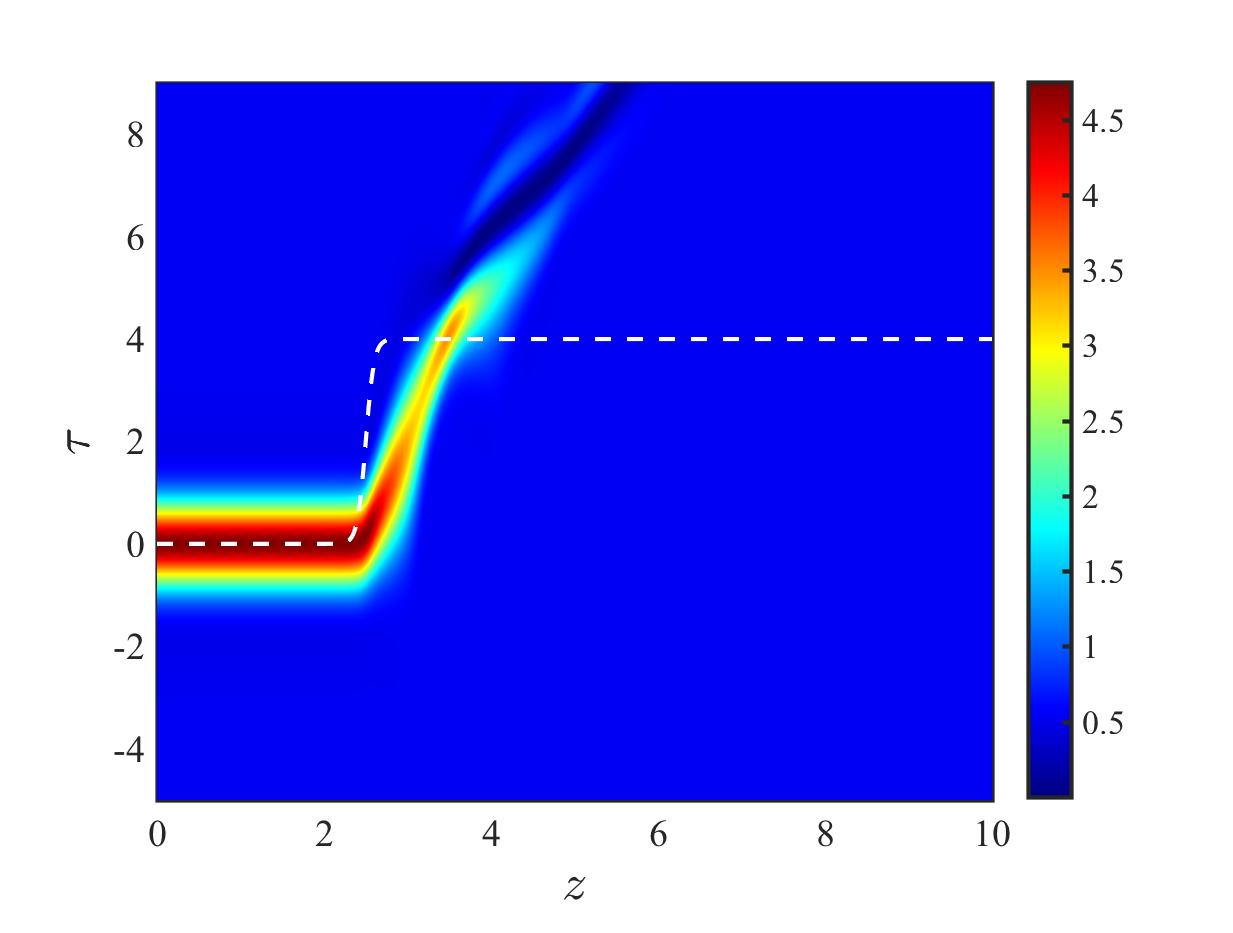
\includegraphics[width=\linewidth]{fatNCVADensity1.eps} 
\caption{}
\end{subfigure} }
\centerline{
%\hspace{1cm}
\begin{subfigure}{\textwidth}
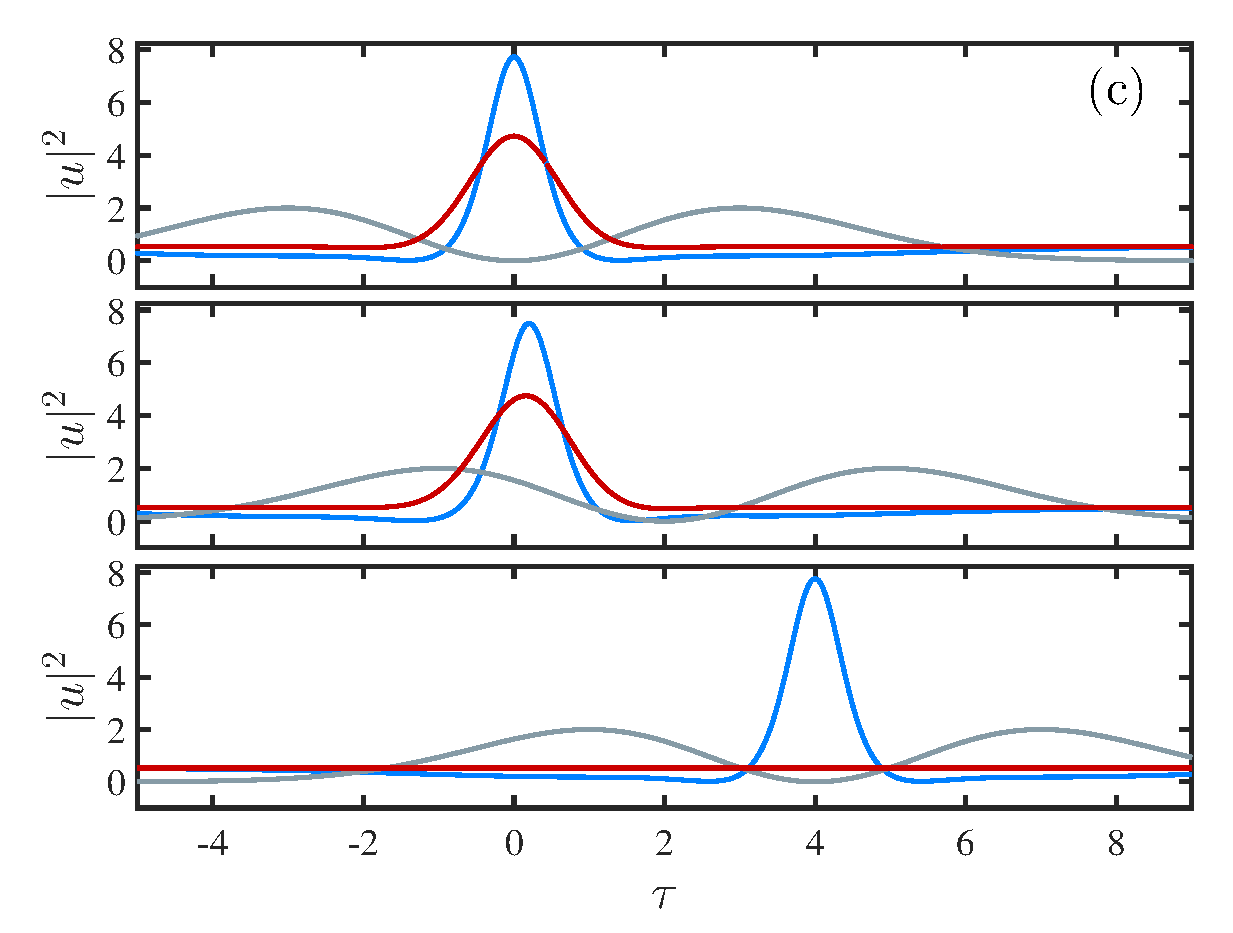
\includegraphics[width=\linewidth]{fatTimeSeries1.eps} 
\caption{}
\end{subfigure}}
  \rule{35em}{0.5pt}
\caption[Dynamic Evolution of Wide Tweezer with Tweezed CS]{Dynamic evolution as in Fig.~\ref{fig:Skinny1} but for $\tau_f = 4$ and $\beta = 10$.  Same layout as in Fig.~\ref{fig:Skinny1}.  In this sample, the NCVA solution is a no-CS, while the LL model is a tweezed-CS. 
}
\label{fig:Fat1}
\end{figure}

\begin{figure}[htb!]
\centering
\centerline{
\hspace{1cm}
\begin{subfigure}{0.5\textwidth}
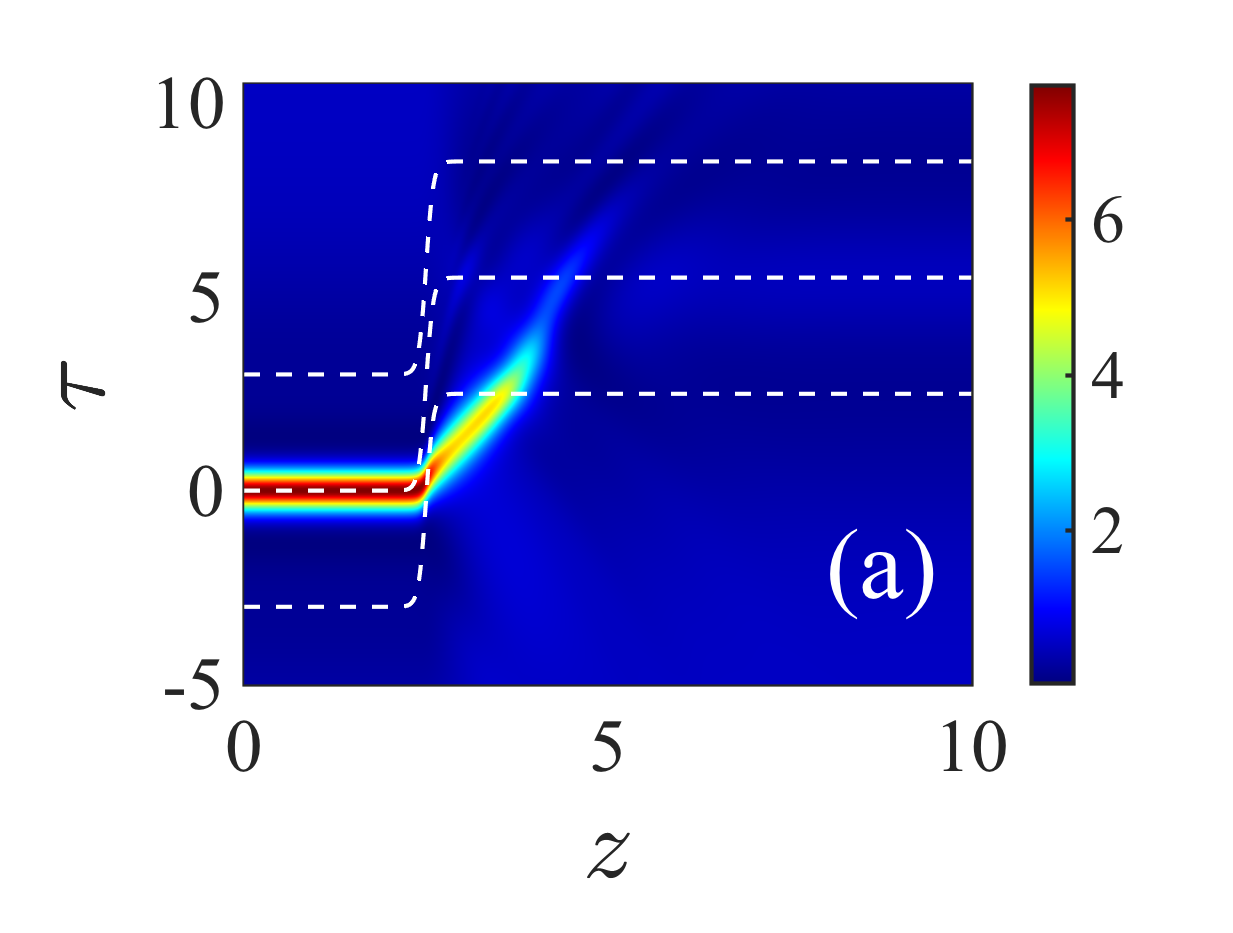
\includegraphics[width=\linewidth]{fatDensity2.eps} 
\caption{}
\end{subfigure}
\hspace{-1cm}
\begin{subfigure}{0.5\textwidth}
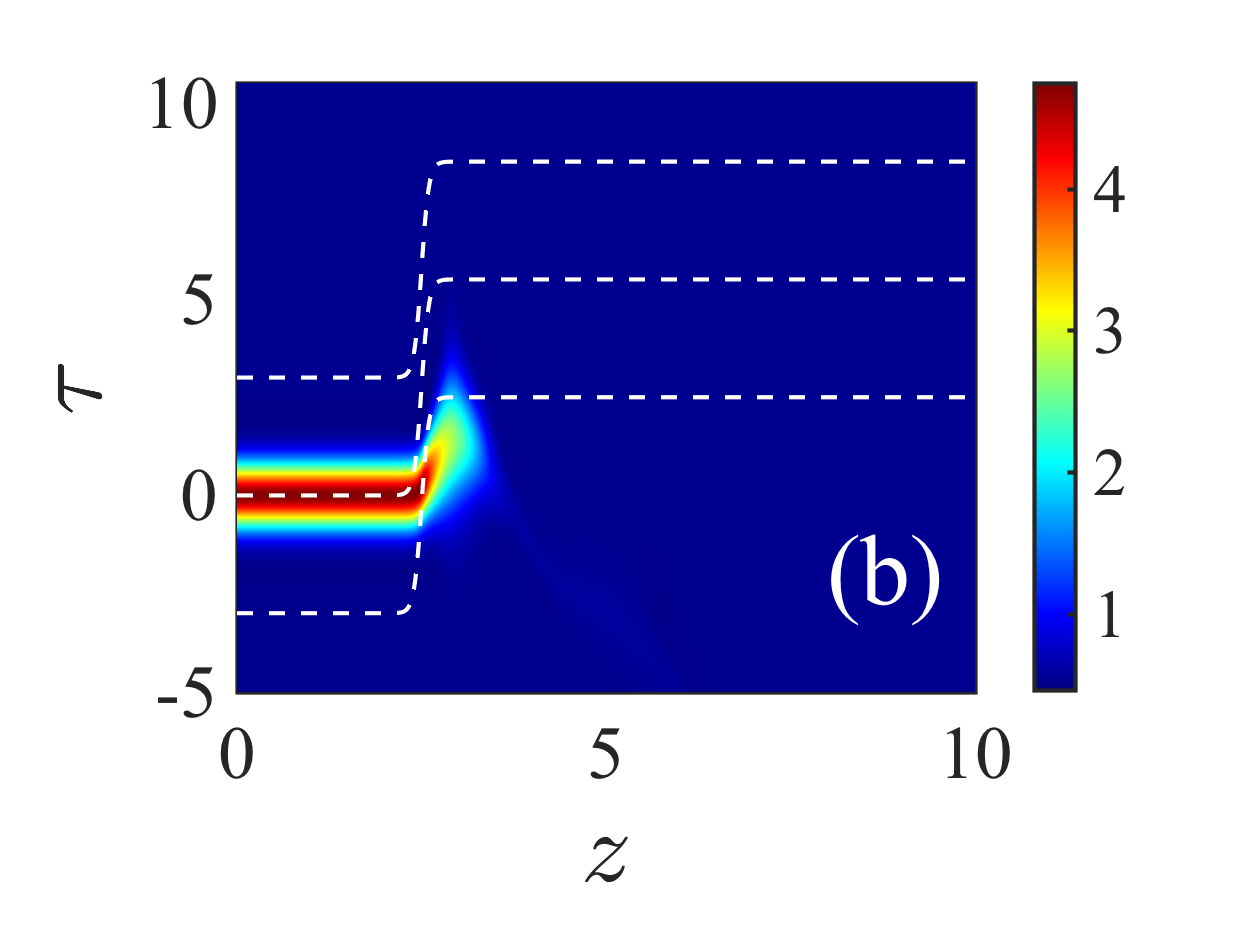
\includegraphics[width=\linewidth]{fatNCVADensity2.eps} %{fatNCVADensity2.eps} 
\caption{}
\end{subfigure} }
\centerline{
\hspace{1cm}
\begin{subfigure}{\textwidth}
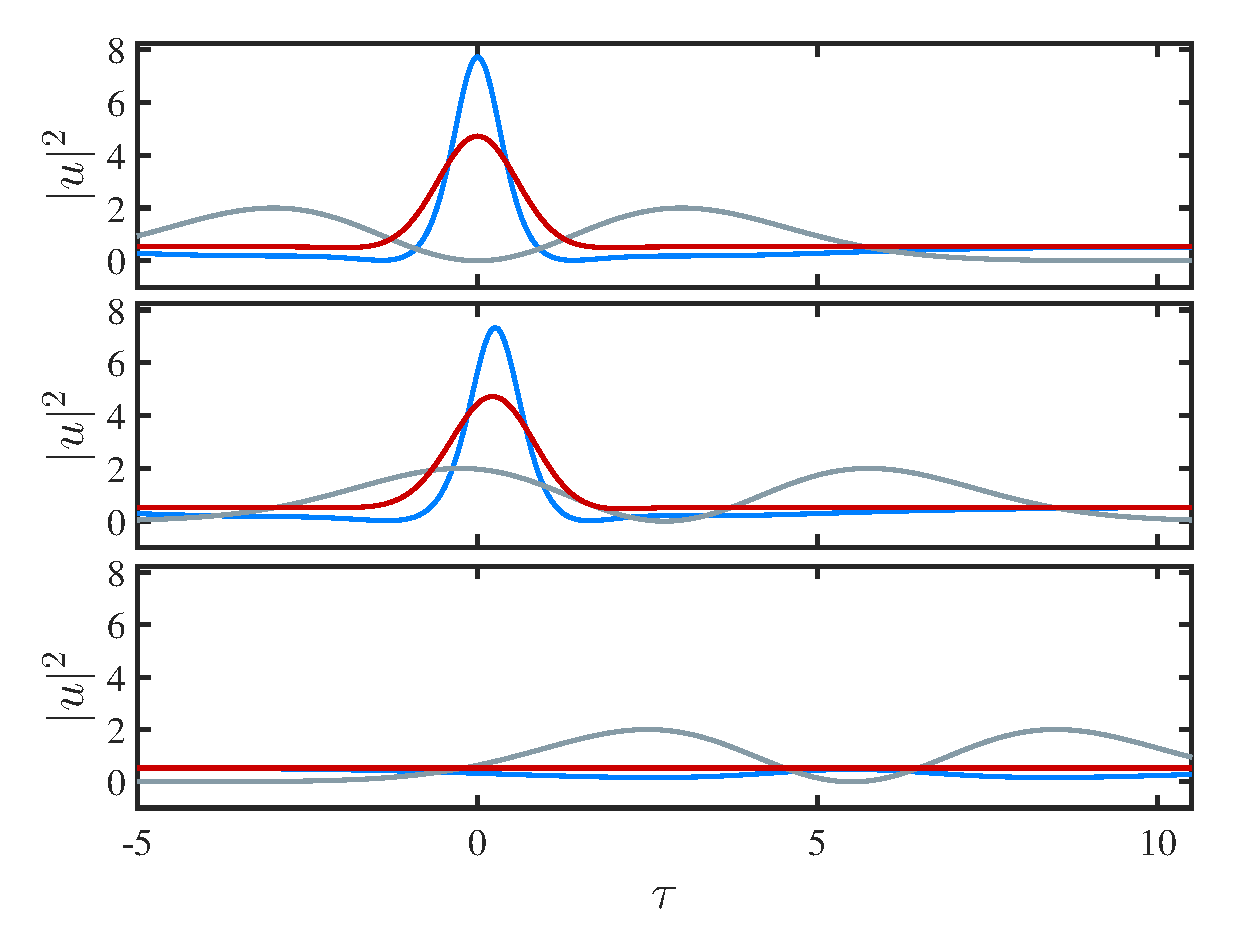
\includegraphics[width=0.9\linewidth]{fatTimeSeries2.eps} 
\caption{}
\end{subfigure}}
  \rule{35em}{0.5pt}
\caption[Dynamic Evolution of Wide Tweezer with no-CS]{Dynamic evolution as in Fig.~\ref{fig:Skinny1} but for $\tau_f = 5.5$ and $\beta = 10$.  Same layout as in Fig.~\ref{fig:Skinny1}.  In this sample, the NCVA and the full LL model is a no-CS.  }
\label{fig:Fat2}
\end{figure}

\begin{figure}[htb!]
\centering
\centerline{
\hspace{1cm}
\begin{subfigure}{0.5\textwidth}
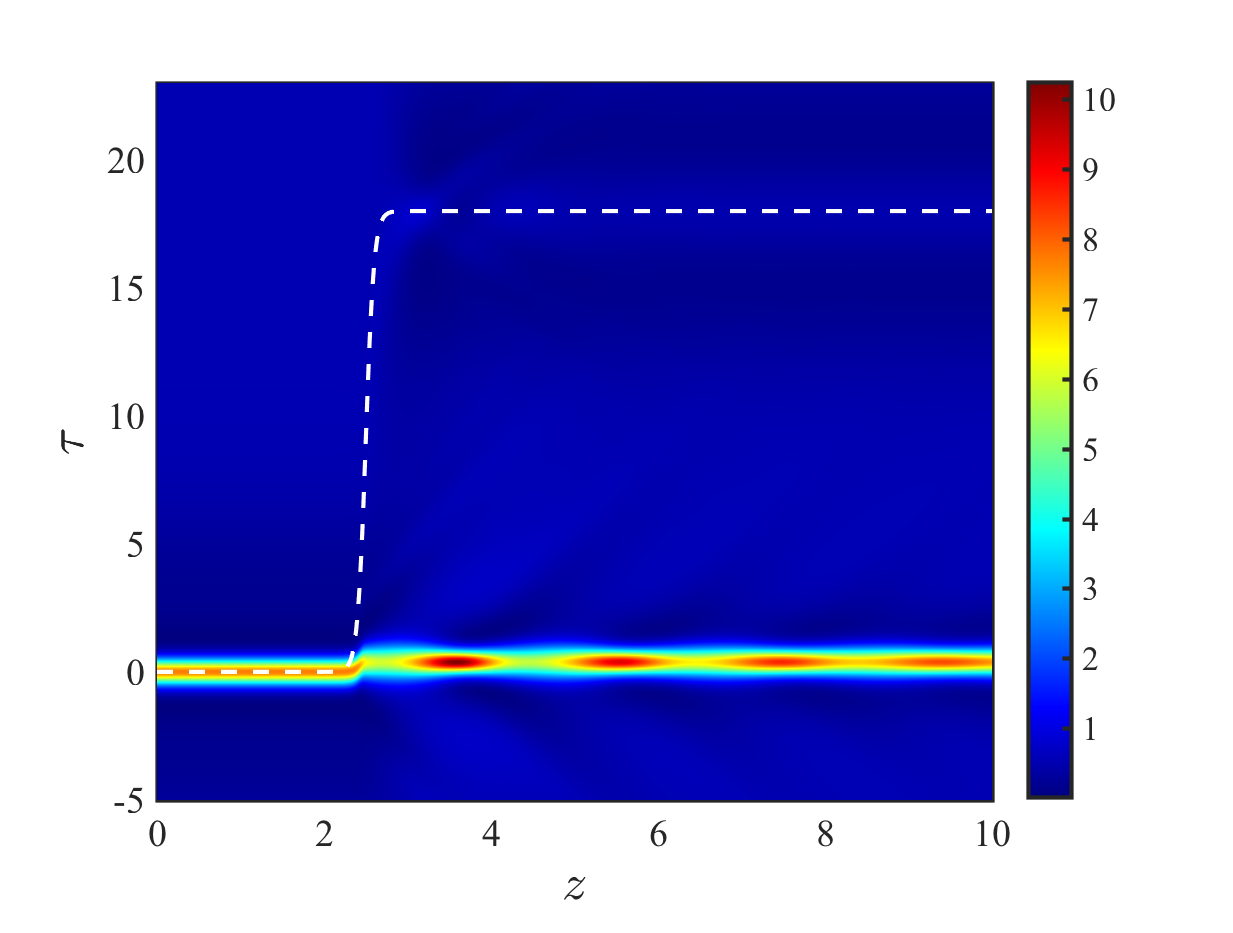
\includegraphics[width=\linewidth]{fatDensity3.eps} 
\caption{}
\end{subfigure}
\hspace{-1cm}
\begin{subfigure}{0.5\textwidth}
\includegraphics[width=\linewidth]{fatNCVADensity3.eps} %{fatNCVADensity3.eps} 
\caption{}
\end{subfigure} }
\centerline{
\hspace{1cm}
\begin{subfigure}{\textwidth}
\includegraphics[width=0.9\linewidth]{fatTimeSeries3.eps} 
\caption{}
\end{subfigure}}  \rule{35em}{0.5pt}
\caption[Dynamic Evolution of Wide Tweezer with Non-Tweezed CS]{Dynamic evolution as in Fig.~\ref{fig:Skinny1} but for $\tau_f = 18$ and $\beta = 10$.  Same layout as in Fig.~\ref{fig:Skinny1}.  In this sample, the NCVA solution is a no-CS.  The non-tweezed CS of the LL model is stationary outside the wide tweezer, which leaves the CS behind as the phase modulation is moved.
}
\label{fig:Fat3}
\end{figure}

\begin{figure}[htb!]
\centering
\centerline{
\hspace{1cm}
\begin{subfigure}{0.5\textwidth}
\includegraphics[width=\linewidth]{fatDensity5.eps} 
\caption{}
\end{subfigure}
\hspace{-1cm}
\begin{subfigure}{0.5\textwidth}
\includegraphics[width=\linewidth]{fatNCVADensity5.eps} 
\caption{}
\end{subfigure} }
\centerline{
\hspace{1cm}
\begin{subfigure}{\textwidth}
\includegraphics[width=0.9\linewidth]{fatTimeSeries5.eps} 
\caption{}
\end{subfigure}}
  \rule{35em}{0.5pt}
\caption[Dynamic Evolution of Wide Tweezer with Artificial Tweezing]{Dynamic evolution as in Fig.~\ref{fig:Skinny1} but for $\tau_f = 9$ and $\beta = 10$.  Same layout as in Fig.~\ref{fig:Skinny1}.  In this example, the NCVA is a no-CS.  The LL model has an ``artificially'' tweezed CS defined by the complete loss of the CS from the trap, but rather than a stationary CS left outside the trap (as is the case in non-tweezed CS), the CS is imparted with enough energy to continue moving in the direction of the tweezer.  By the final time $z_f$ the CS catches up with the tweezer and LL solutions are both no-CS. 
}
\label{fig:Fat4}
\end{figure}

As a sample of the dynamic properties of tweezability, Fig.~\ref{fig:Fat1} depicts a tweezed CS in the LL model and no-CS in the NCVA and Fig.~\ref{fig:Fat2} a no-CS for both the full LL model and the NCVA.  For the third sample, Fig.~\ref{fig:Fat3} the tweezer leaves the CS outside the effective potential in the full LL model while in the NCVA the solution is dissipative.  In contrast, Fig.~\ref{fig:Fat4} depicts the existence of artificial tweezing in the full LL model and a no-CS in the NCVA.  As Figs.~\ref{fig:Fat1}(a) and (b) show the initial state [see solid (blue) line LL model solution and solid (red) line NCVA solution in Fig.~\ref{fig:Fat1}(c) top panel] is manipulated by the wide tweezer towards $\tau_f$ at speed $\beta$ [see solid (blue) line LL model solution and solid (red) line NCVA solution in Fig.~\ref{fig:Fat1}(c) bottom panel], which we refer to as a tweezed CS in the LL model and no-CS in the NCVA.  Figures~\ref{fig:Fat2}(a) and (b) show the initial state [see solid (blue) line LL model solution and solid (red) line NCVA solution in Fig.~\ref{fig:Fat2}(c) top panel] is dragged by the wide tweezer for a short time before being lost in the LL model whereas the NCVA is only a no-CS solution [see solid (blue) line LL model solution  and solid (red) line NCVA solution in Fig.~\ref{fig:Fat2}(c) bottom panel].  As Figs.~\ref{fig:Fat3}(a) and (b) show the initial state [see solid (blue) line LL model solution and solid (red) line NCVA solution in Fig.~\ref{fig:Fat3}(c) top panel] is left behind as the wide tweezer is displaced for the LL model and is completely lost in the case of the NCVA  [see solid (blue) line LL model solution  and solid (red) line NCVA solution in Fig.~\ref{fig:Fat3}(c) bottom panel].  For the artificial tweezing dynamic properties, Figs.~\ref{fig:Fat4}(a) and (b) show the initial state [see solid (blue) line LL model solution and solid (red) line NCVA solution in Fig.~\ref{fig:Fat4}(c) top panel] is manipulated by the wide tweezer towards $\tau_f$ at speed $\beta$ [see solid (blue) line LL model solution and solid (red) line NCVA solution in Fig.~\ref{fig:Fat4}(c) bottom panel], and as the CS is dragged the solution is initial lost in the LL model, but catches back up and is re-trapped by the tweezer at $z_f$. 

Along with the three cases described here, Appendix~\ref{AppendixC} displays other thresholds given by the density of the power ratios for extra tweezers with $h_\phi =2$ and $\sigma_\phi$ = 0.5, 1, and 2, respectively.

\JMR{\subsection{Demonstration of Temporal Tweezing}
 \label{section:FinalExample}
Next, we demonstrate the temporal tweezing of a trapped CS given our knowledge of parameter space $\tau_f$ and $\beta$.  Figure~\ref{fig:Final} is the dynamic properties of tweezability for both the full LL model and the NCVA with a natural width tweezer.  In Fig.~\ref{fig:Final}, instead of a single value of $\tau_f$ and $\beta$ we change the parameters at set increments of slow time $z$.  For $z\le5$, $\tau_f$=2 and $\beta$ = 10, then for $5 < z\le10$, $\tau_f$=0 and $\beta$ = 10, then for $10 < z\le15$, $\tau_f$=3 and $\beta$ = 0.5, then for $15 < z\le20$, $\tau_f$=1 and $\beta$ = 20, then for $20 < z\le25$, $\tau_f$=-2 and $\beta$ = 0.5.  The LL model [Fig.~\ref{fig:Final}(a)] and NCVA [Fig.~\ref{fig:Final}(b)] dynamics are in agreement with the expected tweezed-CS and also with each other.  In the NCVA, Fig.~\ref{fig:Final}(b) has an additional black line depicting the ansatz parameter $\xi$ which follows the center position of the tweezer $\tau_0$.  The example is designed to illustrate how the phase-modulation can move the trapped CS with different speeds at will.  }
 
%%%%%%%%%% Fig  %%%%%%%%%%%%%%%%%%%%%%%%%%%%%%%%%%%%%%
\begin{figure}[htb!]
\centering
\includegraphics[width=0.7\textwidth]{regularDensityFinal.eps} \\
\centerline{\includegraphics[width=0.7\textwidth]{regularNCVADensityFinal.eps} }
  \rule{35em}{0.5pt}
  \caption[Temporal Tweezing of a CS]{Dynamic evolution as in Fig.~\ref{fig:Skinny1} but for variable $\tau_f$ and $\beta$.  Same layout as in Fig.~\ref{fig:Skinny1}(a) and (b).  In this sample, we illustrate how a CS can be discretely manipulated given various parameters of $\tau_f$ and $\beta$.  The LL model (a) and NCVA (b) solution are continusously tweezed as the tweezer moves at various speeds.  The dashed white lines are the center of $\tau_0(z)$ and $\pm \sigma_\phi$.  In panel (b) the black line is the NCVA variational parameter $\xi$.
}
\label{fig:Final}
\end{figure}
%%%%%%%%%% Fig  %%%%%%%%%%%%%%%%%%%%%%%%%%%%%%%%%%%%%%

\setstretch{1.3}
\section[Summary]{Summary} \label{section:TweezeSummary}
\setstretch{2}

%The chapter served to define regions of tweezability for CSs in the presence of a Gaussian phase-modulation used as a tweezer.  We identified three states: a tweezed CS, a no-CS, and a non-tweezed CS.  We used narrow, natural, and wide width tweezers to study regions of existence for CS states.  In this chapter we also applied the NCVA to the LL model describing tweezed temporal cavity solitons.  The NCVA is capable of predicting a threshold of phase-modulation parameters between tweezed CS and no-CS state.     
%
In summary, we studied an LL equation modified to include a controllable temporal phase modulation introduced through $\phi(\tau, z)$ to describe temporal tweezing of CSs.  Our motivation was to understand when the parameters of the phase modulation were adequate to successfully tweeze the CS and when they failed.  We found thresholds for tweezing a CS dependent on the total displacement and the speed of the tweezer.  In our analysis, we also found that the shape of the tweezer impacts these regions and can have a dramatic effect on the dynamics of the CS.  The narrow tweezer is a bad candidate for tweezing, but the natural and wide width tweezers can give good control and manipulation of a CS.  In the full LL model there are three fundamental states: a tweezed CS, a non-tweezed CS and a no-CS. By contrast, the NCVA only describes two states: a tweezed CS and a no-CS.  Instead of full analysis of the LL model, we can use the NCVA to determine a lower bound on the threshold for phase modulation parameters where there exists temporal tweezing of a CS.  

A very interesting extension of the temporal tweezing study is to analyze the linearization spectrum of the system and identify the stability/instability transitions between the three states we identified.  In this same vein, the identification of the spectrum can be used with the center manifold approach capable of capturing bifurcations induced by changing the speed of the tweezer.  From our study of the LL equation and NCVA, we have developed a process to identify regions of tweezability which can aid experimental design and reliability of temporal tweezing used for information processing.
 





